% ----------------------------------------------------
% Introduction
% ----------------------------------------------------
\documentclass[class=report,11pt,crop=false]{standalone}
% Page geometry
\usepackage[a4paper,margin=20mm,top=25mm,bottom=25mm]{geometry}

% Font choice
\usepackage{lmodern}

% Wrap text around image
\usepackage{wrapfig}

% Checkmarks
\usepackage{tikz}

% For algorithms
\usepackage[]{algorithm}
% Pseudocode packages
\usepackage{algpseudocode}

% Table color
% \usepackage{colortbl}

% Multiple rows
\usepackage{multirow}

% Lorem ipsum
\usepackage{lipsum}

% Use IEEE bibliography style
\bibliographystyle{IEEEtran}

% Line spacing
\usepackage{setspace}
\setstretch{1.20}

% Ensure UTF8 encoding
\usepackage[utf8]{inputenc}

% Language standard (not too important)
\usepackage[english]{babel}

% Skip a line in between paragraphs
\usepackage{parskip}

% For the creation of dummy text
\usepackage{blindtext}

% Math
\usepackage{amsmath}

% Lists
\usepackage{enumitem}

% Header & Footer stuff
\usepackage{fancyhdr}
\pagestyle{fancy}
\fancyhead{}
\fancyhead[R]{\nouppercase{\rightmark}}
\fancyfoot{}
\fancyfoot[C]{\thepage}
\renewcommand{\headrulewidth}{0.0pt}
\renewcommand{\footrulewidth}{0.0pt}
\setlength{\headheight}{13.6pt}

% Epigraphs
\usepackage{epigraph}
\setlength\epigraphrule{0pt}
\setlength{\epigraphwidth}{0.65\textwidth}

% Colour
\usepackage{color}
%\usepackage[usenames,dvipsnames]{xcolor}

% Hyperlinks & References
\usepackage{hyperref}
\definecolor{linkColour}{RGB}{77,71,179}
\hypersetup{
    colorlinks=true,
    linkcolor=linkColour,
    filecolor=linkColour,
    urlcolor=linkColour,
    citecolor=linkColour,
}
\urlstyle{same}

% Automatically correct front-side quotes
\usepackage[autostyle=false, style=ukenglish]{csquotes}
\MakeOuterQuote{"}

% Graphics
\usepackage{graphicx}
\graphicspath{{Images/}{../Images/}}
\usepackage{makecell}
\usepackage{transparent}

% SI units
\usepackage{siunitx}

% Microtype goodness
\usepackage{microtype}

% Listings
\usepackage[T1]{fontenc}
\usepackage{listings}
\usepackage[scaled=0.8]{DejaVuSansMono}

% Custom colours for listings
\definecolor{backgroundColour}{RGB}{250,250,250}
\definecolor{commentColour}{RGB}{73, 175, 102}
\definecolor{identifierColour}{RGB}{196, 19, 66}
\definecolor{stringColour}{RGB}{252, 156, 30}
\definecolor{keywordColour}{RGB}{50, 38, 224}
\definecolor{lineNumbersColour}{RGB}{127,127,127}
\lstset{
  language=Matlab,
  captionpos=b,
  aboveskip=15pt,belowskip=10pt,
  backgroundcolor=\color{backgroundColour},
  basicstyle=\ttfamily,%\footnotesize,        % the size of the fonts that are used for the code
  breakatwhitespace=false,         % sets if automatic breaks should only happen at whitespace
  breaklines=true,                 % sets automatic line breaking
  postbreak=\mbox{\textcolor{red}{$\hookrightarrow$}\space},
  commentstyle=\color{commentColour},    % comment style
  identifierstyle=\color{identifierColour},
  stringstyle=\color{stringColour},
   keywordstyle=\color{keywordColour},       % keyword style
  %escapeinside={\%*}{*)},          % if you want to add LaTeX within your code
  extendedchars=true,              % lets you use non-ASCII characters; for 8-bits encodings only, does not work with UTF-8
  frame=single,	                   % adds a frame around the code
  keepspaces=true,                 % keeps spaces in text, useful for keeping indentation of code (possibly needs columns=flexible)
  morekeywords={*,...},            % if you want to add more keywords to the set
  numbers=left,                    % where to put the line-numbers; possible values are (none, left, right)
  numbersep=5pt,                   % how far the line-numbers are from the code
  numberstyle=\tiny\color{lineNumbersColour}, % the style that is used for the line-numbers
  rulecolor=\color{black},         % if not set, the frame-color may be changed on line-breaks within not-black text (e.g. comments (green here))
  showspaces=false,                % show spaces everywhere adding particular underscores; it overrides 'showstringspaces'
  showstringspaces=false,          % underline spaces within strings only
  showtabs=false,                  % show tabs within strings adding particular underscores
  stepnumber=1,                    % the step between two line-numbers. If it's 1, each line will be numbered
  tabsize=2,	                   % sets default tabsize to 2 spaces
  %title=\lstname                   % show the filename of files included with \lstinputlisting; also try caption instead of title
}

% Caption stuff
\usepackage[hypcap=true, justification=centering]{caption}
\usepackage{subcaption}

% Glossary package
% \usepackage[acronym]{glossaries}
\usepackage{glossaries-extra}
\setabbreviationstyle[acronym]{long-short}

% For Proofs & Theorems
\usepackage{amsthm}

% Maths symbols
\usepackage{amssymb}
\usepackage{mathrsfs}
\usepackage{mathtools}

% For algorithms
%\usepackage[]{algorithm2e}

% Spacing stuff
\setlength{\abovecaptionskip}{5pt plus 3pt minus 2pt}
\setlength{\belowcaptionskip}{5pt plus 3pt minus 2pt}
\setlength{\textfloatsep}{10pt plus 3pt minus 2pt}
\setlength{\intextsep}{15pt plus 3pt minus 2pt}

% For aligning footnotes at bottom of page, instead of hugging text
\usepackage[bottom]{footmisc}

% Add LoF, Bib, etc. to ToC
\usepackage[nottoc]{tocbibind}

% SI
\usepackage{siunitx}

% For removing some whitespace in Chapter headings etc
\usepackage{etoolbox}
\makeatletter
\patchcmd{\@makechapterhead}{\vspace*{50\p@}}{\vspace*{-10pt}}{}{}%
\patchcmd{\@makeschapterhead}{\vspace*{50\p@}}{\vspace*{-10pt}}{}{}%
\makeatother
\makenoidxglossaries

\newacronym{radar}{RADAR}{Radio Detection and Ranging}
\begin{document}
	% ----------------------------------------------------
	\chapter{Methodology \label{ch:meth}}
	%\epigraph{Philosophers have hitherto only interpreted the world in various ways; the point is to change it.}%
	%    {\emph{---Karl Marx}}
	%\vspace{0.5cm}
	% ----------------------------------------------------
	
	%\lipsum[1]
	\section{Methodology Outline}
	
	This chapter details the design process and approach employed in achieving the aim of the project which is to  digitize and modernize the HP141T display by replacing the \acrshort{crt} monitor with a \acrshort{lcd} touchscreen display that offers different functions and modes of operation. Design decision are also documented here, showing the considerations that were made based on the operation and outputs of the HP141T spectrum analyzer and ensuring that the newly integrated display is compatible with the device's hardware. For example, the design required selection of the digital hardware for processing the analog voltage signals from the \acrshort{sa}. The selection of the digital processor made from single-board computers such as the Raspberry Pi 4 Model B, microcontrollers like the STM32F4 boards, \acrshort{fpga} such as the Artix-7 from Xilinix, or a heterogeneous digital processor which consists of a combination of these options. 
	
	Other considerations were made regarding the electronic circuits for converting the auxiliary output voltages from the HP141T to the appropriate voltage level for the operation of \acrshort{adc}. This chapter describes how together, the \acrshort{adc} and digital processor form a crucial part of the system. Additionally, the chapter details the software development kit (\acrshort{sdk}) and associated coding language that was used. The selection of the development framework depended on the choice of processor and digital processing algorithms that were required to fulfil the project requirements. For example, assuming that a \acrshort{fpga} is the chosen digital processor, the  \acrshort{sdk} would include tools such as the AMD Vivado and electronic design automation (\acrshort{eda}) software and the choice of coding language between Verilog, VHDL, and SystemVerilog would depend on how comfortable the developer is in representing digital processing algorithms, such the \acrshort{dft}, using the chosen language. 
	
	Overall, this chapter documents an overview of the design methodology and different phases in the design process. The design process followed a variation of V-Model in which a series of iterative phases was implemented with a process checking mechanism. The chapter begins by highlighting the design stages and modularization of the system. Thereafter, the chapter includes an assessment of the project requirements detailed in introductory section. Finally, the chapter describes the use of findings from the review of requirements in informing the design decisions and specifications.  
	
	\section{Phases in the Design Process}
	
	The design process was decomposed into four iterative stages as illustrated in Figure \ref{fig:design-stages-diagram} below. The first stage documented the digitization requirements and listed examples of modern \acrshort{sa}s in order to define the requirements for modernization. As shown in the methodology overview diagram, the first stage also included thorough investigation into methods that have been implemented in literature for upgrading the functions and performance of \acrshort{sa}s. A theoretical framework for relevant information about signal processing was also formulated based on the literature to ensure that the display modes and functions were consistent with the mathematically derived expected outputs in the system. 
	
	\begin{figure}[!ht]
		\centering
		\label{fig:design-stages-diagram}
		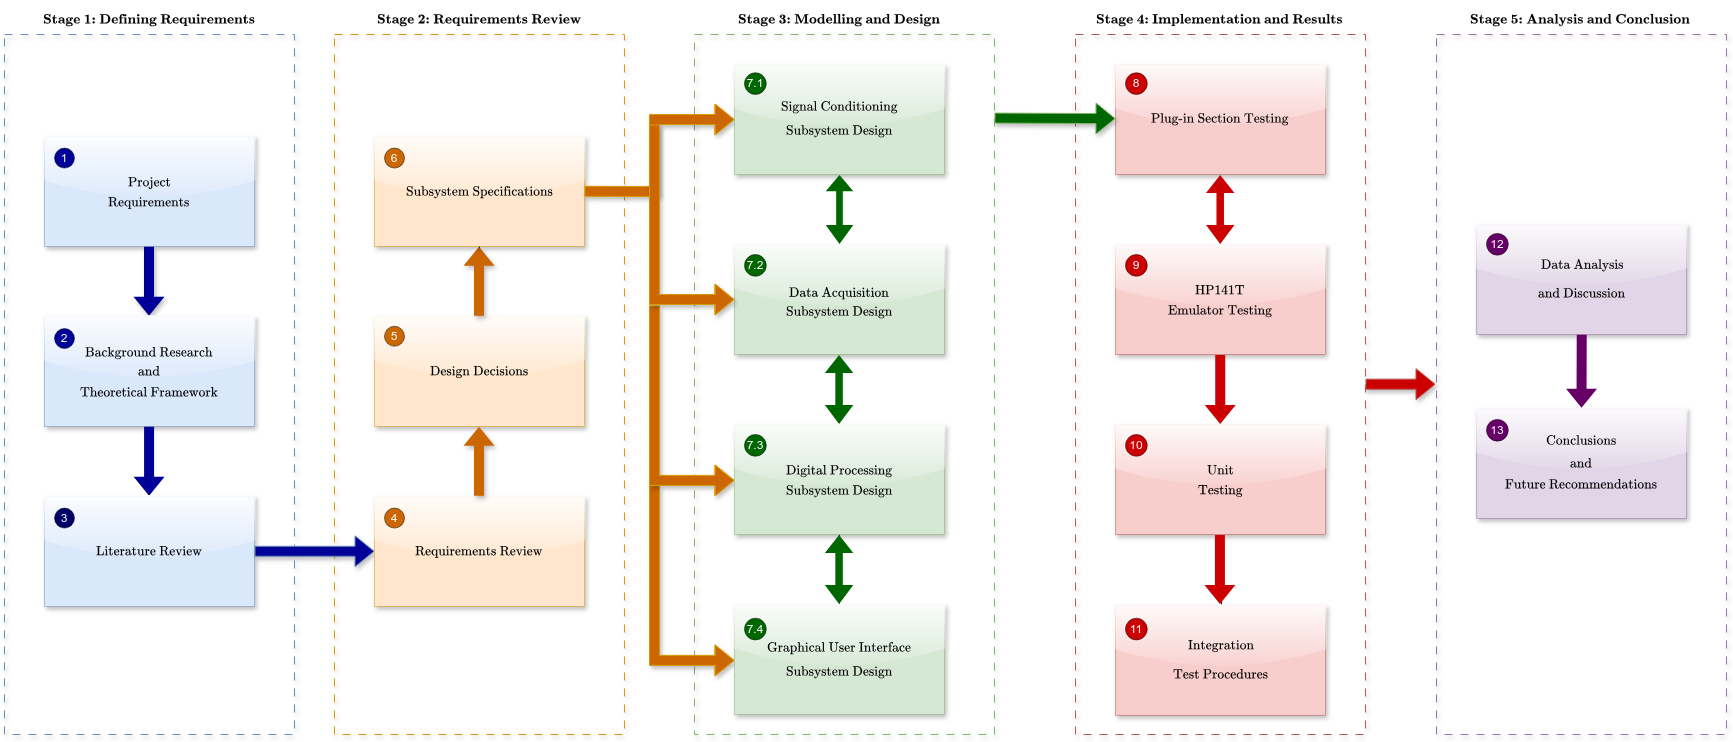
\includegraphics[width=1.0\linewidth]{Figures/Methodology/design-stages-diagram.png}
		\caption{Methodology overview showing different stages in the iterative design process that was applied as a variation of the V-Model.}
	\end{figure}
	
	The second stage in the design process involved a review of the user requirements specifications detailed in chapter \ref{ch:intro}. The aim of this step in the methodology was to clarify the desired functions of the upgraded spectrum analyzer and to inform the design decisions with respect to the digital hardware and software development for digital signal processing. Additionally, the requirements review was employed in modularizing the design into four subsystems including, the Analog-to-Digital Conversion, Digital Processing, Screen and User Interface subsystems. 
		
	Stage 3 of the design process dealt with the design specifications of each of these subsystems by further decomposing each module into smaller hardware and software components. Each function is tested against a requirement in Stage 4 where each design specification was verified and the operation of the integrated system was tested to ensure that the interfaces between the subsystems was configured correctly. 
	
	In general, implementation of the design process adhered to the following design steps detailed in the project brief and are associated with the user requirement specifications:
	
	\begin{enumerate}
		\item 
		Surveying the HP141T display and other outputs.
		\item 
		Surveying single-board computers and touchscreen options.
		\item 
		Phase One: establish a basic XYZ replica or HP141T emulator.
		\item 
		Phase Two: implement averaging and peak hold options.
		\item 
		Phase Three: annotate display axes.
		\item 
		Phase Four: determine the appropriate instrument settings. 
		\item 
		Phase Five: design new annotations for display taking instrument or operator manual inputs into account.
		\item 
		Phase Six: include more tutorial and operational instructions using.
	\end{enumerate}
	
	In finalizing the design process of the upgraded \acrshort{sa}, results from acceptance tests were assimilated and a conclusion was drawn. Then, based on the outcomes of the project, future recommendations were made for future iterations of the upgrade \acrshort{sa} system. Overall, the stages of the methodology included:
	
	\begin{itemize}
		\item 
		Stage 1: Defining Requirements
		\item 
		Stage 2: Requirements Review and System Overview
		\item 
		Stage 3: Modelling and Design
		\item 
		Stage 4: Implementation and Results
		\item 
		Stage 5: Analysis and Conclusion 
	\end{itemize}

	The first four stages of the design process were performed iteratively as a variation of the V-Model in which risk analysis was performed at each step, similar to the Spiral Model for design processes. Each iteration aimed at producing a new version of the upgraded HP141T display and a single conclusion was made when a satisfactory prototype was established.

	\section{Requirements Review}
	
	This section aims to clarify the scope of the project and produce a technical formalization of the user requirements specifications. The section begins by giving context to the term modernization by investigating the properties of modern \acrshort{sa}s. Then, the section breaks down the user requirements into categories relating data acquisition, processing and display. Finally, the section concludes with a review of the requirement for developing a HP141T emulator. 
		
	\subsection{Comparing the HP141T System to Modern Spectrum Analyzers}
	
	The first user requirement deals with the modernization of the HP141T system. The aim of this section is to review this requirement and to give clarification on the context of the use of "modernization" in this project. To achieve this objective, the section begins with a description of the HP141T system and the functions that differ from "modern" spectrum analyzers, such as the range of hand-held \acrshort{sa}s by FieldFox, and the N9000B CXA \acrshort{sa} manufactured by Keysight\textregistered. The section concludes with a summary table comparing the features of the HP141T system and modern spectrum analyzers. 
	
	The HP141T system is equipped with three plug-ins, namely the 8555A \acrshort{rf} section which operates in the microwave region of the electromagnetic spectrum, the 8552B \acrshort{if} section and the Model 141T display which includes the \acrshort{crt} monitor. The three plug-ins operate in unison to electronically scan signals in the time-domain and provide a visual representation of the input signal's amplitude in the frequency domain on the \acrshort{crt} monitor \cite{HP8555A}. Amplitude can be represented on a logarithmic ($\si{\decibel\meter}$) or linear scale ($\si{\milli\volt}$). 
	
	The 8555A and 8552B plug-ins apply principles of heterodyning spectroscopy, allows high frequency input signals with frequencies in the K-band of the microwave portion of the electromagnetic spectrum (i.e. $\SI{18}{\mega\hertz}$) \cite{harris2003}. As noted from literature in the previous chapter, spectrum analyzers which rely on the \acrshort{fft} by sampling the continuous input signal and performing the Fourier transform on $N$ total samples typically deal with signals that have lower frequencies. This is because \acrshort{sa}s that employ the super-heterodyne principle like the HP141T determine the spectrum directly by analysis in the frequency domain and not from the time-dependent characteristics of the input signal. This is achieved by using a super-heterodyne receiver comprised of a mixer and tunable local oscillator (\acrshort{lo}) which convert the input signal to an intermediate frequency as illustrated in figure \ref{fig:heterodyne-rauscher} \cite{rauscher2007}. 
	
	\begin{figure}[!ht]
		\centering
		\label{fig:heterodyne-rauscher}
		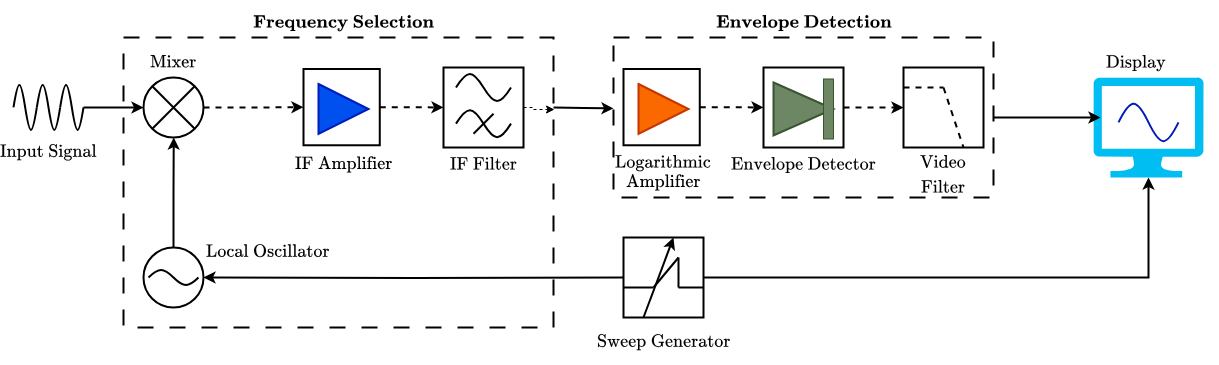
\includegraphics[width=1.0\linewidth]{Figures/Methodology/heterodyne-rauscher.png}
		\caption{Heterodyne Spectrum Analyzer Block Diagram.}
	\end{figure}
	
	As noted in the literature review, most modern \acrshort{sa}s are real-time spectrum analyzers \acrshort{rtsa} which are a special case of vector spectrum analyzers (\acrshort{vsa}) that use the super-heterodyne principle but digitize the input signal at the intermediate frequency, as shown in Figure \ref{fig:vector-analyzer-rover}, using a bandpass filter which can behave like a pre-select filter to limit distortions that arise from the mixer and shows the result in real-time. The advantage of digitizing the output of the \acrshort{if} section is that it enables large a input range of up to $\SI{50}{\mega\hertz}$ which can be analyzed in the time and frequency domain using digital signal processing techniques \cite{rovers2006}. Much like \acrshort{fft} analyzers, vector analyzers are limited by the minimum and maximum sampling rate at which the \acrshort{adc} can operate. Additionally, exceedingly high sampling rates can lead to aliasing which causes frequencies outside of the bandwidth to fold into the frequency band \cite{rovers2006}. 	

	\begin{figure}[!ht]
		\centering
		\label{fig:vector-analyzer-rover}
		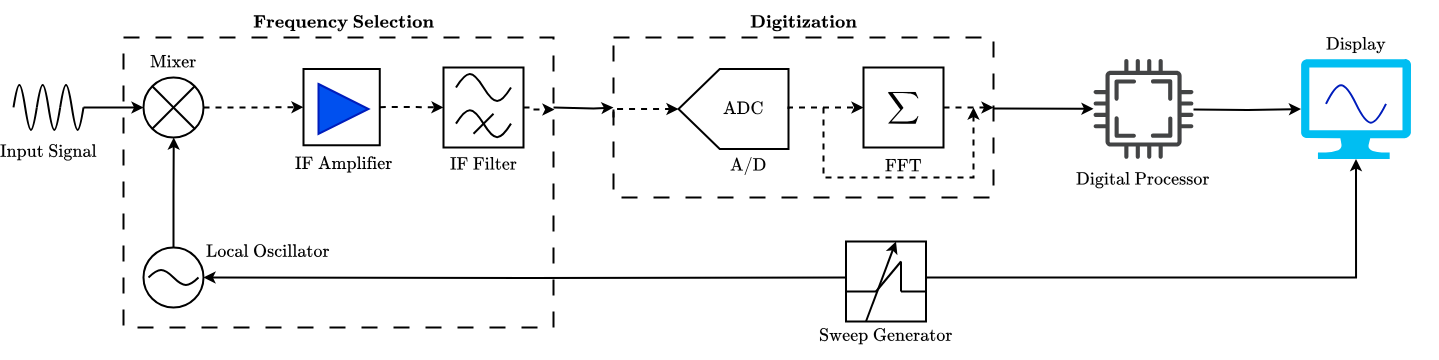
\includegraphics[width=1.0\linewidth]{Figures/Methodology/real-time-analyzer-rover.png}
		\caption{Vector analyzer block diagram showing digitization of the \acrshort{if} frequency.}
	\end{figure}

	Examples of modern real-time analyzers include:
	
	\begin{itemize}
		\item 
		Tektronix RSA2208A which can scan input signals with frequencies of up to $\SI{8}{\giga\hertz}$.
		\item 
		Rohde \& Schwarz FSP13 which operates within a $\SI{9}{\giga\hertz}$ to $\SI{30}{\giga\hertz}$ \acrshort{rbw}.
		\item
		Agilent E4445A which offer frequency analysis up to $\SI{13.2}{\giga\hertz}$.
		\item 
		FieldFox RTSA which covers $\SI{5}{\kilo\hertz}$ up to $\SI{50}{\giga\hertz}$.
	\end{itemize}

	In modern \acrshort{rtsa}s, \acrshort{if} analog output is transferred to the \acrshort{adc} through an anti-aliasing filter before being stored in memory \cite{tektronixRSA2208A}. This is in contrast to older heterodyne \acrshort{sa}s such as the HP141T which takes the \acrshort{if} output through a video filter is essentially an averaging low-pass filter which smooths the \acrshort{if} output and reduces the effects of internal noise before the signal is channelled to the display \cite{rauscher2007}. HP141T video filters may select $\SI{10}{\hertz}$, $\SI{100}{\hertz}$, $\SI{10}{\kilo\hertz}$ or OFF section of the low-pass filter for the detected video. 
	
	The output of the the HP141T video filter is transmitted to the vertical deflection of the \acrshort{crt} display \cite{HPsiganalyzers}. For the horizontal deflection of the electron beam in the \acrshort{crt} display, a sawtooth signal from the sweep generator governs the horizontal scaling of the output frequency as electrons impinge on the phosphorescent screen. Modern \acrshort{sa}s retrieve data from memory through high speed data lines to display information about the digital signal from the \acrshort{adc}. Digital display technologies include:
	
	\begin{itemize}
		\item 
		\acrshort{lcd} - most commonly used digital display which represents signal data with a sharp image and has low power consumption
		\item 
		\acrshort{oled} - typically used in high performance \acrshort{sa}s for displaying color coded spectrograms
		\item 
		\acrshort{tft} - offer good visual quality and response time for sharper imagery when analyzing high frequency signals.
	\end{itemize}

	Displays in modern \acrshort{sa} architectures offer more options for displaying frequency domain data. This is enabled by the processor, which is typically hosted on microcontroller board with high clock speed for performing digital signal processing algorithms. For example, \acrshort{rtsa}s display the spectrogram as a color coded function of the amplitude of the signal \cite{al2013}. In addition, digital displays generally consume less physical space compared to \acrshort{crt} displays with the same screen dimensions. This has allowed spectrum analyzers to become smaller as they entire system can fit into smaller packaging. For example, the FieldFox is an hand-held \acrshort{rtsa} which despite its size, offers improved performance over the HP141T.
	
	The comparison table in \ref{tab:comparing-old-to-modern} below summarizes the differences between the HP141T analyzer (equipped with the 8555A and 8552B plug-ins) and modern \acrshort{rtsa}s.
	
	 \begin{table}[ht!]
	 	\centering
	 	\begin{tabular}{|m{8em}|m{15em}|m{15em}|}
	 		\hline
	 		\cellcolor{cyan!25}\textbf{Feature}	& \cellcolor{cyan!25}\textbf{HP141T}	& \cellcolor{cyan!25}\textbf{Real-Time Spectrum Analyzer}\\
	 		\hline
	 		Operation &	Heterodyne	&	\acrshort{fft}-based real-time processing\\
	 		\hline
	 		Frequency Range &	$\SI{10}{\giga\hertz}$	- $\SI{40}{\giga\hertz}$	&	DC to $\SI{54}{\giga\hertz}$\\
	 		\hline
	 		Scan Speed &	$\SI{0.1}{\milli\second}/\text{div}$ - $\SI{10}{\second}/\text{div}$	&		Real-time GHz bandwidth capture with no losses\\
	 		\hline
	 		Dynamic Range	&	High but limited by analog filters	& Very high due to digital signal processing\\
	 		\hline
	 		Resolution Bandwidth	&	Adjustable limited by analog filters	&	As low as $\SI{1}{\hertz}$\\
	 		\hline
	 		Real-time Capture	&	No. Displays active signals and struggles with pulsed signals &	Yes. Captures transient and pulsed signals with ease\\
	 		\hline
	 		Signal Processing	&	Analog signal processing with IF filters and logarithmic amplifiers	& Digital signal processing from \acrshort{adc}-sampled signal\\
	 		\hline
	 		FFT Capability	&	- &	Built-in FFT \\
	 		\hline
	 		Display Type	&	\acrshort{crt}	&	\acrshort{lcd}/\acrshort{oled}/\acrshort{tft}\\
	 		\hline
	 		Trace Storage	&	No memory. &	Digital data storage\\
	 		\hline
	 		Connectivity	&	None &	\acrshort{usb}, Wi-Fi, Bluetooth, \acrshort{ble}\\
	 		\hline
	 		Size \& Portability	&	Large and mountable on a rack &	Compact and portable\\
	 		\hline
	 		Settings \& Configuration	&	Manual tuning and calibration	&	Automated measurements, presets, user-friendly\\
	 		\hline
	 	\end{tabular}
 		\caption{Comparing the features of the HP141T system to the modern \acrshort{rtsa}s.}
 		\label{tab:comparing-old-to-modern}
	 \end{table}
	
	Table \ref{tab:comparing-old-to-modern} shows that \acrshort{rtsa}s also have connectivity abilities. For example, data can be transferred serially from on-board memory to an external device through the \acrshort{usb} transfer protocol or through the \acrshort{ble} transfer protocol. 
	
	Features shown in the comparison formulated the modernization criteria to give context to the user requirement specification. Following sections expand on the features which can provide the functionality for associated requirements. 
	
	\subsection{Data Acquisition in Digitizing the HP141T}
	
	As seen in the previous section, a primary criteria for modernizing HP141T is the translation of continuous analog input signals from the time domain to a digital signal that can be assessed using a digital processor such as a single-board computer, \acrshort{fpga}, or microcontroller. Selecting the point at which the conversion occurs in the pipeline of the HP141T super-heterodyne system plays a crucial role in the performance of the modernized system. The following project aimed to fulfil the signal conversion criteria by sampling the input signal at the intermediate frequency in a similar manner to the technique implemented by a modern \acrshort{rtsa} and vector analyzers. In addition, user requirement UR01 states that the system needs to sample 801 points which is a standard for modern signal analyzers.
	
	The following section reviews the user requirements to inform decisions about the data acquisition subsystem of the digitized HP141T subsystem. One of the most crucial parts in the design of the data acquisition subsystem is the selection of the \acrshort{adc} which samples signals and transmits them to the digital processor to store or manipulate signals in real-time. The section describes the limitations of this central part of the system and proposes solutions that can be implemented to fulfil the user requirements.
			
	\subsubsection{\acrshort{adc} Constraints}
	
	Table \ref{tab:adc-constraints} shows constraints that influence the selection of the \acrshort{adc} and a solution for circumventing the limitation. For example, the operating voltage range of the \acrshort{adc} is a constraint which can be circumvented by including a signal conditioning circuit.
	
	\begin{table}[!ht]
		\centering
		\begin{tabular}{|m{8em}|m{15em}|m{15em}|}
			\hline
			\cellcolor{cyan!25}\textbf{Constraint}	& \cellcolor{cyan!25}\textbf{Problem}	& \cellcolor{cyan!25}\textbf{Solution}\\
			\hline
			Operating Voltage	& Limited input voltage range of $\SI{0}{\volt}$ to $\SI{3.3}{\volt}$ or $\SI{5.0}{\volt}$. The HP141T produces incompatible auxiliary output voltages	& Signal conditioning circuit for scaling and shifting signals for compatibility with \acrshort{adc} operating voltages\\
			\hline
			Sample Rate			& Required minimum of 801 points & Select an \acrshort{adc} with a high sampling rate (at 1 \acrshort{msps}) \\
			\hline
			Resolution			& Higher resolution is required for finer amplitude accuracy	& Use an \acrshort{adc} with a minimum resolution of 16-bits\\
			\hline
			Number of Channels	& The HP141T has 3 auxiliary outputs that are related to the frequency vs amplitude plot 	& Use an \acrshort{adc} with at least 3 channels\\
			\hline
			Latency				& High latency can introduce delays in rendering signal data in real-time	& Choose an \acrshort{adc} with \acrshort{spi} for low latency\\
			\hline
			\acrshort{snr}	& \acrshort{adc} with a low \acrshort{snr} are more susceptible to noise and fluctuations in the amplitude 	&	Use an \acrshort{adc} with a high \acrshort{snr}\\
			\hline
		\end{tabular}
		\label{tab:adc-constraints}
		\caption{\acrshort{adc} selection constraints and solutions.}
	\end{table}

	\subsubsection{Conditioning HP141T Output Voltages to Match the \acrshort{adc} Operating Voltages}
	
	To satisfy the modernization requirement, at least three \acrshort{adc} channels are required to sample the three auxiliary analog output signals from the HP141T system that are shown in Table \ref{tab:hp141t-output-voltages} below.
	
	\begin{table}[!ht]
		\centering
		\begin{tabular}{|m{5em}|m{8em}|m{25em}|}
			\hline
			\cellcolor{cyan!25}\textbf{Name} & \cellcolor{cyan!25}\textbf{Range} & \cellcolor{cyan!25}\textbf{Description}\\
			\hline
			 Pen-Lift	&$\SI{0}{\volt}$ to $\SI{14}{\volt}$ & Triggers the \acrshort{crt} display. The pen-lift output is $\SI{0}{\volt}$ during scanning\\
			\hline
			Vertical Output	& $\SI{0}{\volt}$ to -$\SI{0.8}{\volt}$	& Detected video output proportional to the vertical deflection on the \acrshort{crt}, corresponding to the amplitude of the signal in the frequency domain. Voltage range is scaled for full vertical deflection of the electron beam in 8 divisions of the \acrshort{crt} display \\
			\hline
			 Horizontal Output	& -$\SI{5}{\volt}$ to $\SI{5}{\volt}$ & Sawtooth signal for representing scaling frequency across 10 divisions of the horizontal deflection on the \acrshort{crt} display. The HP141T uses this output to control the trace of the spectrum across the screen. \\
			\hline
		\end{tabular}
		\label{tab:hp141t-output-voltages}
		\caption{Auxiliary voltages of the HP141T that must be sampled to digitize the system.}
	\end{table}

	Since the operating voltage of most \acrshort{adc}s is in the range between $\SI{0}{\volt}$ and $\SI{3.3}{\volt}$ or $\pm\SI{5}{\volt}$, the auxiliary outputs listed in table \ref{tab:hp141t-output-voltages} need to be scaled and shift to be within the operating voltage range. To scale the signal, an op-amp based circuit with appropriate gain $A$ can be used between the auxiliary outputs of the HP141T and the input channels of the \acrshort{adc}. To shift the output voltages, a logic level-shifter can be used to translate the signals to be within the operating voltage domain. 

	\subsubsection{Sampling Limitations in the Data Acquisition and Data Processing Subsystems}
		
	Among the constraints in the selection of the \acrshort{adc} is the requirement of the data acquisition subsystem to sample 801 points. Given that the 8552B has 16 internal scan rates from $\SI{0.1}{\milli\second}/\text{div}$ to $\SI{10}{\second}/\text{div}$ in a 1, 2, 5 sequence and given that the data acquisition subsystem needs to store 801 points per scan, the fastest scan rate, corresponding to $\SI{0.1}{\milli\second}/\text{div}$, can be achieved using an \acrshort{adc} with a sampling rate of 
	\begin{align}
		\frac{801\text{samples}}{\SI{0.1}{\milli\second}}	& = 8.01~\textbf{\acrshort{msps}}\nonumber
	\end{align}
	Similarly, for the slowest scan rate corresponding to $\SI{10}{\second}/\text{div}$, the required minimum sampling rate of the \acrshort{adc} is 80.1 \acrshort{sps}.
	
	In addition to the sample rate of the \acrshort{adc}, the design must take several factors into account regarding the integration of the \acrshort{adc} with a digital processor such as a \acrshort{sbc}, \acrshort{mcu}, or \acrshort{fpga}. Table \ref{tab:digital-processor-considerations} shows the considerations that need to be made in selecting a digital processor that is compatible with the operation of the \acrshort{adc} and high sampling rate.
	
	\begin{table}[!ht]
		\centering
		\begin{tabular}{|m{5em}|m{15em}|m{20em}|}
			\hline
			\cellcolor{cyan!25}\textbf{Digital Processor Type}	& \cellcolor{cyan!25}\textbf{Consideration}	&	\cellcolor{cyan!25}\textbf{Feature}\\
			\hline
			\multirow{3}{*}{\acrshort{mcu}}	& Communication Interface &	Supports $\text{I}^2\text{C}$ and \acrshort{spi} \\
			\cline{2-3}
			& Data Transfer Rate & Up to hundreds of $\si{\mega\hertz}$\\
			\cline{2-3}
			& Synchronization and Timing &	Can use interrupts and \acrshort{fifo} buffers \\
			\hline
			\multirow{3}*{\acrshort{sbc}}	& Communication interface	& Supports $\text{I}^2\text{C}$ and \acrshort{spi}	\\
			\cline{2-3}
			& Data Transfer Rate & Suited for low sampling rates\\
			\cline{2-3}
			& Synchronization and Timing & Requires buffering and introduces operating system relating delays\\ 
			\hline
			\multirow{3}*{\acrshort{fpga}}	&	Communication Interface & Supports \acrshort{spi} and high-speed parallel interfaces\\
			\cline{2-3}
			& Data Transfer Rate & Can handle sampling rates at hundreds of $\si{\mega\hertz}$ to $\si{\giga\hertz}$ speeds.\\
			\cline{2-3}
			& Synchronization and Timing &	Uses parallel data pipelines suitable for high-speed sampling rates for real-time spectral analysis applications.\\
			\hline
		\end{tabular}
		\caption{Digital processor selection based on \acrshort{adc} interface considerations.}
		\label{tab:digital-processor-considerations}
	\end{table}
		 
	Table \ref{tab:digital-processor-considerations} indicates that to fulfil the requirement for sampling 801 points per scan, the design that can deliver the highest performance in real-time data acquisition should include an \acrshort{adc} which can perform 8.01 \acrshort{msps} and a \acrshort{fpga} with multiple pipelines for storing and processing rapidly sampled data in parallel. Alternatively, a heterogeneous digital processor can be implemented using a suitable combination of the available options listed in the table. For example, a Xilinx Artix-7 \acrshort{fpga} can be used for high-speed data acquisition while a Raspberry Pi \acrshort{sbc} is used to process and display data. \acrshort{mcu}s can also be daisy-chained to perform different tasks in the data acquisition subsystem. 
	
	\subsubsection{Further Design Considerations in Digital Processor Selection}
	
	While \acrshort{fpga}s offer superior speeds in data acquisition and processing, one of the shortcomings of selecting it as the primary digital processor is that the overall development time is typically longer than the design time for \acrshort{mcu}s and \acrshort{sbc}s. This is because \acrshort{fpga} development has a structured design flow which includes details of the register-transfer level (\acrshort{rtl}) using a hardware description language (\acrshort{hdl}), validation, synthesis and implementation. Although tools like AMD Vivado exist to significantly reduce \acrshort{fpga} development times, the other available options offer significantly shorter development times. 
	
	Table \ref{tab:digital-processor-comparison} gives a comparison between the available digital processor options to highlight the most suitable option for fulfilling the requirements of this project. 
	
	\begin{table}[ht!]
		\centering
		\label{tab:digital-processor-comparison}
		\begin{tabular}{|m{8em}|m{10em}|m{10em}|m{10em}|}
			\hline
			\cellcolor{cyan!25}\textbf{Design Aspect}	&	\cellcolor{cyan!25}\textbf{\acrshort{mcu}}	&	\cellcolor{cyan!25}\textbf{\acrshort{sbc}}	&	\cellcolor{cyan!25}\textbf{\acrshort{fpga}}\\
			\hline
			Development Time	&	Short	&	Moderate	& 	Long\\
			\hline
			Processing Speed	& 	Medium	&	Moderate to High	& 	High\\
			\hline
			Programming Language	& C/C++ &	Python or C/C++	 & VHDL or Verilog\\
			\hline
			On-board Memory and \acrshort{ram}	& Very Low & High	& Low\\
			\hline
			Power consumption	& Low	& High	& Moderate to High\\
			\hline
			Scalability		& High	& Moderate	& High \\
			\hline
			Cost	& Low	& Moderate to High	& High\\
			\hline	
		\end{tabular}
		\caption{A structure comparison of the available digital processor options.}
	\end{table}

	The different benefits of choosing a certain digital processor can be deduced from Table \ref{tab:digital-processor-considerations} and \ref{tab:digital-processor-comparison}. Other considerations need to made regarding the memory capacity of the chosen processor, however, the primary objective is to satisfy UR06 which requires the data acquisition subsystem to be capable of storing and recalling traces. Due to the high sampling rate, the device must have a sufficient large memory capacity for storing signal frequency and amplitude related information at high-speeds. Specifically, given that a minimum sampling rate of 8.01 \acrshort{msps} is required and supposing that the resolution of the \acrshort{adc} is 16-bit, the device must be able to store
	\begin{align}
		8.01 \text{MSPS} \times \SI{16}{\bit} & = \SI{128160000}{\bit\per\second}\nonumber
	\end{align}
	In other words, the device must be able to store $\SI{16.02}{\mega\byte\per\second}$, which equates to approximately $\SI{1}{\giga\byte}$ per minutes. Thus, the selected digital processor must include efficient memory management algorithms to ensure that data is not lost or corrupted. The table indicates that the \acrshort{mcu} has the most limited capability with respect to memory. This is because \acrshort{mcu}s typically have few KB to MB of \acrshort{ram} and require external memory. Similarly, \acrshort{fpga}s offer limited memory capabilities since they typically use a small embedded \acrshort{ram} and require external memory for large data buffers. 
	
	In summary, the \acrshort{mcu} is most suitable for its low cost, low power consumption, good real-time capabilities and short development time. However, the \acrshort{mcu} is only suitable for moderate-speed sampling, which is not ideal for the high sampling rates that are needed to fulfil the requirements. While \acrshort{sbc}s offer intermediate performs and features that combine the moderate capabilities of \acrshort{mcu}s and \acrshort{fpga}s, their primary shortcoming is poor real-time capabilities due to \acrshort{os} delays and overall low latency. Finally, the best option for this application is the \acrshort{fpga} due to its ability to perform real-time high-speed data processing and \acrshort{adc} synchronization, however, the biggest shortcomings are the development time and high cost. 
	
	Due to time constraints and low availability of the STM32H723ZG development board, inquiries into alternative devices were taken into consideration to ensure that data can be sampled in the case where the STM32H723ZG is not available. The Field-Fox is a spectrum analyzer that can be used to acquire amplitude vs frequency data directly, similar to the HP141T system. However, to extract amplitude vs frequency plot data in the time domain corresponding to the time series outputs of the HP141T \acrshort{sa}, a digital oscilloscope can be used. This includes devices such as the R\&S RTC1000 oscilloscope Rhode \& Schwarz and Keysight HD304MSO with 4 analog channels. Most modern digital oscilloscopes can measure various parameters like voltage, frequency and phase, and the ability to interface with a personal computer. Sizes of these oscilloscopes can range from small and portable to very large devices that are typically used in lab settings. Smaller, hand-held devices include products from Fluke, Pico Technologies, and Tektronix. 
	
	These oscilloscopes can be used as alternative sampling devices, given that the device is capable of storing data in a readable format. Digital oscilloscopes typically have an associated desktop software which can display samples of channels linked to input connects. However, given that the aim of the project is to digitize the HP141T \acrshort{sa} in accordance with the tabulated requirements, the \acrshort{gui} that comes with an oscilloscope cannot be used as the graphical interface of the design because it may not necessary fulfil the requirements. Instead, the oscilloscopes and accompanying software can be used as alternative sampling devices in the data acquisition subsystem, or for taking measurements during the testing and verification phase of the design process. 
	
	\subsection{Design Considerations in Satisfying Display Requirements}
	
	The choice of display depends on the selected processor type. The display hardware must satisfy multiple user requirements including UR03, UR07 and UR09 which are related to resolution, functionality and power. Further considerations have to be made for the display to satisfy requirements relating to the user interface (\acrshort{ui}). The following section breaks down these requirements separately to evaluate the design choices that need to be made in modernizing the HP141T display.
	
	
	\subsubsection{Display Hardware Considerations for a \acrshort{mcu}-Based System}
	
	Table \ref{tab:mcu-display-options} assimilates the design considerations for a \acrshort{mcu}-based system. Overall, the design needs to consider factors such as clock and I/O speed, memory, power consumption and the display interface.
	
	\begin{table}[ht!]
		\centering
		\begin{tabular}{|m{5em}|m{10em}|m{24em}|}
			\hline
			\cellcolor{cyan!25}\textbf{Key Consideration}	&	\cellcolor{cyan!25}\textbf{Aspects}	& \cellcolor{cyan!25}\textbf{Description}\\
			\hline
			\multirow{3}{*}{Processor}	& Clock Speed	& Clock speed of at least $\SI{100}{\mega\hertz}$ for rendering 801 points per scan to the display\\
			\cline{2-3}
			&	Architecture &	A 32-bit ARM Cortex-M series \acrshort{mcu} is preferred for good balance between power efficiency and speed\\
			\cline{2-3}
			&	I/O Speed & \acrshort{adc} waveform samples need to be rendered at high speeds. \acrshort{spi} is recommended for improving latency\\
			\hline
			\multirow{2}{*}{Memory}	& 	\acrshort{ram}	& At least $\SI{128}{\kilo\byte}$ of \acrshort{ram} required for real-time display rendering\\
			\cline{2-3}
			&	Flash Memory	&	Required for storing firmware and display configurations which need to be loaded during power-up.\\
			\hline
			\multirow{2}{*}{Interface}	&	Compatibility	& Should support the same communication interfaces as the display screen.\\
			\cline{2-3}
			&	Resources &	Modern displays include internal frame buffers which can reduce the effect of memory and data transfer bottlenecks.\\
			\hline
			\multirow{2}{*}{Power}	&	Compatibility & System must be powered by a single wall wart power supply.\\
			\cline{2-3}
			&	Efficiency	&	Low-power and standby modes can reduce energy consumption when the display is idle.\\
			\hline
		\end{tabular}
		\caption{Key considerations for the display subsystem for a \acrshort{mcu}-based system.}
		\label{tab:mcu-display-options}
	\end{table}
	
	\subsubsection{Display Hardware Considerations for a \acrshort{sbc}-Based System}
	
	If the chosen digital processor is a single-board computer such as the Raspberry Pi 4B, similar considerations need to be made regarding its compatibility of the display unit. Differences arise from the hardware capabilities that the \acrshort{sbc} offers. Table \ref{tab:sbc-display-options} summarizes the design considerations that need to be made for the interface between \acrshort{sbc} and the display unit.
	
	\begin{table}[ht!]
		\centering
		\begin{tabular}{|m{5em}|m{10em}|m{24em}|}
			\hline
			\cellcolor{cyan!25}\textbf{Key Consideration}	&	\cellcolor{cyan!25}\textbf{Aspects}	& \cellcolor{cyan!25}\textbf{Description}\\
			\hline
			\multirow{2}{*}{Resolution} 
			& 1080p at 60Hz & Recommended for smooth spectrum rendering; higher resolutions. \\
			\cline{2-3}
			& HDMI 2.0 & A high-speed \acrshort{hdmi} 2.0-compatible display is required for the best display quality. \\
			\hline
			
			\multirow{3}{*}{\acrshort{hdmi}} 
			& \acrshort{hdmi} Version Support & Older monitors may only support HDMI 1.2, which could limit resolution and refresh rates \\
			\cline{2-3}
			& Data Handling & Improper extended display identification data detection may require manual configuration \\
			\cline{2-3}
			& Adapter	& Micro-\acrshort{hdmi} to \acrshort{hdmi} adapters are required. Faulty adapters may introduce noise\\
			\hline
			
			\multirow{3}{*}{Touch} 
			& Touch Display & Dedicated \acrshort{sbc} touchscreens can be used \\
			\cline{2-3}
			& \acrshort{dsi} & Raspberry Pi touchscreen connect via the \acrshort{dsi} (Display Serial Interface) without required \acrshort{hdmi}\\
			\cline{2-3}
			& Power & Dedicated screen can be powered by the \acrshort{sbc}\\
			\hline
			
			\multirow{2}{*}{Monitor} 
			& Compatibility & Selected display must support the required resolution and refresh rate for clear visualization of digitized spectra. \\
			\cline{2-3}
			& Over-scanning & Display adjustments may be required for screens that crop spectrum visualizations. \\
			\hline
						
			\multirow{2}{*}{Software} 
			& OS Support & Dedicated \acrshort{os} recommended for compatibility with built-in display drivers and utilities. \\
			\cline{2-3}
			& Settings & Used to adjust display resolution, rotation, and other settings for the most suitable spectrum visualization. \\
			\hline
		\end{tabular}
		\caption{Display considerations for screen integration with a \acrshort{sbc}-based system.}
		\label{tab:sbc-display-options}
	\end{table}
	
	\subsubsection{Display Hardware Considerations for a \acrshort{fpga}-Based System}
	
	Although \acrshort{fpga}s offer the best performance with respect to sampling rates and data processing speeds, they are not as suitable for processing display data compared to \acrshort{sbc}s. However, the real-time capabilities of the \acrshort{fpga}-based system can provide a seamless user experience by rendering spectrum displays at a high frame rate. Table \ref{tab:fpga-display-options} lists the design considerations for the display of a \acrshort{fpga}-based system.
	
	\begin{table}[ht!]
		\centering
		\begin{tabular}{|m{8em}|m{10em}|m{22em}|}
			\hline
			\cellcolor{cyan!25}\textbf{Key Consideration} & \cellcolor{cyan!25}\textbf{Aspects} & \cellcolor{cyan!25}\textbf{Description} \\
			\hline
			\multirow{3}{*}{Video Output} 
			& \acrshort{hdmi} Support & Different FPGAs feature built-in \acrshort{hdmi}, \acrshort{dvi} transmitters or external serializer chips. The chosen FPGA must support high-speed video output \\
			\cline{2-3}
			& Parallel & For parallel \acrshort{rgb} inputs, the FPGA must generate compatible timing signals for proper synchronization \\
			\cline{2-3}
			& Buffering & Additional external memory may be required for storing video frames before display \\
			\hline
			
			\multirow{2}{*}{Synchronization} 
			& Pixel Clock & Display’s resolution and refresh rate requirements must be compatible with a stable \acrshort{fpga} pixel clock \\
			\cline{2-3}
			& Fabric Speed & Spectrum updates can be rendered rapidly using the high-speed fabric which ensure low-latency \\
			\hline
			
			\multirow{3}{*}{Interface} 
			& Protocols & The display must be able to interface with the available hardware on the \acrshort{fpga} \\
			\cline{2-3}
			& Controller & Display must be compatible with \acrshort{fpga} IP cores for developing display functionality more easily\\
			\cline{2-3}
			& Resources & Optimization is needed to balance consumption of \acrshort{fpga} logic, memory block and I/O pins by the display unit \\
			\hline
			
			\multirow{2}{*}{Memory} 
			& \acrshort{ram} & External DDR memory may be necessary for extending limited on-chip RAM capacity \\
			\cline{2-3}
			& Storage & Efficient memory management is essential to prevent bottlenecks \\
			\hline
			
			\multirow{2}{*}{Power} 
			& Delivery & Some high-speed video interfaces require additional power regulators\\
			\cline{2-3}
			& Heating & FPGA video processing generates heat which may require cooling to prevent damage to components of the \acrshort{fpga} \\
			\hline
			
			\multirow{2}{*}{Software} 
			& Drivers & Display drivers must be implemented using \acrshort{hdl} or software cores\\
			\cline{2-3}
			& Updates & Updates must occur in real-time and support different display modes \\
			\hline
		\end{tabular}
		\caption{Display considerations for an FPGA-based HP141T modernization system.}
		\label{tab:fpga-display-options}
	\end{table}
	
	\subsubsection{Display User Interface}

	User requirements relating to the aspects of the display that the user can interact with include UR02, UR04, UR05 and UR07. The primary objective of the project is to display a plot of the amplitude vs frequency for the input signal, in real-time. To achieve this objective, spectrum data needs to be organized and easily accessible from \acrshort{ram} or flash memory, depending on the architecture of the system that is centred around the \acrshort{adc} and digital processor. For example, STM microcontrollers have a dedicated \acrshort{lcd}-\acrshort{tft} display controller with a frame buffer that can be located either in on-chip memory or in an external memory, depending on the resolution. Using external memory can increase latency which decreases the real-time performance of the system. 
	
	In addition, data needs to be scaled while considering the effects of windowing, so that all spectrum data can be translated to a grid with 8 divisions of the amplitude, on the vertical axis, and 10 divisions of the frequency, on the horizontal axis. This is also to ensure that the graphical interface resembles the appearance of the \acrshort{crt} display, as shown in Figure \ref{fig:display-section}, is maintained.
	 
	\begin{figure}[ht!]
		\centering
		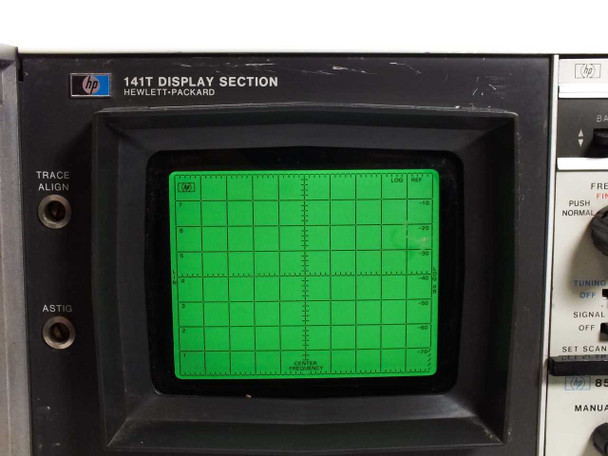
\includegraphics[width=0.62\textwidth]{Figures/Methodology/HP-Display-Section}
		\caption{HP141T \acrshort{crt} display section.}
		\label{fig:display-section}
	\end{figure}
	
	Secondary objectives include digitizing the operations that were previously executed by physical knobs such as horizontal and vertical scaling of the waveform. This objective can be  as functions in a program that can be called to perform similar task. The choice of coding language and available development tools for the program that runs the display is a critical part of the \acrshort{ui} subsystem. 
	
	An alternative approach to handling data acquisition and display functions on the same board would be to use a single-board computer for the display. Spectrum data can be retrieved from memory and displayed to the user in a Python, C/C++ or Java program. Knobs can be replaced by programmatic buttons with functions that users can access by touching the screen. This can allow other features such as averaging and displaying maxima and minima to be easily accessible to the user. For this project, \acrshort{ui} must enable users to select between different display modes, including the \acrshort{phm}, \acrshort{avm} and \acrshort{rwm}. The \acrshort{ui} must enable users to switch between these modes seamlessly and allow for back them to return to previous screens using a back button in the program.
	
	Overall, the project aims to adhere to Nielsen's heuristic design principles which includes:
	\begin{enumerate}
		\item
		Match between the system and the HP141T -  the program should use the language and current features of the HP141T that users are familiar with
		\item 
		User control and freedom - the \acrshort{ui} must support undo, redo and exit points
		\item 
		Aesthetics and minimalist design - the most relevant information that must be displayed is related to the frequency plot of the input signals as well as configurations and settings of the data acquisition and digital processing units that give context to the current display
		\item 
		Flexibility and efficiency of use - the \acrshort{ui} interface of the modernized HP141T must be optimized for difference experience levels through suitable shortcuts and frequent actions such as averaging and showing maxima and minima of the input signal.
		\item 
		Help and documentation - documentation of the modernized HP141T display must correspond to current documentations of the entire system and must be easy to read
		\item 
		Error prevention - the \acrshort{ui} must protect users from deleting stored traces and signal information
		\item 
		Visibility - a user must always know what is happening within the program and current state of their actions
		\item 
		Consistency and standards - the appearance of the \acrshort{ui} must follow the conventions of modern spectrum analyzer displays through consistent words, situations and actions.
		\item 
		Help user to recognize, diagnose and recover from errors such as closing windows with information about pulses or signal noise
		\item 
		Recognition rather than recall - minimize users' memory load by making program features that are related to the most accessed signal data easy to access
	\end{enumerate}
	
	\subsection{Equipment for Debugging and Testing}
	
	The following section gives a review of the project requirement which necessitates the development of an HP141T display emulator of the three auxiliary outputs as shown in \ref{tab:hp141t-output-voltages}. Additionally, the section describes software-based simulation tools that can be used in the development for debugging and obtaining an idea about the expected behaviour individual hardware components and overall system.
	
	\subsubsection{Emulating HP141T Auxiliary Outputs}
	
	The sawtooth signal can be generated using a 555-timer circuit which produces a ramp voltage with adjustable frequency to mimic the adjustable scan time, and a fixed peak-to-peak voltage of $\SI{10}{\volt}$ with no \acrshort{dc} offset. This is to ensure that the horizontal sawtooth output range between $-\SI{5}{\volt}$ and $+\SI{5}{\volt}$ is maintained. 
	
	To emulate the vertical output which swings between $\SI{0}{\volt}$ and $-\SI{0.8}{\volt}$, a simple voltage biasing circuit can be built with appropriate resistor values and input voltage. To control this level, a potentiometer can be used to manually adjust the voltage level within that range. Similarly, the pen-lift output can be produced using a biasing circuit with a potentiometer that allows the voltage to swing between $\SI{0}{\volt}$ and $\SI{14}{\volt}$. 
	
	Lastly, the HP141T display emulator circuit needs to interface with the signal conditioning circuit that prepares the signal voltages to match the operating range of the \acrshort{adc}. Therefore, to avoid the development of multiple circuits, the output cables of the display emulator must be the same as the output cables that take the auxiliary outputs from the HP141T to the signal conditioning circuit.
	
	\subsubsection{Software-Based Simulation Tools}
	
	To optimize the selection and configuration of the data acquisition subsystem, \acrshort{adc}s can be simulated in MATLAB using Simulink to understand the behaviour of the sawtooth input from the HP141T or emulating hardware. Additionally, Simulink provides visualizations of the spectrum of the \acrshort{adc} output which can be used to determine the expected values from sampling signals. Simulink also allows users to add impairments to the \acrshort{adc} for introducing a layer of non-linearity that may be seen for signals with frequencies that are close the edges of the \acrshort{rbw} or intermediate frequency. 
	
	Electronic circuits, such as the signal conditioning circuits with op-amps and level-shifters, can be simulated using LTSpice to predict the expected behaviour. Output values from LTSpice simulations can be used to simulate the behaviour of the system using Simulink with MATLAB.
	\clearpage		
	\section{System Design}
	
	Design decisions in formulating the specifications were informed by the requirement review in the previous section. This section aims to give a full description of the system and the interfaces between the different subsystems. The section begins with a visual representation of the system using a block diagram. Following the visual representation of the design, the section includes specifications and concludes with acceptance and integration tests. 
	
	\subsection{Overview System Block Diagram}
	
	The system block diagram shown in Figure \ref{fig:overall-system-block-diagram} below is a graphical overview of the different stages that an RF signal goes through before the amplitude vs frequency graph is displayed. The modernized HP141T maintains the basic analog signal processing functionality performed by the HP8555A \acrshort{rf} section and the HP8552B \acrshort{if} sections. The scope of the proposed design does not involve any changes to the signal processing components of the plug-in sections. However, the Signal Conditioning Subsystem (\acrshort{scs}) prepares the three auxiliary outputs from the HP552B \acrshort{if} section for the Data Acquisition Subsystem (\acrshort{das}) which requires input voltages in the range between $\SI{0}{\volt}$ and $\SI{3.3}{\volt}$. 	
	
	\begin{figure}
	 	\centering
	 	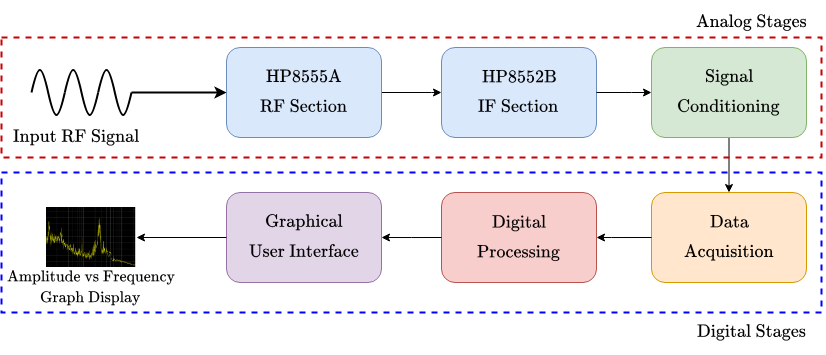
\includegraphics[width=0.65\textwidth]{Figures/Methodology/overall-system-diagram}
	 	\caption{Overview system block diagram for the modernized HP141T which employs the HP8555A and HP8552B plug-in sections.}
	 	\label{fig:overall-system-block-diagram}
	 \end{figure}
 
	\acrshort{adc}s in the \acrshort{das} play a primary role in digitizing the HP141T system by converting the conditioned analog signals into digital values which can be processed in the Digital Processing Subsystem (\acrshort{dps}) which enables manipulation of the digital values. This is particularly necessary for averaging and executing other arithmetic operations in order to satisfy the needs of the user. The Graphical User Interface Subsystem (\acrshort{guis}) manages the display and user preferences for displaying the amplitude vs frequency information of the input \acrshort{rf} signal.
		
	Overall, the can be modularized into five primary subsystems, including:
	\begin{enumerate}
		\item 
		HP141T Subsystem
		\item 
		Signal Conditioning (\acrshort{scs})
		\item 
		Data Acquisition (\acrshort{das})
		\item 
		Digital Processing (\acrshort{dps})
		\item 
		Graphical User Inferface (\acrshort{guis})
	\end{enumerate}
	
	Although this project does not involve the redesign of the HP141T subsystem, an HP141T Emulator design is proposed for simulating the outputs of the \acrshort{if} plug-in section. In particular, the emulator produces signals that are similar to the horizontal, vertical and pen lift outputs of the HP8552B plug-in. This implies that the emulator can be considered as a secondary subsystem that can substitute the HP141T subsystem during calibration of the digital section of the proposed design, as illustrated in figure \ref{fig:emulated-system-diagram}. Furthermore, the diagram illustrates that the emulator does not have high frequency input signals like the HP8555A \acrshort{rf} section plug-in. Instead, oscillators and function generator chips are proposed for producing outputs that approximate the auxiliary outputs, as shown in table \ref{tab:hp8552b-output-vals}.
	
	\begin{figure}[ht!]
		\centering
		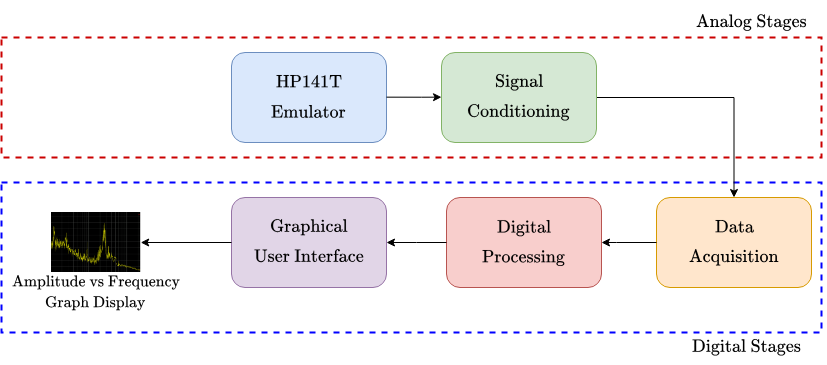
\includegraphics[width=0.65\textwidth]{Figures/Methodology/emulated-system-diagram}
		\caption{Calibration system diagram where the HP141T Emulator is used to configure the primary subsystems such as the \acrshort{scs}, \acrshort{das}, etc.}
		\label{fig:emulated-system-diagram}
	\end{figure}

	All analog stages are executed in \acrshort{pcb}s, and the digital stages are performed by a microcontroller and single-board computer. The following sections detail the specifications of the system modularization and components.

	\subsection{System Modularization}
	
	The system block diagram is expanded as illustrated in figure \ref{fig:system-block-diagram} where the primary components of each of the subsystems are shown. In the diagram, arrows with a solid line illustrate interfaces between subsystems, while arrows with dotted lines describes the flow of analog or digital signals within each subsystem.  
	\begin{figure}
		\centering
		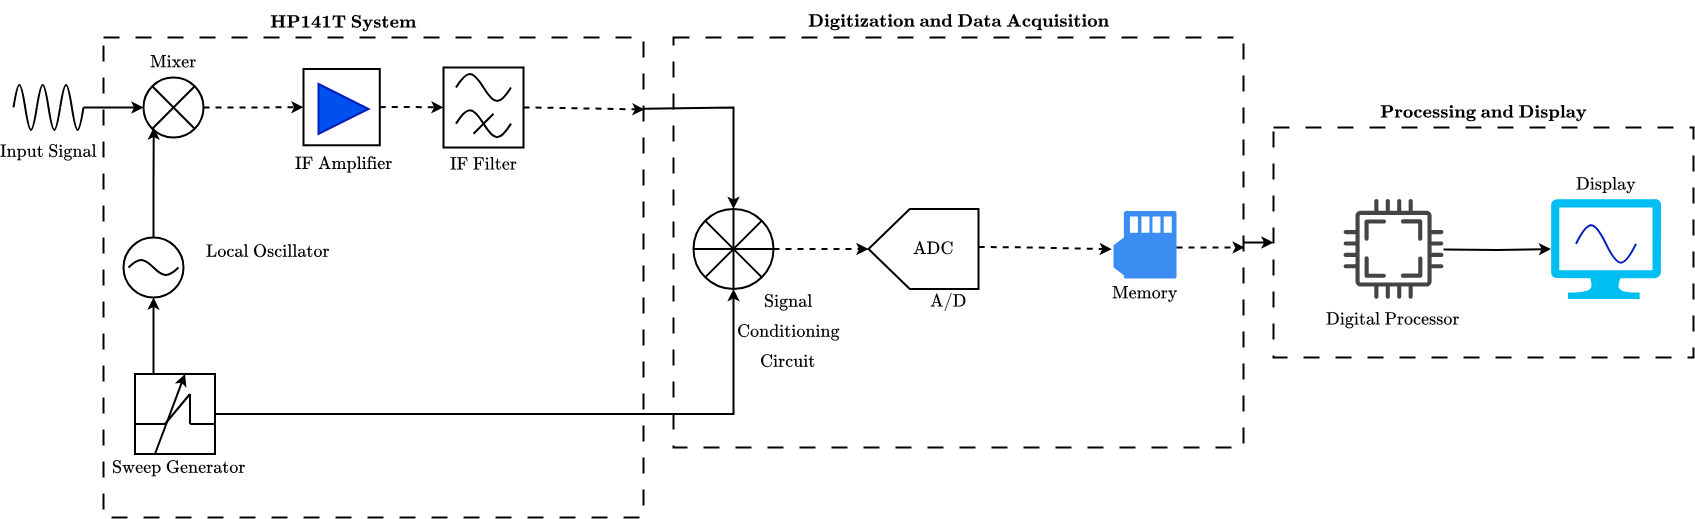
\includegraphics[width=0.90\textwidth]{Figures/Methodology/system-block-diagram}
		\caption{Expansion of the overall system diagram showing the primary components and functions in each subsystem.}
		\label{fig:system-block-diagram}
	\end{figure}

	\begin{table}[ht!]
		\centering
		\label{tab:subsystem-components}
		\begin{tabular}{|m{18em}|m{15em}|m{8em}|}
			\hline
			\cellcolor{cyan!25}\textbf{Subsystem}	& \cellcolor{cyan!25}\textbf{Component}	& \cellcolor{cyan!25}\textbf{Signal Type}\\
			\hline
			\multirow{2}{*}{\textbf{HP141T Subsystem}}	& HP8555A	& Analog\\
			\cline{2-3}
														& HP8552B	& Analog\\
			\hline
			\multirow{3}{*}{\textbf{HP141T Emulator}}	& Vertical Output Simulator	& Analog\\
			\cline{2-3}
														& Horizontal Output Simulator & Analog\\
			\cline{2-3}
														& Pen Lift Output Simulator	& Analog\\
			\hline
			\multirow{3}{*}{\textbf{\acrlong{scs}}}	& Op-amp based vertical output conditioning circuit													& Analog\\
			\cline{2-3}
														& Op-amp based horizontal output conditioning circuit		& Analog\\
			\cline{2-3}
														& Op-amp based pen-lift output conditioning circuit 	& Analog\\
			\hline
			\multirow{3}{*}{\textbf{\acrlong{das}}}	& \acrshort{adc} & Analog/Digital\\
			\cline{2-3}
														& \acrshort{mcu} & Digital\\
			\cline{2-3}
														& Storage Device & Digital\\
			\hline
			\multirow{2}{*}{\textbf{\acrlong{dps}}}	& \acrshort{mcu} & Digital\\
			\cline{2-3}
														& \acrshort{sbc} & Digital\\
			\hline
			\multirow{3}{*}{\textbf{\acrlong{guis}}}	& \acrshort{sbc} & Digital\\
			\cline{2-3}
														& LCD Touch Screen & Digital/Analog\\
			\cline{2-3}
														& Software library & Digital \\
			\hline
		\end{tabular}
		\caption{Showing components in each subsystem and the type of signals that are processed by each unit.}
	\end{table}

	Figure \ref{fig:system-block-diagram} is accompanied by table \ref{tab:subsystem-components} showing subsystem components in more detail. The table also details the components of the HP141T Emulator subsystem. Signal types are noted in table \ref{tab:subsystem-components} because a significant part of the system behaviour can be attributed to the interchange between continuous or discrete values. 
	
	\subsubsection{HP141T Subsystem Specifications}
	
	Table \ref{tab:hp8552b-output-vals} shows the expected outputs collected from the technical manual of the plug-in which also details the expected frequency range. 
	\begin{table}[ht!]
		\centering
		\label{tab:hp8552b-output-vals}
		\begin{tabular}{|c|c|c|c|}
			\hline
			\cellcolor{cyan!25}\textbf{Output}	& \cellcolor{cyan!25}\textbf{Symbol}& \cellcolor{cyan!25}\textbf{Voltage Range}	& \cellcolor{cyan!25}\textbf{Bandwidth} \\
			\hline
			Horizontal & $\texttt{V}_\texttt{x}$	& $-\SI{5.0}{\volt}$ to $\SI{+5.0}{\volt}$	& $\SI{0.005}{\hertz}$ to $\SI{500}{\hertz}$\\
			\hline
			Vertical & $\texttt{V}_\texttt{y}$	& $-\SI{0.8}{\volt}$ to $\SI{0}{\volt}$	& $\SI{10}{\hertz}$ to $\SI{300}{\kilo\hertz}$\\
			\hline
			Pen Lift & $\texttt{V}_\texttt{z}$  & $\SI{0}{\volt}$ to $\SI{14}{\volt}$  & $\SI{0}{\hertz}$\\
			\hline
		\end{tabular}
		\caption{Characteristic values of the HP8552B \acrshort{if} plug-in section's analog output signals \cite{hp8552b}.}
	\end{table}

	Table \ref{tab:hp8552b-amplitude-specs} shows the amplitude specifications of the HP8552B plug-in section. 
	
	\begin{table}[ht!]
		\centering
		\label{tab:hp8552b-amplitude-specs}
		\begin{tabular}{|m{8em}|m{10em}|m{8em}|m{8em}|}
			\hline
			\cellcolor{cyan!25}\textbf{Operation Mode}	& \cellcolor{cyan!25}\textbf{Amplitude Calibration Range} & \cellcolor{cyan!25}\textbf{Amplitude per Division} ($\si{\decibel}$/div)	& \cellcolor{cyan!25}\textbf{Display Range} ($\si{\decibel}$)\\
			\hline
			Logarithmic & $-\SI{130}{\decibel}\text{m}$	to $+\SI{10}{\decibel}\text{m}$ & 10 & 70	\\
			\hline
			Linear & $-\SI{23}{\decibel\volt}$	to $+\SI{117}{\decibel\volt}$ 	& 10 & 70\\
			\hline
		\end{tabular}
		\caption{Amplitude specifications of HP8552B plug-in section \cite{hp8552b}.}
	\end{table}

	The HP8552B has four operational scan modes as shown in table \ref{tab:scan-specifications}. The table also shows the scan time specifications of the HP8552B. 
	
	\begin{table}[ht!]
		\centering
		\label{tab:scan-specifications}
		\begin{tabular}{|c|c|}
			\hline
			\cellcolor{cyan!25}\textbf{Scan Characteristic}	& \cellcolor{cyan!25}\textbf{Description} \\
			\hline
			Scan Time	& 16 scan rates from $\SI{0.1}{\milli\second}/\text{div}$ to $\SI{10}{\second}/\text{div}$ in a 1, 2, 5 sequence\\
			\hline
			\multirow{2}{*}{Scan Time Accuracy} & $\pm10\%$ for scan rates from $\SI{0.1}{\milli\second}/\text{div}$ to $\SI{20}{\milli\second}/\text{div}$\\
			\cline{2-2}
												& $\pm20\%$ for scan rates from $\SI{50}{\milli\second}/\text{div}$ to $\SI{10}{\second}/\text{div}$\\
			\hline
			\multirow{4}{*}{Scan Mode}	& \textit{Internal mode} for repetitive scanning by internally generated ramp	\\
			\cline{2-2}
										& \textit{Single mode} actuated by panel push button\\
			\cline{2-2}
										& \textit{External mode} determined by a $0$ to $+\SI{8}{\volt}$ external signal\\
			\cline{2-2}
										& \textit{Manual mode} controls the scan by the position of the manual knob\\
			\hline
			\multirow{4}{*}{Scan Trigger}	& \textit{Auto trigger} runs the scan freely\\
			\cline{2-2}
											&  \textit{Line trigger} synchronizes the scan with the power line frequency\\
			\cline{2-2}
											& \textit{External trigger} synchronizes the scan with an external signal ($\SI{20}{\volt}$ max) \\
			\cline{2-2}
											& \textit{Video trigger} synchronizes the scan to an envelope of the \acrshort{rf} input signal\\ 
			\hline
		\end{tabular}
		\caption{Scan time and scan mode specifications of the HP8552B plug-in \cite{hp8552b}.}
	\end{table}
		
	\subsubsection{HP141T Emulator Subsystem Design}
	
	According to UR10, the outputs of the HP141T emulator subsystem must simulate the three outputs of the HP8552B \acrshort{if} plug-in section as described in table \ref{tab:user-requirements}. To satisfy this requirement, the HP141T emulator subsystem follows the system diagram illustrated in figure \ref{fig:hp141t-emulator-subsystem-diagram} where a XR2206 is used as a function generator for producing the vertical output, sawtooth scan output corresponding to the horizontal output, and the \texttt{pen up} or \texttt{pen down} state of the pen-lift output. 
	
	\begin{figure}[ht!]
		\centering
		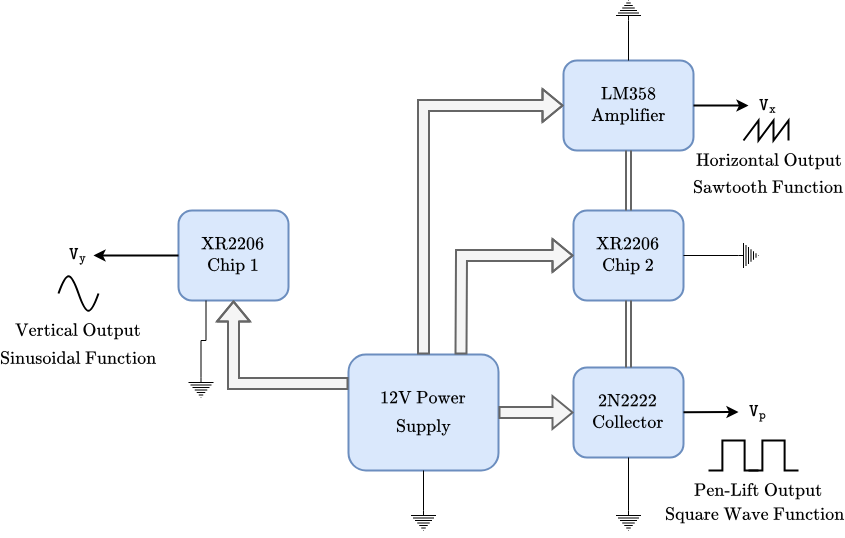
\includegraphics[width=0.60\textwidth]{Figures/Methodology/hp141t-emulator-subsystem-diagram}
		\caption{The HP141T Emulator subsystem diagram showing the primary components powered by the same $\pm\SI{12}{\volt}$ DC dual rail supply.}
		\label{fig:hp141t-emulator-subsystem-diagram}
	\end{figure}
	
	The frequency range of the $\SI{-0.8}{\volt}-\SI{0}{\volt}$ vertical output, $\texttt{V}_\texttt{y}$, is limited to the bandwidth of the video filter in the \acrshort{if} section, i.e. $\SI{10}{\hertz}$ to $\SI{300}{\kilo\hertz}$ \cite{hp8552b}. The front panel check procedure in the technical manual of the HP8552B \acrshort{if} section sets a frequency range of up to $\SI{10}{\kilo\hertz}$ in the video filter, corresponding to a $\SI{30}{\mega\hertz}$ fundamental signal at the input of the \acrshort{rf} section plug-in \cite{HP8555A}.  
	
	\begin{figure}[h!]
		\centering
		\begin{subfigure}{.5\textwidth}
			\centering
			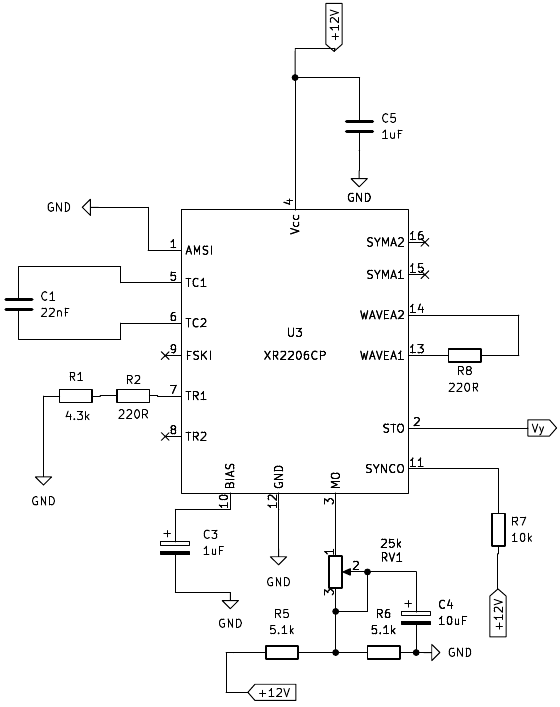
\includegraphics[width=.8\linewidth]{Figures/Methodology/hp8552b-vertical-output-emulator-3}
			\caption{Vertical output emulator circuit.}
			\label{fig:vertical-output-emulator-ct-a}
		\end{subfigure}%
		\begin{subfigure}{.5\textwidth}
			\centering
			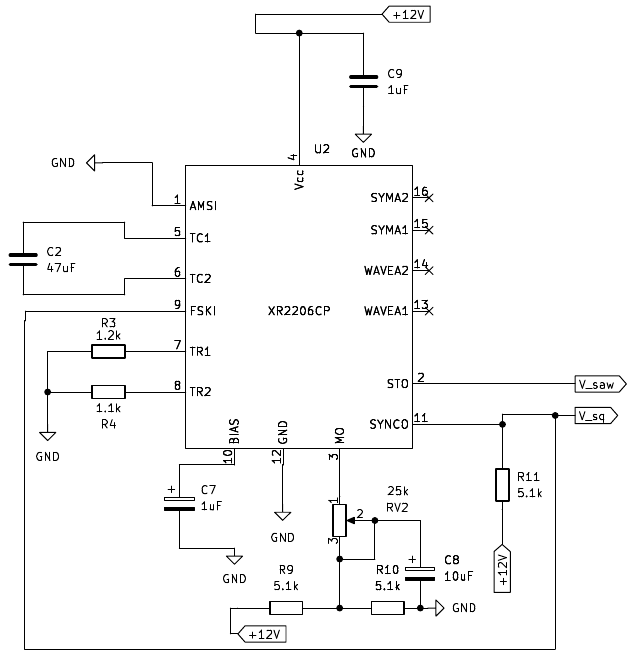
\includegraphics[width=.8\linewidth]{Figures/Methodology/hp8552b-horizontal-output-emulator-3}
			\caption{Horizontal output emulator circuit.}
			\label{fig:horizontal-output-emulator-ct-a}
		\end{subfigure}
		\caption{Emulator circuits for vertical and horizontal outputs of the HP8552B \acrshort{if} section.}
		\label{fig:hp8552B-vh-emulator}
	\end{figure}
	
	Two XR2206 functional generator chips are implemented for emulating the HP8552B outputs, $\texttt{V}_\texttt{y}$ and $\texttt{V}_\texttt{x}$. For $\texttt{V}_\texttt{y}$, timing resistors and capacitors are employed to emulate video filter output during the configuration procedure described in the chip's datasheet which implements a sinusoidal wave with a calibration frequency of $\SI{10}{\kilo\hertz}$, corresponding to a $\SI{30}{\mega\hertz}$ RF signal at the input of the HP8555A plug-in. The full vertical output simulator circuit is illustrated in figure \ref{fig:vertical-output-emulator-ct-a}, adopted from the recommended configuration \cite{xr2206}. The expected shape and time domain characteristics of the $3~\text{V}_\text{pp}$ sinusoidal wave are shown in figure \ref{fig:emulator-vertical-output-sinewave}. 
	
		
	The required frequency is produced by an internal voltage-controlled oscillator that is set by a timing resistor at pin 7 and 8. Pin descriptions and the values of the capacitors and resistors that are connected to them are recorded in table \ref{tab:voec-pin-description} and \ref{tab:vertical-output-emulator-ct-specifications}.
	
%	\begin{table}[ht!]
%		\caption{Pin connection description for the XR2206-based vertical output simulation circuit.}
%		\label{tab:voec-pin-description}
%		\centering
%		\begin{tabular}{|m{3em}|c|c|m{10em}|m{18em}|}
%			\hline
%			\cellcolor{cyan!25}\textbf{Pin No.} & \cellcolor{cyan!25}\textbf{Type}	& \cellcolor{cyan!25}\textbf{Symbol} & \cellcolor{cyan!25}\textbf{Connection(s)} & \cellcolor{cyan!25}\textbf{Description} \\
%			\hline
%			1	&	I	& AMSI 	&	GND  & A $\SI{0}{\volt}$ amplitude modulation signal input.\\
%			\hline
%			2	&   O	& STO	&	$\texttt{V}_\texttt{y}$ & Sinusoid wave output.\\
%			\hline
%			3	& 	O	& MO	&	C8, RV2, R17, R18		& Multiplier output for controlling the amplitude of $\texttt{V}_\texttt{y}$\\
%			\hline
%			4	& 	I	& $\text{V}_{\text{CC}}$ & C7 & $+\SI{12}{\volt}$ power supply with decoupling capacitor.\\
%			\hline
%			5	& 	I	& TC1	&	C5			 & Timing capacitor.\\
%			\hline
%			6	&	I	& TC2	& 	C5			 & Timing capacitor.\\
%			\hline
%			7	&	O	& TR1	&	R15, R16	 & Timing resistor.\\
%			\hline
%			8	&	X	& TR2	&	X			 & No connection.\\
%			\hline
%			9	&	X	& FSKI	&	X			 & No connection.\\  
%			\hline
%			10	&	O	& BIAS	&	C6			 & Internal voltage reference.\\
%			\hline
%			11	&	O	& SYNCO	&	R20			 & Open collector with a pull-up resistor to the power
%			supply.\\
%			\hline
%			12	& 		& GND	&	GND			 & Ground pin.\\
%			\hline
%			13	&	I	& WAVEA1	&	R19		 & First waveform-adjustment input.\\
%			\hline
%			14	&	I	& WAVEA2	&	R19		 & Second waveform-adjustment input.\\
%			\hline
%			15	&	X	& SYMA1		&	X		 & No connection for wave symmetry adjustment.\\
%			\hline
%			16	&	X	& SYMA2		&	X		 & No connection for wave symmetry adjustment.\\
%			\hline
%		\end{tabular}
%	\end{table}

	\begin{table}[ht!]
		\caption{Pin connection description for the XR2206-based vertical output simulation circuit.}
		\label{tab:voec-pin-description}
		\centering
		\begin{tabular}{|m{3em}|c|m{10em}|m{18em}|}
			\hline
			\cellcolor{cyan!25}\textbf{Pin No.} & \cellcolor{cyan!25}\textbf{Type}	& \cellcolor{cyan!25}\textbf{Symbol} & \cellcolor{cyan!25}\textbf{Description} \\
			\hline
			1	&	I	& AMSI 	& A $\SI{0}{\volt}$ amplitude modulation signal input.\\
			\hline
			2	&   O	& STO	&	Sinusoid wave output.\\
			\hline
			3	& 	O	& MO	&	Multiplier output for controlling the amplitude of $\texttt{V}_\texttt{y}$\\
			\hline
			4	& 	I	& $\text{V}_{\text{CC}}$ & $+\SI{12}{\volt}$ power supply with decoupling capacitor.\\
			\hline
			5	& 	I	& TC1	&	Timing capacitor.\\
			\hline
			6	&	I	& TC2	& 	Timing capacitor.\\
			\hline
			7	&	O	& TR1	&	Timing resistor.\\
			\hline
			8	&	X	& TR2	&	 No connection.\\
			\hline
			9	&	X	& FSKI	&	No connection.\\  
			\hline
			10	&	O	& BIAS	&	 Internal voltage reference.\\
			\hline
			11	&	O	& SYNCO	&	 Open collector with a pull-up resistor to the power
			supply.\\
			\hline
			12	& 		& GND		& Ground pin.\\
			\hline
			13	&	I	& WAVEA1	&	 First waveform-adjustment input.\\
			\hline
			14	&	I	& WAVEA2	&	Second waveform-adjustment input.\\
			\hline
			15	&	X	& SYMA1		&	 No connection for wave symmetry adjustment.\\
			\hline
			16	&	X	& SYMA2		&	 No connection for wave symmetry adjustment.\\
			\hline
		\end{tabular}
	\end{table}
	The amplitude of $\texttt{V}_\texttt{y}$ and $\texttt{V}_\texttt{x}$ at the output of the XR2206 chips is controlled by adjusting the variable resistors $\text{RV1}$ and $\text{RV2}$ and limited to $0$.
	\begin{figure}[ht!]
		\centering
		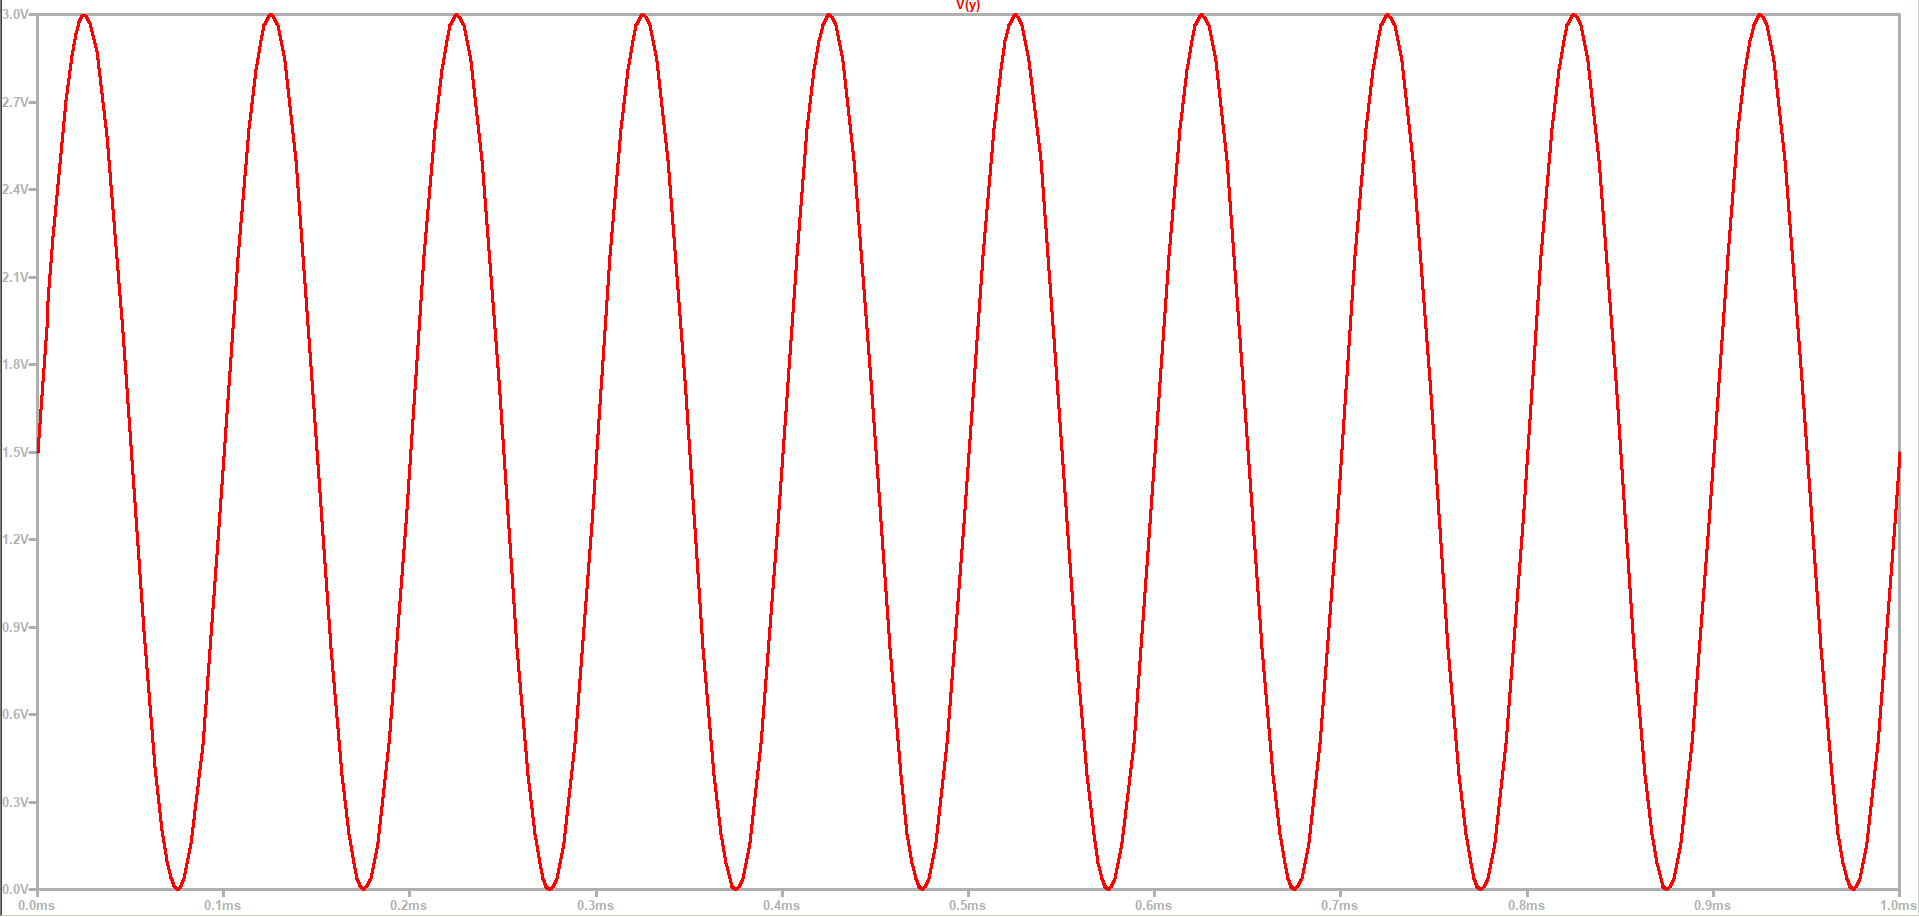
\includegraphics[width=0.50\textwidth]{Figures/Methodology/emulator-vertical-output-sinewave}
		\caption{Simulated output at the STO pin of the XR2206 chip employed in emulating the vertical output of as a $3~\text{V}_\text{pp}$ sinusoidal wave.}
		\label{fig:emulator-vertical-output-sinewave}
	\end{figure}
	To generate a sinusoid with a constant peak-to-peak voltage and constant frequency for the vertical output, an external capacitance of $\text{C} = \text{C}_1$ is connected across pin 5 and 6, and a timing resistance $\text{R} = \text{R}_1 + \text{R}_2$ across pin 7, such that the operational frequency $\texttt{f}_\texttt{y}$ of the XR2206 is 
	\begin{align}\label{eqn:xr2206-sinewave-frequency}
		\text{f}_\texttt{y}	& = \frac{1}{\text{R}\text{C}} ~ [\si{\hertz}]
	\end{align}
	Similarly, the characteristics of the horizontal sawtooth output depend on the timing components at pin 5, 6, and 7, as illustrated in figure \ref{fig:horizontal-output-emulator-ct-a}. However, when operating as a sawtooth function generator as in the case of the horizontal output emulator circuit, the frequency $\texttt{f}_y$ is given by,
	\begin{align}\label{eqn:xr2206-sawtooth-frequency}
		\text{f}_\texttt{x}	& = \frac{2}{\text{C}(\text{R}_a + \text{R}_b)} ~ [\si{\hertz}]
	\end{align}
	where $\text{R}_a$ and $\text{R}_b$ correspond to the timing resistors connected to pin 7 and pin 8, and $\text{C}$ is the timing capacitor connected to pin 5 and pin 6, respectively. The duty cycle of the output sawtooth function is given by the parallel combination of $\text{R}_a$ and $\text{R}_b$, such that 
	\begin{align}\label{eqn:xr2206-duty-cycle}
		\text{Duty Cycle}	& = \frac{\text{R}_a}{\text{R}_a + \text{R}_b}
	\end{align}
	The design associates a duty cycle with the proportion of time that the signal spends rising from the minimum voltage to the maximum of the sawtooth function in the output of the emulator, i.e. as the XR2206 STO output voltage increases from the $\SI{0}{\volt}$ to $\SI{3}{\volt}$. The design approximates the rise time, $\text{t}_\text{rise}$, and duty cycle of this output from the manual of the HP8552B as illustrated in figure \ref{fig:hp8552b-sawtooth} \cite{hp8552b}. Using $\text{R}_a = \text{R}_3 = \SI{1.1}{\kilo\ohm}$ and $\text{R}_b = \text{R}_4 = \SI{1.2}{\kilo\ohm}$, the duty cycle is approximated to $52.2\%$ and the rise time to $\SI{54}{\milli\second}$. These time domain characteristics correspond to a horizontal oscillation frequency of $\SI{18.52}{\second}$, given that the timing capacitance is $\SI{47}{\micro\farad}$. 
	\begin{table}[ht!]
		\caption{HP141T emulator electrical specifications.}
		\label{tab:vertical-output-emulator-ct-specifications}
		\centering
		\begin{tabular}{|cm{10em}m{5em}m{5em}m{5em}m{8em}|}
			\hline
			\cellcolor{cyan!25}\textbf{Designation} & \cellcolor{cyan!25}\textbf{Parameter} &	\cellcolor{cyan!25}\textbf{Minimum} &  \cellcolor{cyan!25}\textbf{Maximum}	& \cellcolor{cyan!25}\textbf{Units} & \cellcolor{cyan!25}\textbf{Conditions}\\
			\hline
			\multicolumn{6}{c}{\textbf{General Characteristics}}\\
			\hline
			$\text{V}_{\text{IN}}$ & Split Supply Voltage  & $9$ & $12$ & $\si{\volt}$ & \\
			\hline
			$\text{I}_{\text{IN}}$ & Supply Current  & $12$ & $17$ & $\si{\milli\ampere}$ & \\
			\hline
			\multicolumn{6}{c}{\textbf{Output Voltage Characteristics}}\\
			\hline
			$\texttt{V}_\texttt{y}$	& Vertical Output	&	$0$	&	$3$ & $\si{\volt}$ & $\text{RV1} = \SI{25}{\kilo\ohm}$ \\
			\hline
			$\texttt{V}_\texttt{x}$	& Horizontal Output	&	$-4.75$	&	$4.76$ & $\si{\volt}$ & $\text{RV2} = \SI{15}{\kilo\ohm}$\\
			\hline
			$\texttt{V}_\texttt{p}$	& Pen Lift Output	&   $0$	& 	$12$ & $\si{\volt}$ & \\
			\hline
			\multicolumn{6}{c}{\textbf{Frequency and Time Domain Characteristics}}\\
			\hline
			$\text{f}_\texttt{y}$	& Vertical Output Oscillation Frequency	&	&	$10$ & $\si{\kilo\hertz}$ & $\text{R}_1 = \SI{4.3}{\kilo\ohm}$, $\text{R}_2 = \SI{220}{\ohm}$, $\text{C}_1 = \SI{22}{\micro\farad}$ \\
			\hline
			$\text{f}_\texttt{x}$	& Horizontal Output Frequency	& $17.24$ 	& $20$ & $\si{\hertz}$ & $\text{R}_3 = \SI{1.2}{\kilo\ohm}$, $\text{R}_4 = \SI{1.3}{\ohm}$, $\text{C}_2 = \SI{47}{\micro\farad}$\\
			\hline
			$\text{t}_\text{rise}$				& Horizontal Output Sawtooth Rise Time	& $50$	&	$58$ &	$\si{\milli\second}$	&	$\text{R}_3 = \SI{1.2}{\kilo\ohm}$, $\text{R}_4 = \SI{1.3}{\ohm}$, $\text{C}_2 = \SI{47}{\micro\farad}$\\
			\hline
			$\text{T}_\texttt{x}$	&	Sawtooth Period	& $95.6$	& $111$	& $\si{\milli\second}$	& \\
			\hline
		\end{tabular}
	\end{table}
	\begin{figure}[ht!]
		\centering
		
\includegraphics[width=0.34\textwidth]{Figures/Methodology/hp8552b-sawtooth}
		\caption{Illustration of the duty cycle and rise time of sawtooth function corresponding to the horizontal output, $\texttt{V}_\texttt{x}$, of the HP8552B.}
		\label{fig:hp8552b-sawtooth}
	\end{figure}
	
	Since the output voltage of the multiplier and wave shaper in the XR2206 is limited between $\SI{0}{\volt}$ to $\SI{3}{\volt}$, the circuit in figure \ref{fig:emulator-circuit-level-shift} is used to adjust the sawtooth output from the chip to rise from $-\SI{5}{\volt}$ to $+\SI{5}{\volt}$.
	
	\begin{figure}[ht!]
		\centering
		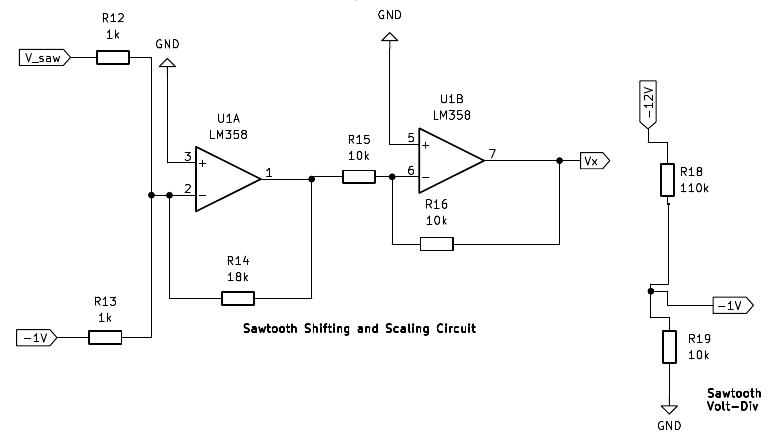
\includegraphics[width=0.50\textwidth]{Figures/Methodology/hp8552b-horizontal-output-level-shifter-3}
		\caption{XR2206 sawtooth output level shifter for achieving the appropriate voltage range.}
		\label{fig:emulator-circuit-level-shift}
	\end{figure}
	The sawtooth output of the XR2206 circuit is simulated in LTSpice using the \texttt{PWL} command as shown in figure \ref{fig:sawtooth-sim-ltspice}, with the corresponding results of the simulation shown in the figure \ref{fig:sawtooth-sim-output}. The \texttt{PWL} command simulates a piecewise function between time $t_1$ and $t_n$, $\text{n}\geq 2$. The simulation shows that the expected voltage range of the scan output lies between $-\SI{4.75}{\volt}$ and $\SI{4.76}{\volt}$ with a steep rise time and a clipped voltage at $\SI{4.76}{\volt}$. The simulation also indicates a start time delay in the output. This is due to the capacitors in the LM358 op-amp which introduce RC time constants during discharge. This delay, steep rise time, and voltage clipping of the sawtooth is accounted for and adjustment are made in software, as specified in the following sections. 
	
	\begin{figure}[ht!]
		\centering
		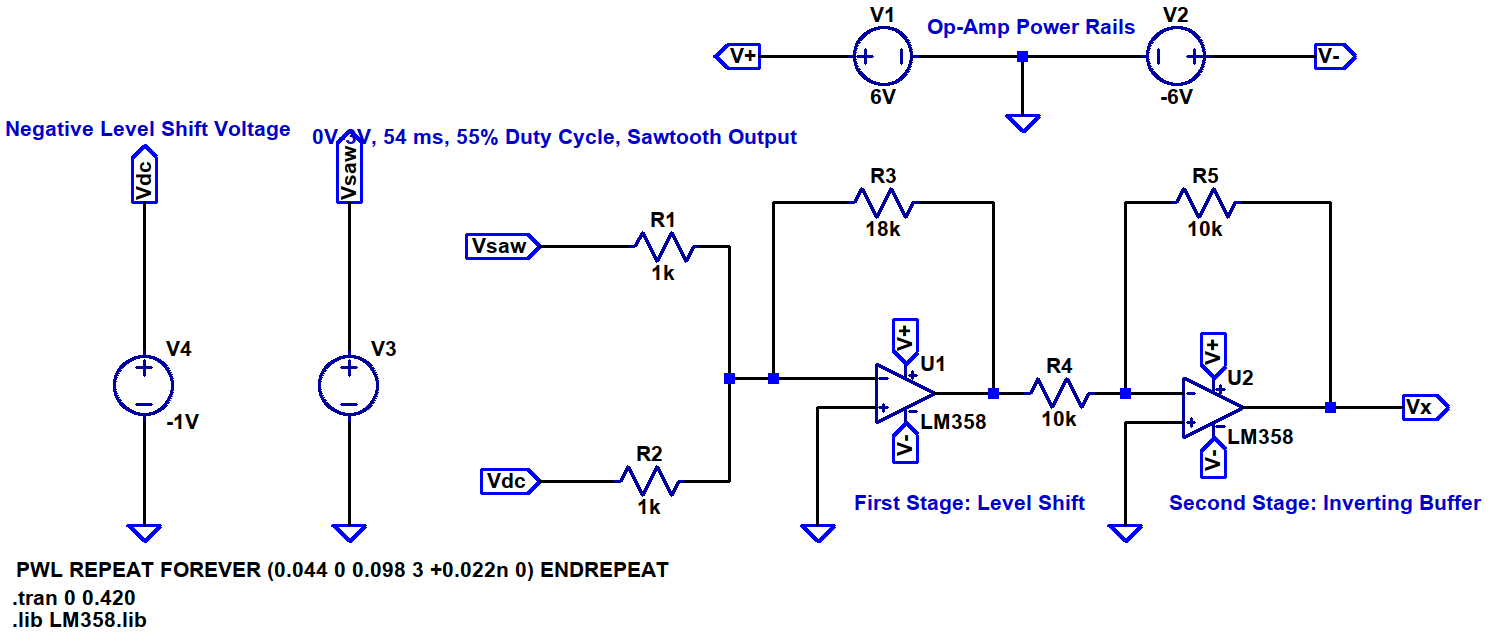
\includegraphics[width=0.65\linewidth]{Figures/Methodology/emulator-triangle-shift-ct-sim-1}
		\caption{Simulated level shift circuit.}
		\label{fig:sawtooth-sim-ltspice}
	\end{figure}

	The first stage of the level shifting and scaling circuit in figure \ref{fig:emulator-circuit-level-shift} and \ref{fig:sawtooth-sim-ltspice} using an LM358 op-amp as a difference amplifier with a gain of $18$ to scale the sawtooth voltage, in the range between $\SI{0}{\volt}$ and $\SI{3}{\volt}$, to the desired range from $-\SI{5}{\volt}$ to $+\SI{5}{\volt}$. The second stage is an inverting buffer which serves to invert the output of the first stage such that the gradient of the sawtooth increases in the same direction. 

	\begin{figure}
		\centering
		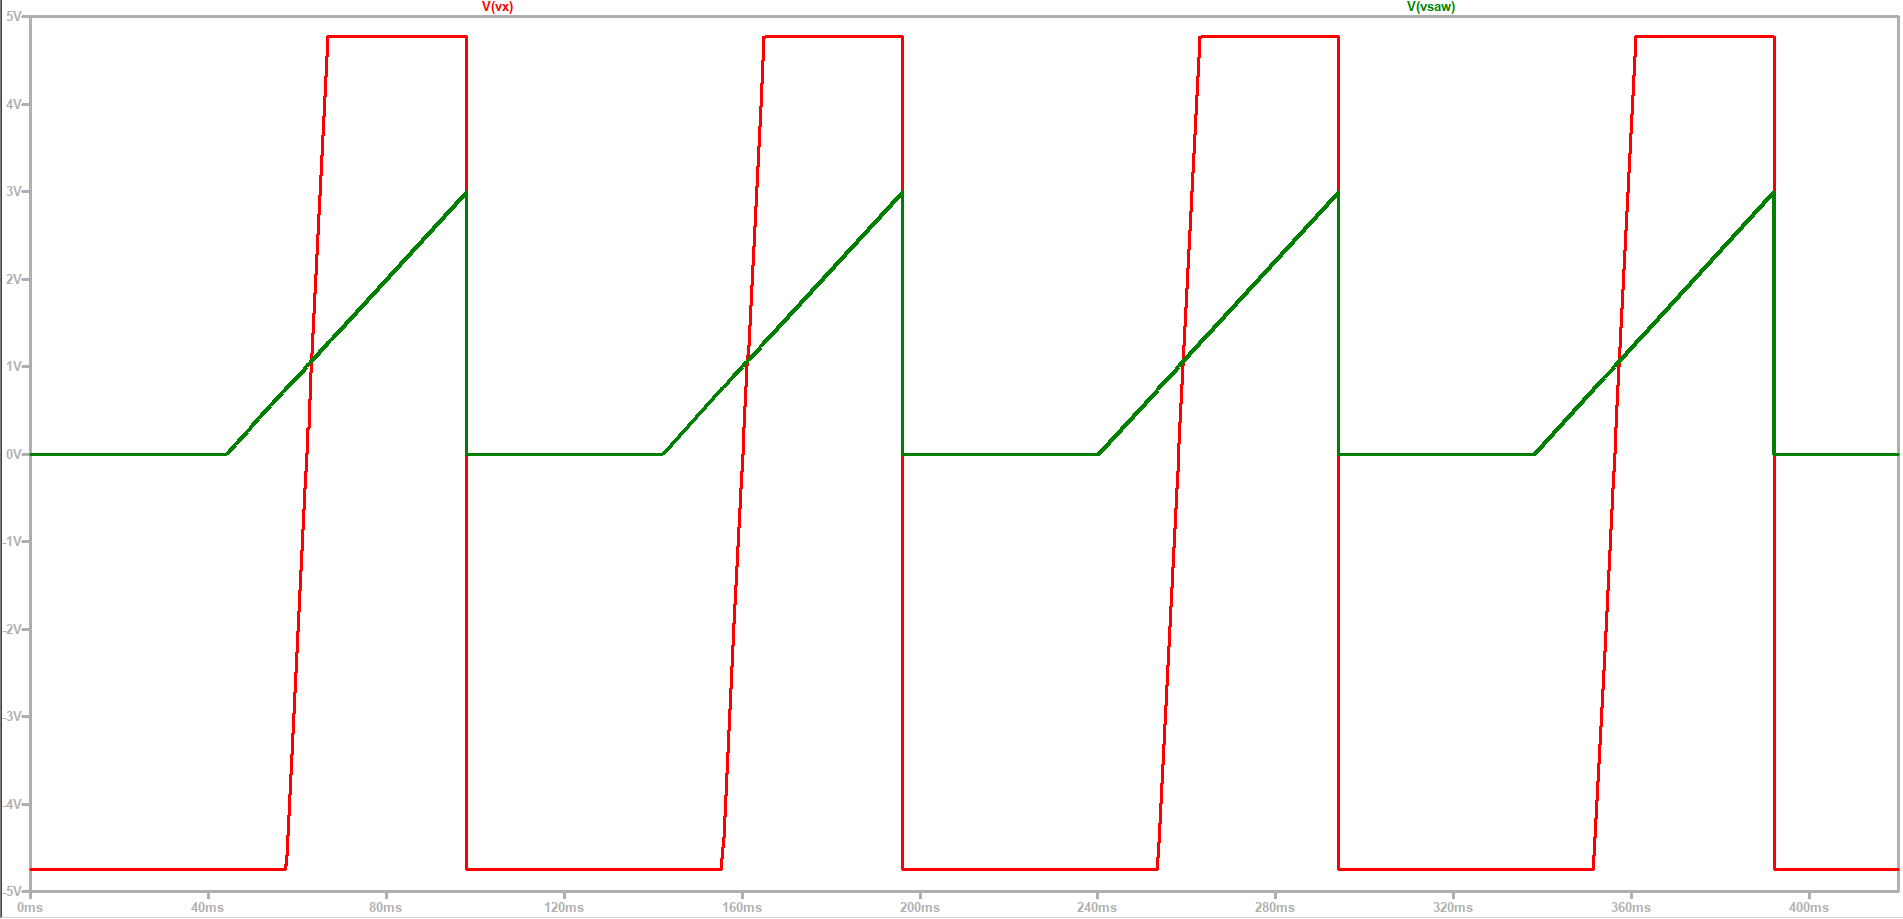
\includegraphics[width=0.7\linewidth]{Figures/Methodology/emulator-sawtooth-output-1}
		\caption{Showing simulated scan output of the emulator.}
		\label{fig:sawtooth-sim-output}
	\end{figure}

	The period in the simulated sawtooth remains the same, however, the duty cycle decreases due to the delay and shorter rise time of the output, as seen in figure \ref{fig:sawtooth-sim-output}. The duty cycle is scaled from $52.2\%$ to $40.9\%$ while the start time of the output is delayed by $\SI{18}{\milli\second}$ and the rise time is scaled from $\SI{54}{\milli\second}$ to $\SI{10}{\milli\second}$, indicating a time scaling factor of 5.4. The start time of the output signal is delayed by $\SI{13}{\milli\second}$ from the start time of the XR2206 STO output. The software accounts for the time scaling, delay and change in the duty cycle to ensure accurate simulation of the rise time of $\SI{54}{\milli\second}$. 
	
	\begin{figure}
		\centering
		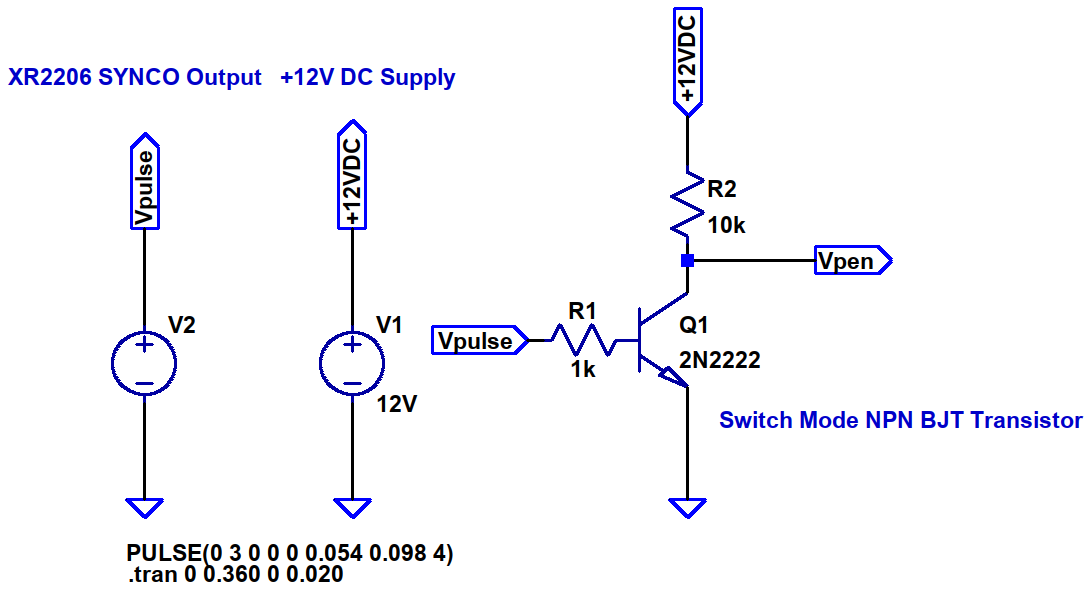
\includegraphics[width=0.45\linewidth]{Figures/Methodology/emulator-pen-lift-ct-sim}
		\caption{Simulation of the pen lift output using the XR2206 SYNCO pulse output.}
		\label{fig:emulator-pen-lift-ct-sim}
	\end{figure}
	
	\begin{figure}
		\centering
		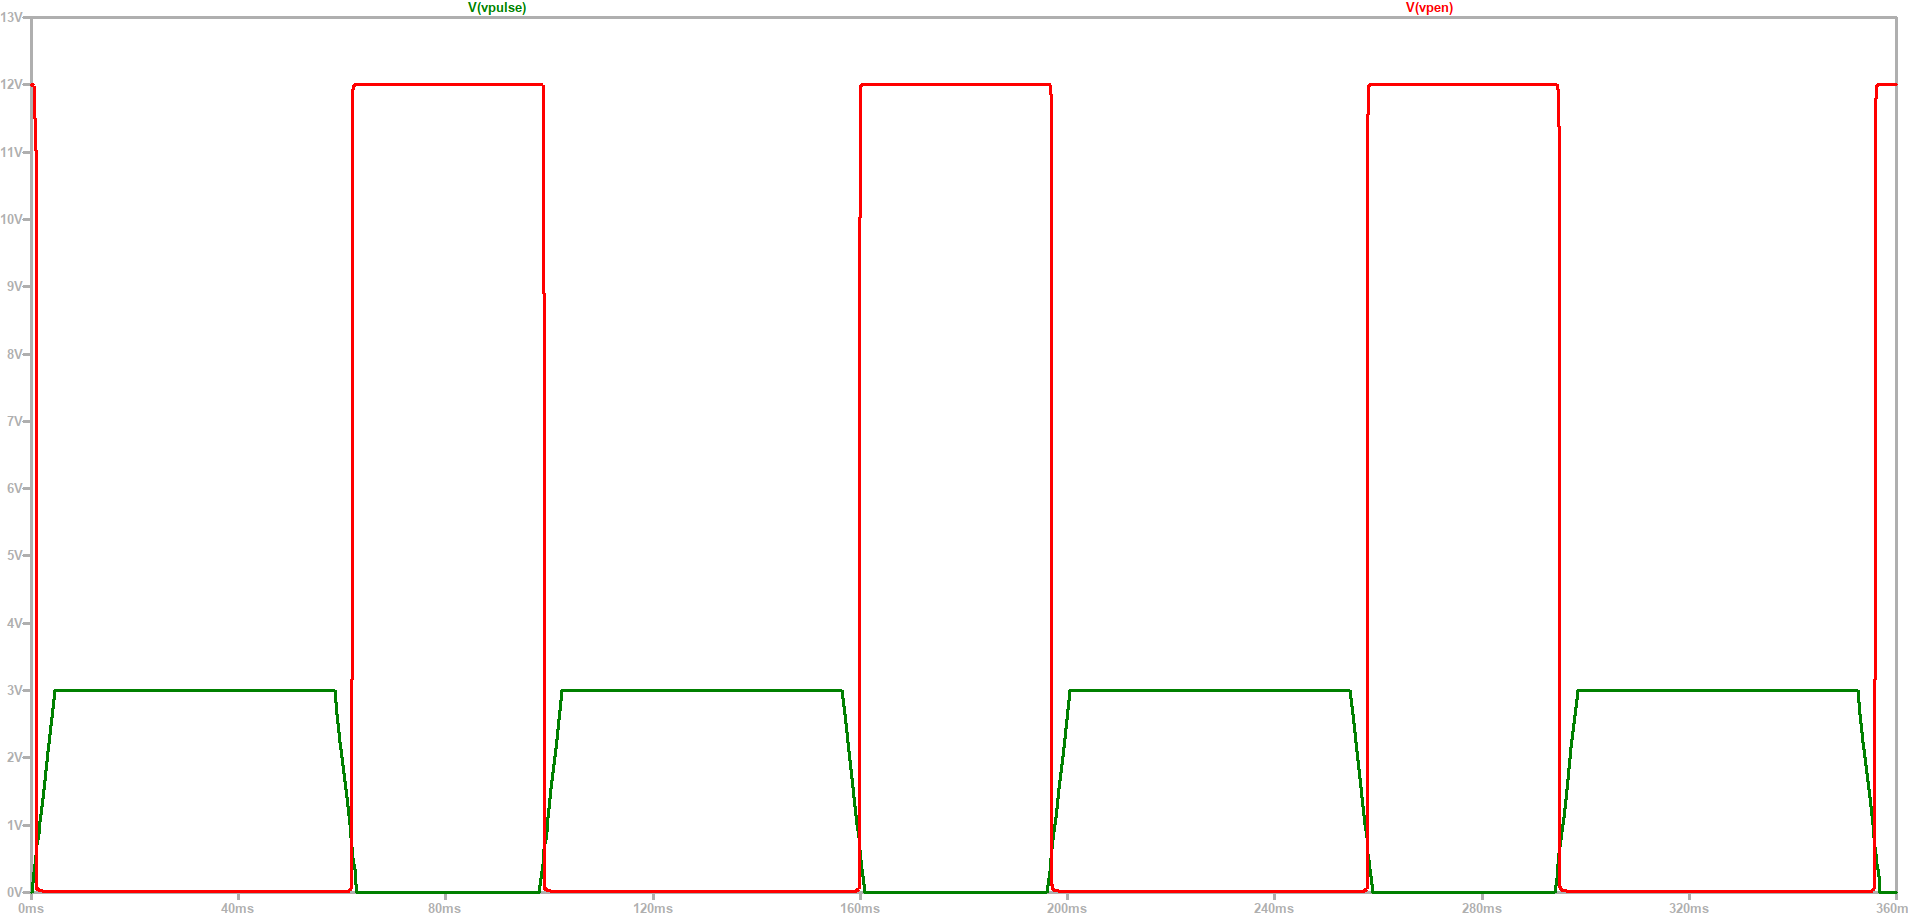
\includegraphics[width=0.7\linewidth]{Figures/Methodology/emulator-pen-lift-ct-sim-output}
		\caption{Pen lift output simulation with the XR2206 SYNCO pulse in green and the pulse at the collector of the NPN transistor in red.}
		\label{fig:emulator-pen-lift-ct-output}
	\end{figure}

	The states of the pen-lift output are produced using a square wave pulse at the SYNCO pin output of the XR2206 chip. The SYNCO pulse has the same duty cycle and period as the sawtooth output at the STO pin. Ideally, this allows for the design to synchronise the pen-lift output states with the scan time. A 2N2222 NPN transistors is employed as a switch such that the collector voltage goes high ($\SI{12}{\volt}$) when the SYNCO pulse is off, as shown in figure \ref{fig:emulator-pen-lift-ct-output}. In other words, when the collector output is high, the pen-lift output is in the \texttt{pen down} state. Conversely, when the collector output is low, the pen-lift output is in the \texttt{pen up} state. The implications of these states on the display are discussed in detail in section \ref{subsec:display}. 
	
	\begin{table}[h!]
		\centering
		\label{tab:emulator-pen-lift-specs}
		\begin{tabular}{cccccc}
			\hline
			\cellcolor{cyan!25}\textbf{Designation} & \cellcolor{cyan!25}\textbf{Parameter} & \cellcolor{cyan!25}\textbf{Minimum} & \cellcolor{cyan!25}\textbf{Maximum} & \cellcolor{cyan!25}\textbf{Units} &  \cellcolor{cyan!25}\textbf{Condition}\\
			\hline
			$\text{V}_\text{B}$	& Base input voltage & $0$ & $3$ & $\si{\volt}$ & $\text{R}_\text{B} = \SI{1}{\kilo\ohm}$\\ 
			\hline
			$\text{V}_\text{C}$ & Collector output voltage & $0$ & $12$ & $\si{\volt}$ & $\text{R}_\text{C} = \SI{10}{\kilo\ohm}$\\
			\hline
			$\text{V}_\text{E}$ & Emitter voltage & $0$ &	& $\si{\volt}$ &  \\
			\hline
		\end{tabular}
		\caption{Specifications of the pen lift circuit as part of the HP141T emulator subsystem based on the 2N2222 NPN transistor.}
	\end{table}

	A simulation of the XR2206 SYNCO square wave and pen-lift output is shown in figure \ref{fig:emulator-pen-lift-ct-sim} where the \texttt{PULSE} command is used in LTSpice. The base and collector boltages of the NPN transistor, and other specifications, are included in table \ref{tab:emulator-pen-lift-specs}. The table corresponds to the simulation output where the transistor turns on and pulls the collector voltage to $\SI{0}{\volt}$ when the SYNCO square wave is high ($\SI{3}{\volt}$). When the square wave is low ($\SI{0}{\volt}$), the transistor turns of and the collector output is pulled up to $\SI{12}{\volt}$ through the $\SI{10}{\kilo\ohm}$ resistor.  
	
	\begin{figure}[h!]
		\centering
		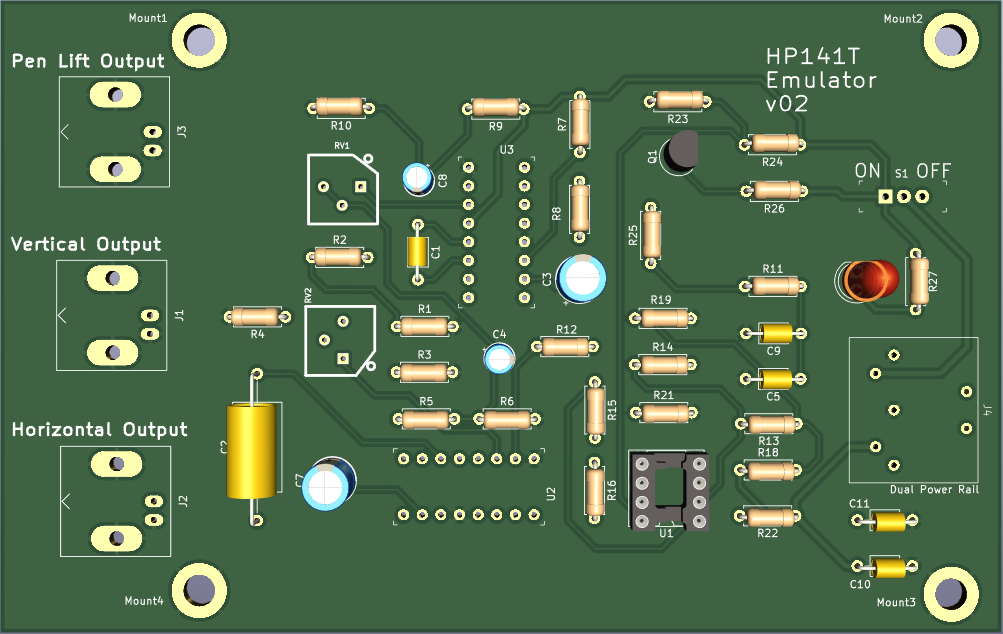
\includegraphics[width=0.5\linewidth]{Figures/Methodology/emulator-pcb-3d-front-v03}
		\caption{3D view of the HP141T Emulator subsystem's \acrshort{pcb}.}
		\label{fig:emulator-pcb}
	\end{figure}
	
	The full HP141T Emulator subsystem is implemented on a \acrshort{pcb} as illustrated in the 3D model in figure \ref{fig:emulator-pcb}. The output of the system is interfaced through a \acrshort{bnc} coaxial cable for its low loss capabilities for improved performance. 
	
	\begin{figure}[h!]
		\centering
		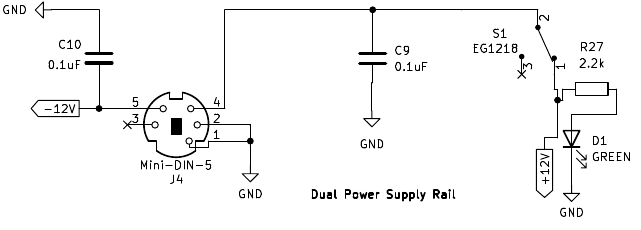
\includegraphics[width=0.55\linewidth]{Figures/Methodology/emulator-power-supply}
		\caption{HP141T Emulator power supply circuit with decoupling capacitors to reduce high frequency noise.}
		\label{fig:emulator-power-ct}
	\end{figure}
	
	A $\SI{28}{\watt}$ power brick that converts $\SI{230}{\volt}$, $\SI{50}{\hertz}$ AC to $\pm\SI{12}{\volt}$ DC dual supply. The power supply is connected to the \acrshort{pcb} through a 5 pole din socket as illustrated in figure \ref{fig:emulator-power-ct}. Decoupling capacitors are used to blocks high frequency noise by creating a high-pass RC filter with the total impedance of the subsystem that smooths any fluctuations in the power supply. The subsystem can be switched on by setting the 3 pole switch to the left-hand position and switched off by setting it to the centre right-hand position. A power LED is used to indicate whether the subsystem is on or off. 
	
	\subsubsection{Signal Conditioning Subsystem Design}
	
	The \acrshort{scs} forms the central part in the digitization and modernization of the HP141T \acrshort{sa} as it interfaces with the HP141T subsystem and HP141T Emulator subsystem through three separate \acrshort{bnc} coaxial cables and prepares the horizontal, vertical and pen-lift outputs to a suitable input voltage range for the unipolar operation STM32H723ZG board, i.e. $\SI{0}{\volt}$ to $\SI{3.3}{\volt}$ DC. This implies that the outputs of the HP8552B \acrshort{if} section or HP141T Emulator are the inputs to the \acrshort{scs} at the \acrshort{bnc} ports  illustrated in figure \ref{fig:sig-cond-bnc-ct-schematic} showing the circuit schematic of the \acrshort{bnc} connector which takes in the vertical output $\texttt{V}_\texttt{y}$. 
	
	\begin{figure}[h!]
		\centering
		\begin{subfigure}{.33\textwidth}
			\centering
			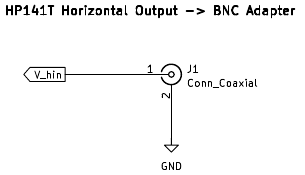
\includegraphics[width=.8\linewidth]{Figures/Methodology/sig-cond-bnc-ct-schematic-j1}
			\caption{Horizontal input $\texttt{V}_\texttt{hin}$.}
			\label{fig:sig-cond-bnc-j1}
		\end{subfigure}
		\begin{subfigure}{.33\textwidth}
			\centering
			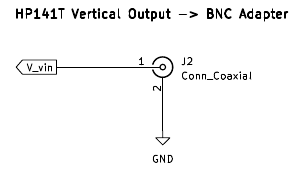
\includegraphics[width=.8\linewidth]{Figures/Methodology/sig-cond-bnc-ct-schematic-j2}
			\caption{Vertical input $\texttt{V}_\texttt{vin}$.}
			\label{fig:sig-cond-bnc-j2}
		\end{subfigure}
		\begin{subfigure}{.33\textwidth}
			\centering
			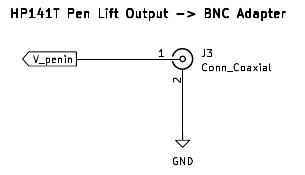
\includegraphics[width=.8\linewidth]{Figures/Methodology/sig-cond-bnc-ct-schematic-j3}
			\caption{Pen-lift input $\texttt{V}_\texttt{penin}$.}
			\label{fig:sig-cond-bnc-j3}
		\end{subfigure}
		\caption{Schematic of the input connectors that enable the \acrshort{scs} to interface with the outputs from the HP8552B plug-in or HP141T Emulator subsystem.}
		\label{fig:sig-cond-bnc-ct-schematic}
	\end{figure}

	Conversion of the input voltages to the appropriate level of $\SI{3.3}{\volt}$ for the analog-to-digital interface employs three LM358 op-amps in different pipeline circuits that apply the required scaling and level shifting for each input. The flow of each input through this pipelined analog subsystem is illustrated in figure \ref{fig:sig-cond-subsystem-diagram}. The circuits in each pipeline share a common GND to reduce noise in the system and ensure that the \acrshort{adc} in the \acrshort{das} produces accurate results.
	
	\begin{figure}[h!]
		\centering
		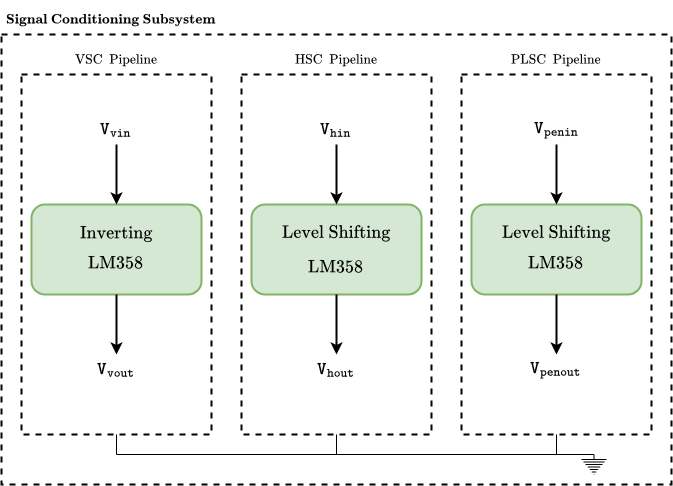
\includegraphics[width=0.55\linewidth]{Figures/Methodology/sig-cond-subsystem-diagram}
		\caption{\acrlong{scs} diagram.}
		\label{fig:sig-cond-subsystem-diagram}
	\end{figure}

	In the \acrfull{hsc} pipeline, the $\texttt{V}_\texttt{hin}$ sawtooth enters the circuit through the \acrshort{bnc} connector and is labelled at the input node as seen in figure \ref{fig:sig-cond-hsc-schematic}. The expected input range is $-\SI{5}{\volt}$ to $\SI{5}{\volt}$ from the auxiliary output of the HP8552B \acrshort{if} section. A $\SI{100}{\kilo\ohm}$ resistance is connected between the non-inverting input (pin 3) of the LM358 op-amp (U1A) in order to set the input impedance and pull the voltage input voltage to $\SI{3.3}{\volt}$. Additional $\SI{68}{\kilo\ohm}$ and $\SI{220}{\kilo\ohm}$ resistances contribute to the amplification as well as establishing a reference voltage at the non-inverting input. 
	
	\begin{figure}[h!]
		\centering
		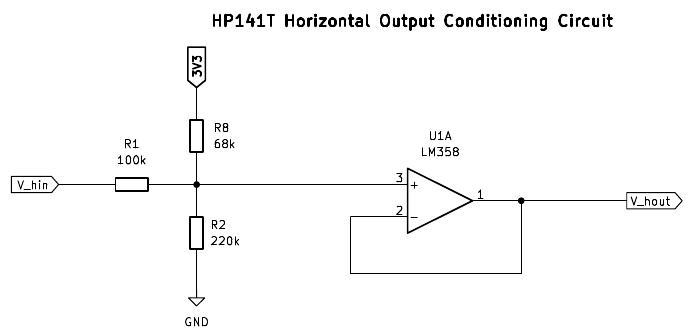
\includegraphics[width=0.55\linewidth]{Figures/Methodology/sig-cond-hsc-schematic}
		\caption{The \acrshort{hsc} pipeline uses an LM358 op-amp to process the horizontal output signal from the HP141T scaling and shifting it to match the sampling microcontroller's \acrshort{adc}'s $\SI{0}{\volt}$ to $\SI{3.3}{\volt}$ input range.}
		\label{fig:sig-cond-hsc-schematic}
	\end{figure}

	The $\SI{0}{\volt}$ to $\SI{3.3}{\volt}$ conditioned output, $\texttt{V}_\texttt{hout}$ is extracted through male connector pins as illustrated in figure \ref{fig:sig-cond-output-schematic}. 
	
	%Schematic of the \acrshort{bnc} connector for receiving the vertical output signal $\texttt{V}_\texttt{y}$ ($\text{V}_\text{vin}$) from the HP8552B plug-in or HP141T Emulator subsystem

	%Since the input voltage range is limited to $\SI{0}{\volt}$ to $\SI{3.3}{\volt}$, the outputs of the \acrshort{scs} are constrained to values within this range. The \acrshort{scs} implements jumper wires to transmit the signals to the \acrshort{adc}s on the STM32H723ZG board. Output connectors of the \acrshort{scs} are illustrated in \ref{fig:sig-cond-output-schematic}. An additional $\SI{3.3}{\volt}$ output is included for debugging and testing purposes. Table \ref{tab:sig-cond-in-out-specs} includes the input/output voltage and current range specifications for the \acrshort{scs}. 
	
	\begin{figure}[h!]
		\centering
		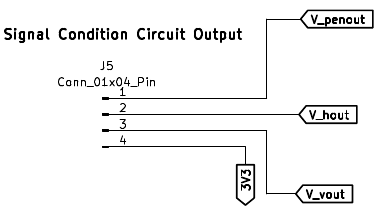
\includegraphics[width=0.35\linewidth]{Figures/Methodology/sig-cond-output-ct-schematic}
		\caption{Circuit schematic of the connectors with $\SI{0}{\volt}$ to $\SI{3.3}{\volt}$ outputs corresponding to the digitized values of the vertical, horizontal, and pen-lift outputs of the \acrshort{scs}.}
		\label{fig:sig-cond-output-schematic}
	\end{figure}
	
	The output of the \acrshort{hsc} pipeline was simulated in LTSpice to determine the expected behaviour of the circuit. The simulation results are included in figure \ref{fig:sig-cond-hsc-sim-output} where the output, in purple, is restricted to the desired input range of the microcontroller's \acrshort{adc}. The simulation was run for $\SI{400}{\milli\second}$ using the \texttt{PWL} command to reproduce the $-\SI{5}{\volt}$ to $\SI{5}{\volt}$ input sawtooth as a piecewise function.  
	
	\begin{figure}[h!]
		\centering
		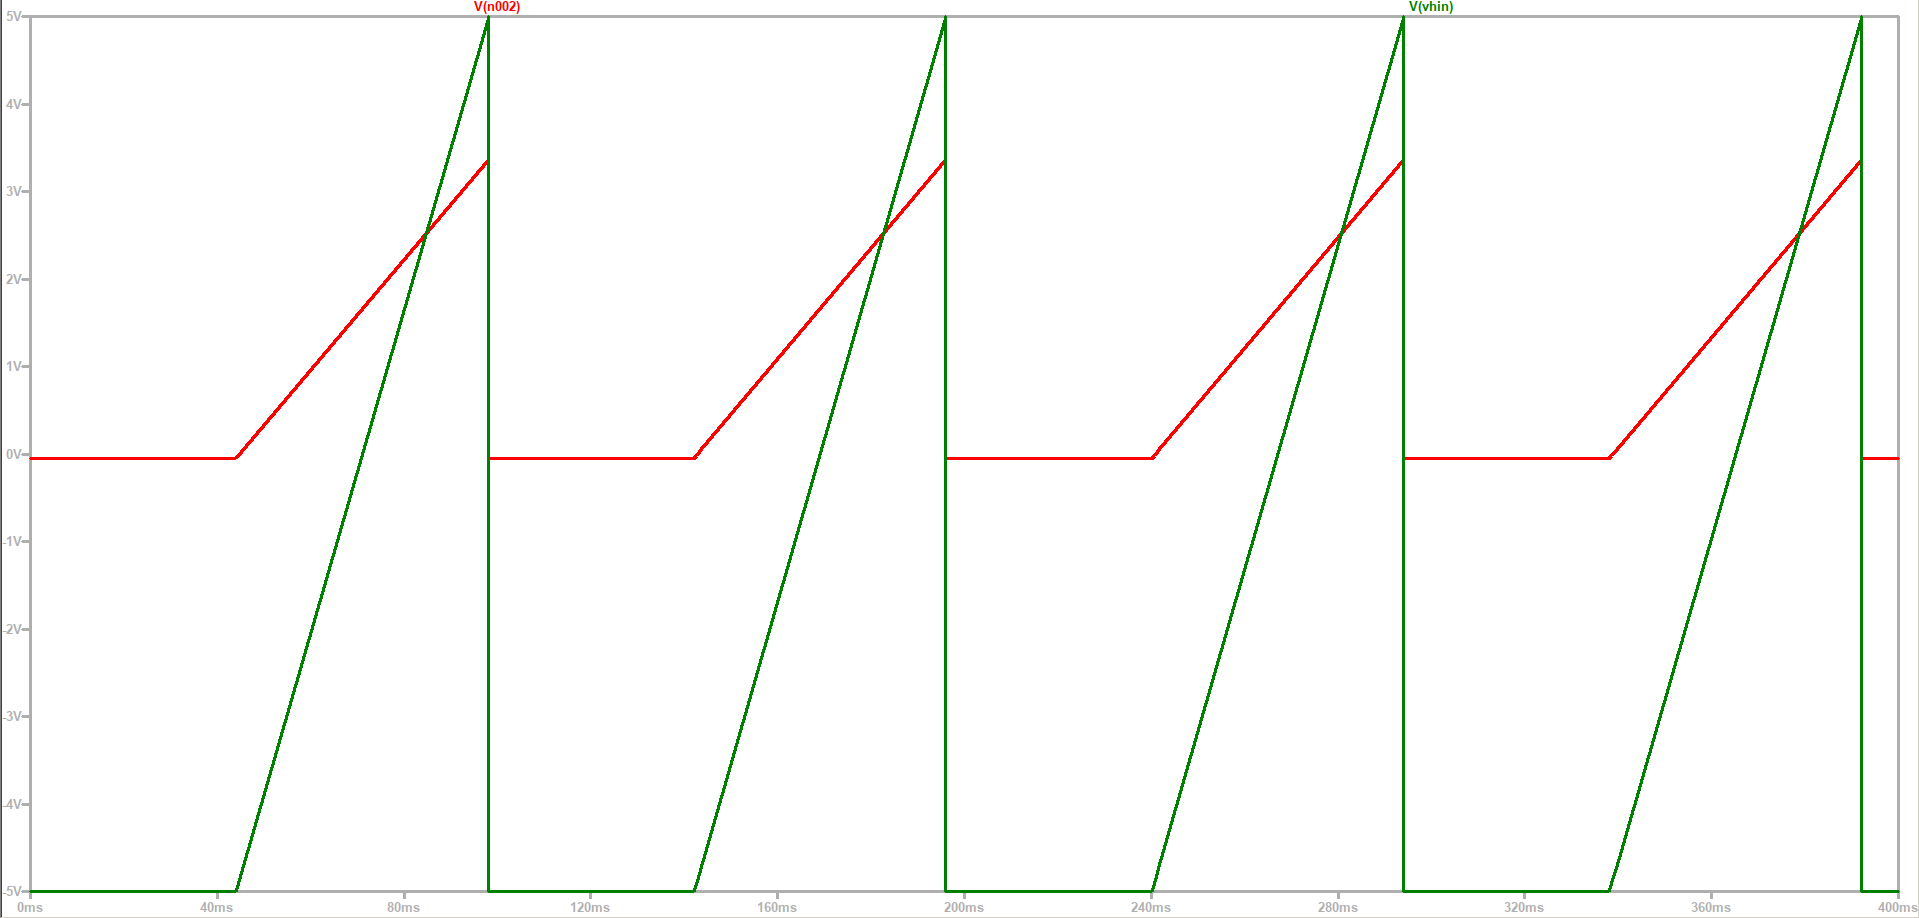
\includegraphics[width=0.7\linewidth]{Figures/Methodology/sig-cond-hsc-sim-output}
		\caption{\acrshort{hsc} simulation output showing that the op-amp configuration is expected to maintain the shape of the sawtooth scan output.}
		\label{fig:sig-cond-hsc-sim-output}
	\end{figure}

	The specifications of the \acrshort{scs} with respect to the \acrshort{hsc} pipeline are summarized in table \ref{tab:sig-cond-hsc-specs}. 
	
	\begin{table}[ht!]
		\centering
		\label{tab:sig-cond-hsc-specs}
		\caption{Input and output specifications of the \acrshort{scs}.}
		\begin{tabular}{ccc}
			
		\end{tabular}
	\end{table}
	
	The vertical output from the HP8552B is conditioned using LM358 op-amps in the inverting amplifier configuration with a gain of $A_{vsc} = -3.7$ using a $\SI{10}{\kilo\ohm}$ feedback resistor and a $\SI{2.7}{\kilo\ohm}$ input resistor. This configuration was selected because the expected input voltage range of the \acrlong{vsc}, $\texttt{V}_\texttt{vin}$, is $-\SI{0.8}{\volt}$ to $\SI{0}{\volt}$, and inverting and amplifying the small, negative voltages, is necessary for the operation of the \acrshort{adc}s on the STM32H723ZG. The \acrshort{vsc} circuit is depicted in figure \ref{fig:sig-cond-vsc-schematic} with a $\SI{2.2}{\kilo\ohm}$ compensating resistor at the non-inverting input of the LM358 op-amp to minimize the contribution of the input offset bias current.
	
	\begin{figure}[h!]
		\centering
		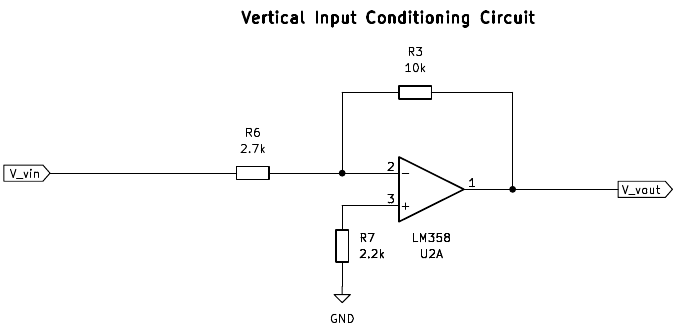
\includegraphics[width=0.7\linewidth]{Figures/Methodology/sig-cond-vsc-schematic}
		\caption{An inverting amplifier configuration is used in the \acrshort{vsc} pipeline to prepare the vertical output of the HP8552B for digital processing.}
		\label{fig:sig-cond-vsc-schematic}
	\end{figure}
	
	The \acrshort{vsc} circuit was simulated for different voltages and frequencies. A sinusoidal function was used in the simulation to model the fluctuations in the vertical output representing deflections in the amplitude of the input. To determine the behaviour of the \acrshort{vsc} with respect to changes in voltage, a control frequency of $\SI{10}{\kilo\hertz}$ was used. This frequency was selected corresponding to the calibration output of the HP8552B. Figure \ref{fig:sig-cond-vsc-sine-sim-output} shows the expected behaviour of the \acrshort{vsc} circuit for a sinusoidal $\texttt{V}_\texttt{vin}$ with a $\SI{0.8}{\volt}_{pp}$ amplitude. The output, $\texttt{V}_\texttt{vout}$, has a global minimum at $\SI{0}{\volt}$ and a global maximum at $\SI{3.0}{\volt}$ which is suitable for the input of the microcontroller's \acrshort{adc}s. The plot shows that the shape of the input signal is maintained at the output, however, the output is out of phase by $\pi\si{\radian}$. In other words, the input is flipped and scaled by the inverting amplifier configuration. 
	
	\begin{figure}[h!]
		\centering
		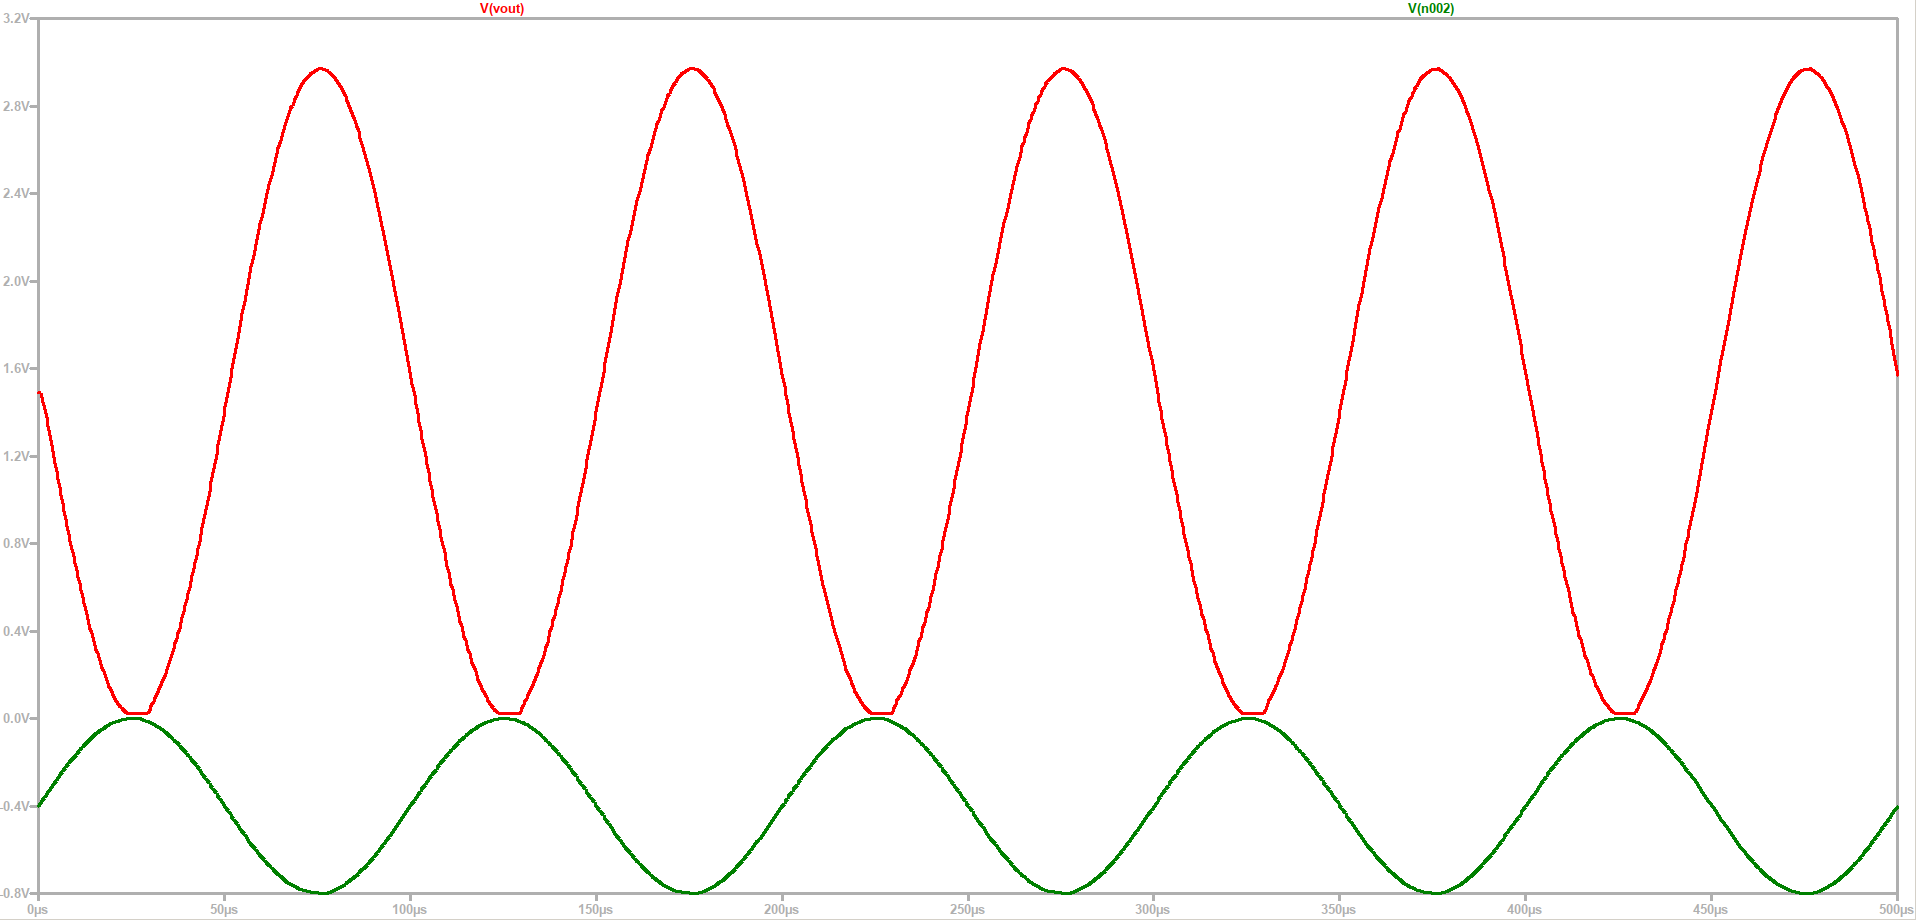
\includegraphics[width=0.7\linewidth]{Figures/Methodology/sig-cond-vsc-sine-sim-output}
		\caption{Simulation output for the case where $\texttt{V}_\texttt{vin}$ assumes all values in the range between $-\SI{0.8}{\volt}$ to $\SI{0}{\volt}$.}
		\label{fig:sig-cond-vsc-sine-sim-output}
	\end{figure} 

	Simulation results show slight distortions in the shape of the output for input voltages starting from $-\SI{0.4}{\volt}$ as shown in figure \ref{fig:sig-cond-vsc-sim-0-4}. The distortions become more apparent for $\texttt{V}_\texttt{vin}$ values that are lower than or equal $-\SI{0.32}{\volt}$ as seen in figure \ref{fig:sig-cond-vsc-sine-sim-0-16Vpp} where the shape of the output is clipped at $\SI{0}{\volt}$. 
	
	\begin{figure}[h!]
		\centering
		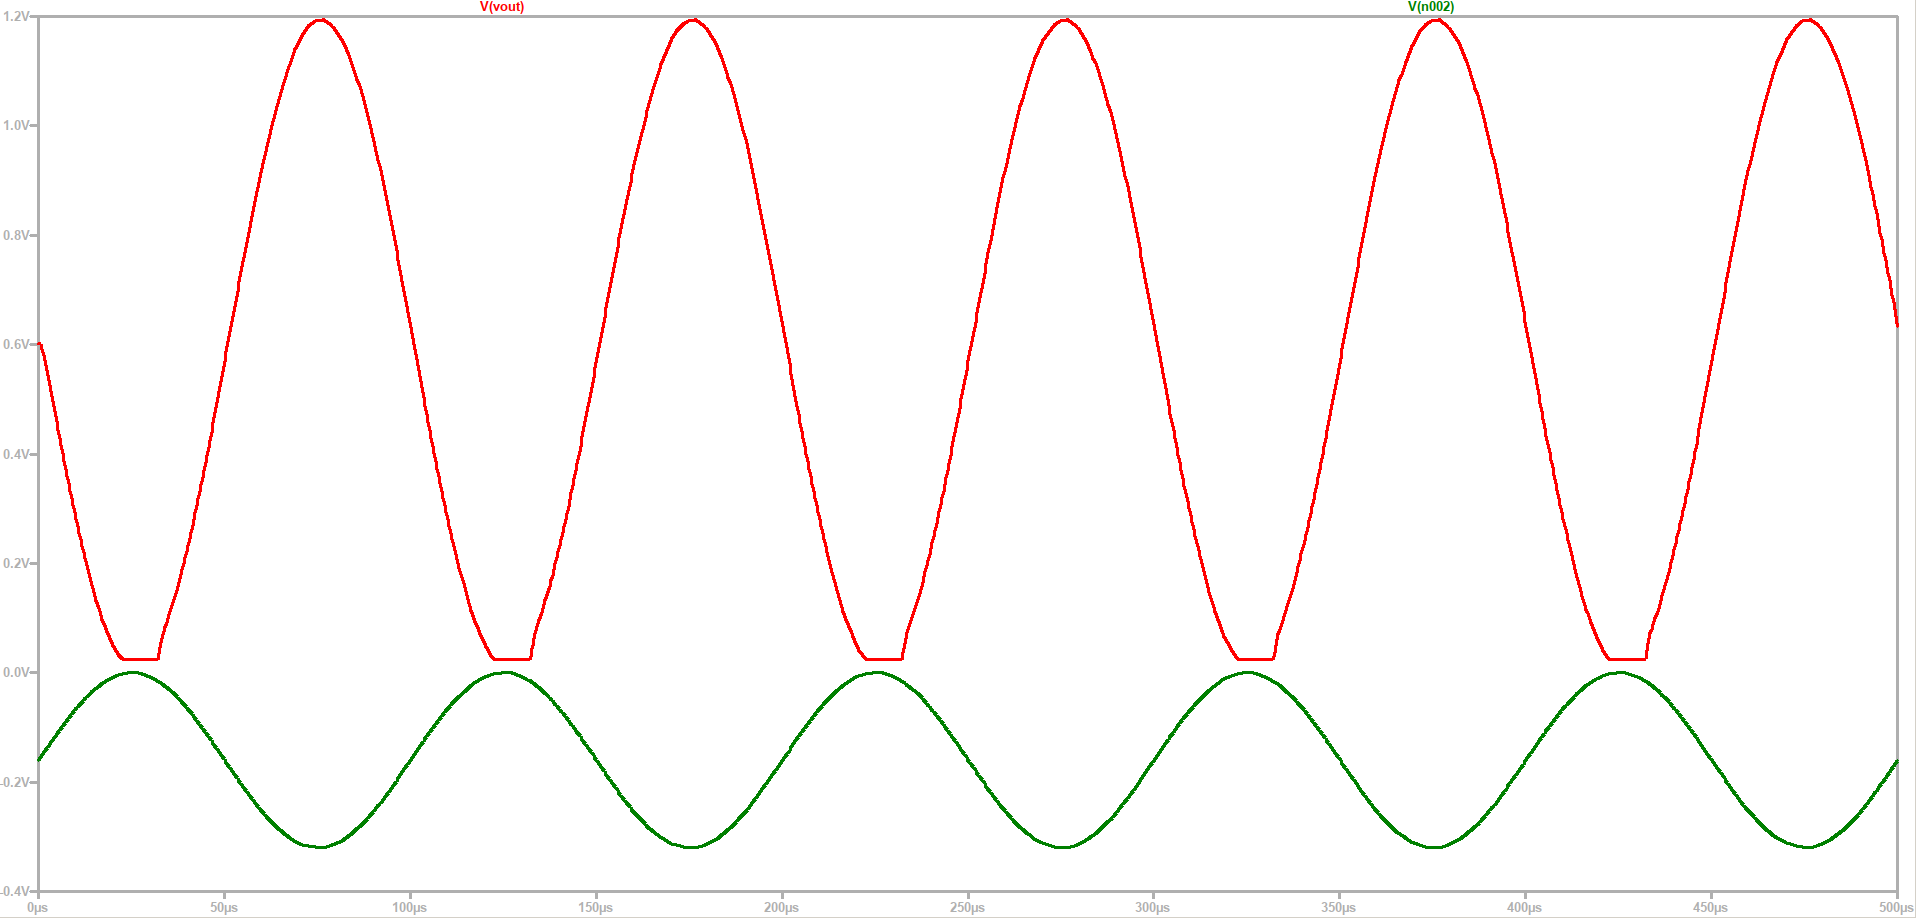
\includegraphics[width=0.7\linewidth]{Figures/Methodology/sig-cond-vsc-sine-sim-output-0-32Vpp}
		\caption{Simulation shows significant clipping of the output at $\SI{0}{\volt}$ when $\texttt{V}_\texttt{vin}$ has a peak-to-peak voltage of $-\SI{0.32}{\volt}$.}
		\label{fig:sig-cond-vsc-sine-sim-0-16Vpp}
	\end{figure}  

	Voltage clipping of the \acrshort{vsc} pipeline output indicates a loss in the accuracy of the amplitude. According to the datasheet, the linear accuracy of the HP8552B in the vertical output is $\SI{0.1}{\micro\volt}$. However, simulations results showed that the sensitivity of the \acrshort{vsc} circuit is $\SI{70}{\micro\volt}$, as seen in figure \ref{fig:sig-cond-vsc-sine-sim-output-0024Vpp}, corresponding to the voltage where visible change in the output start to be seen. 
	
	\begin{figure}[h!]
		\centering
		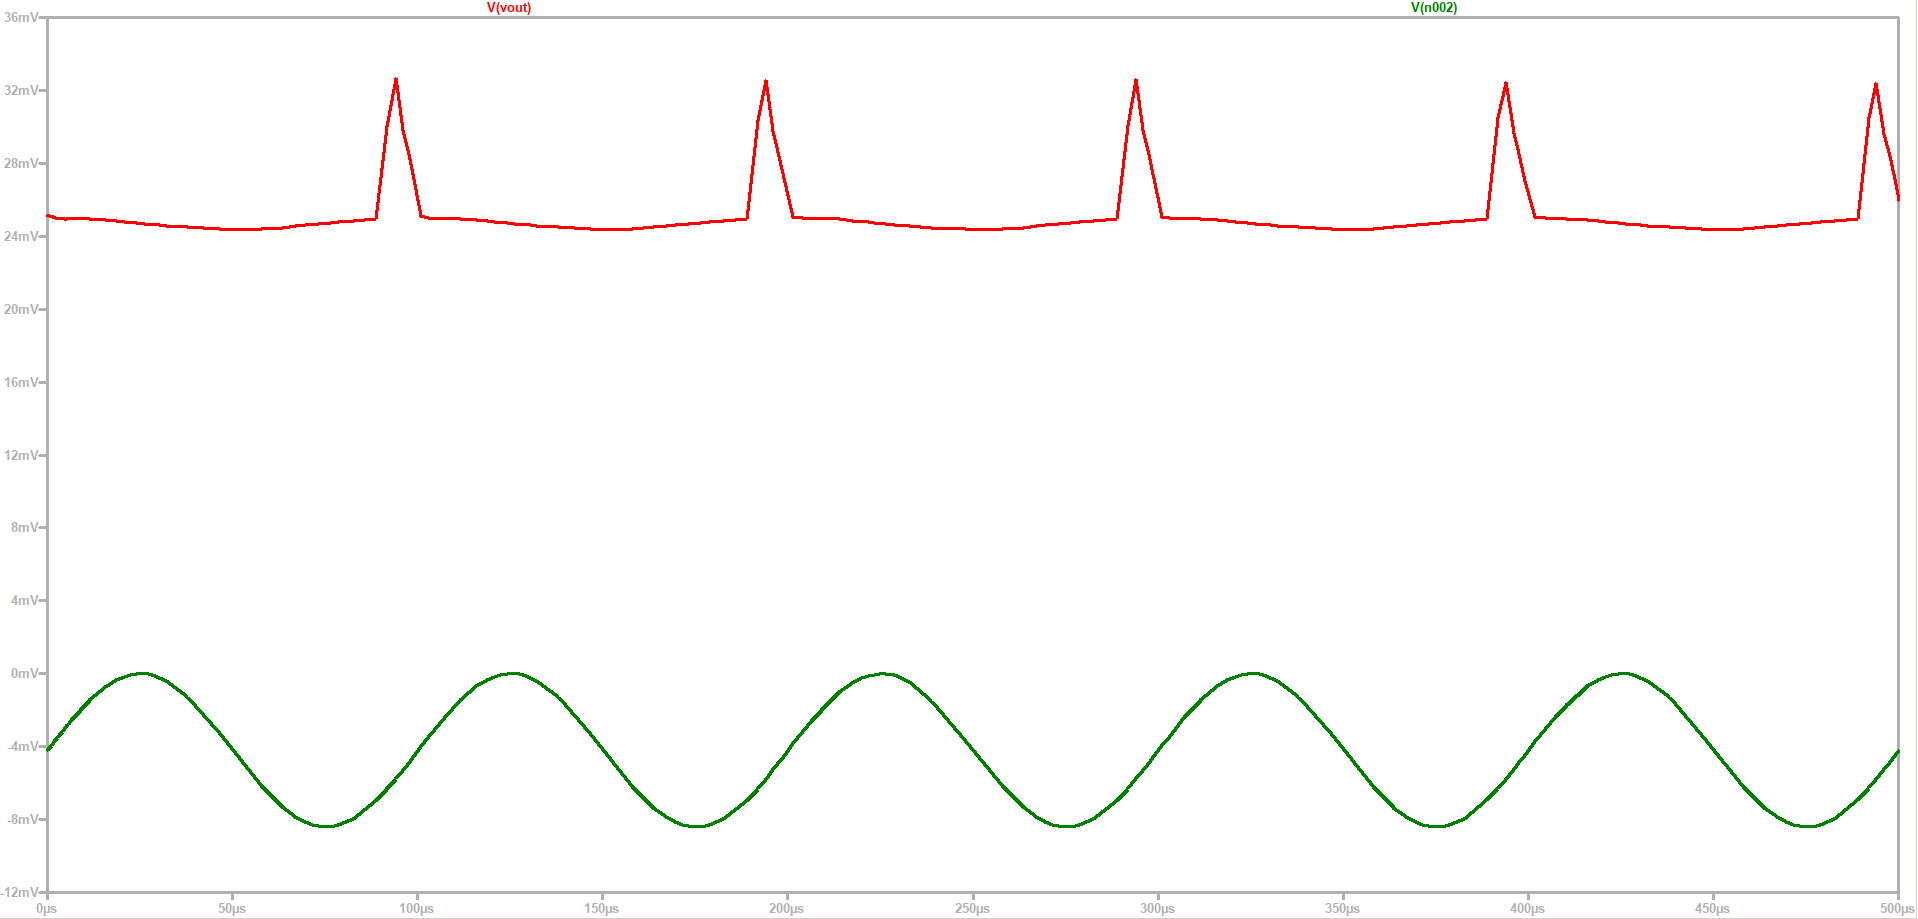
\includegraphics[width=0.7\linewidth]{Figures/Methodology/sig-cond-vsc-sine-sim-output-0042Vpp}
		\caption{Simulation results indicate that the \acrshort{vsc} circuit has a linear sensitivity of $\SI{70}{\micro\volt}$, compared to the linear sensitivity of $\SI{0.1}{\volt}$ in the vertical output of the HP8552B.}
		\label{fig:sig-cond-vsc-sine-sim-output-0024Vpp}
	\end{figure}  

	The above simulation results show that at $\SI{10}{\kilo\hertz}$, the \acrshort{vsc} circuit significantly distorts the shape of the vertical output from the HP8552B \acrshort{if} section for voltages near $\SI{0}{\volt}$. However, the performance of the circuit increases as the frequency increases. For example, no distortion or voltage clipping is evident for a sinusoidal input with a minimum value of $-\SI{0.32}{\volt}$ when the vertical output from the HP8552B has a frequency of $\SI{100}{\kilo\hertz}$, as illustrated by figure \ref{fig:sig-cond-vsc-sine-sim-output-100khz}.
	
	\begin{figure}[h!]
		\centering
		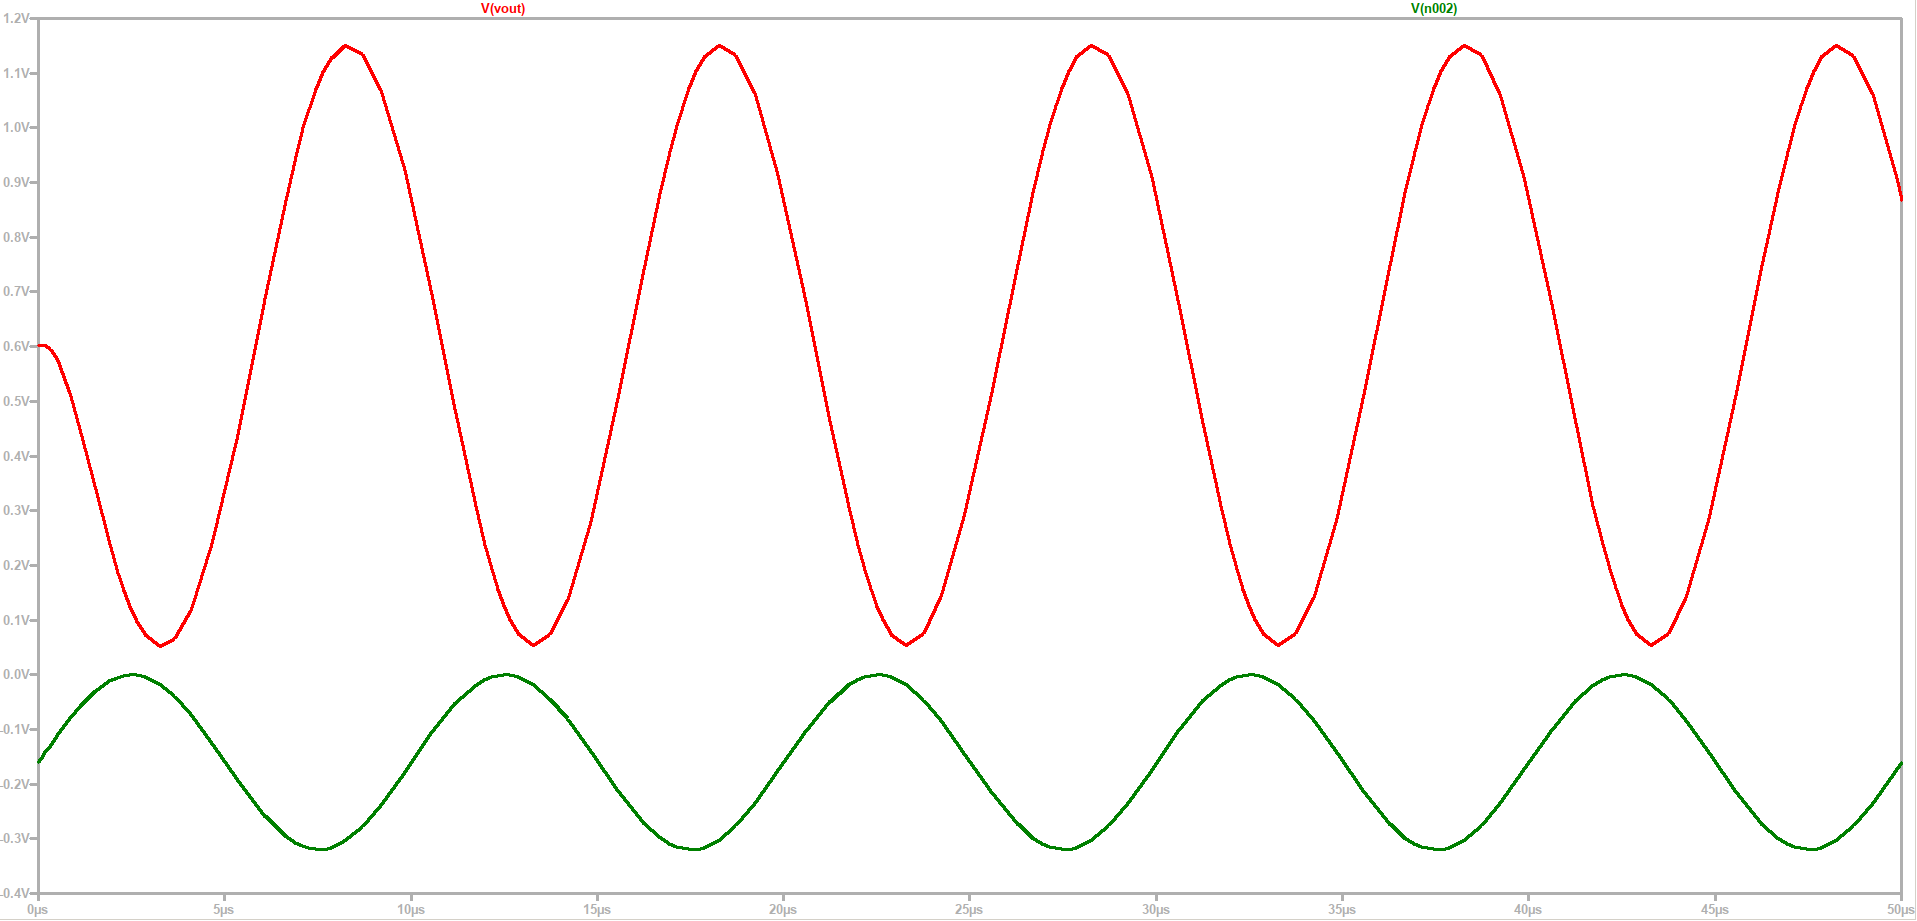
\includegraphics[width=0.7\linewidth]{Figures/Methodology/sig-cond-vsc-sine-sim-output-100khz}
		\caption{Showing reduced distortion and voltage clipping in the output for a vertical output frequency of $\SI{100}{\kilo\hertz}$.}
		\label{fig:sig-cond-vsc-sine-sim-output-100khz}
	\end{figure}  

	At $\SI{300}{\kilo\hertz}$, which is the expected maximum frequency in the vertical output of the \acrshort{if} section, the shape of the output is not affected, however, the phase difference between the input and the output is affected as seen in figure \ref{fig:sig-cond-vsc-sine-sim-output-300khz}. In addition, an offset of $\SI{37.27}{\milli\volt}$ is introduced at to the output of the \acrshort{vsc} circuit at higher frequencies of $\texttt{V}_\texttt{vin}$. 
	
	\begin{figure}[h!]
		\centering
		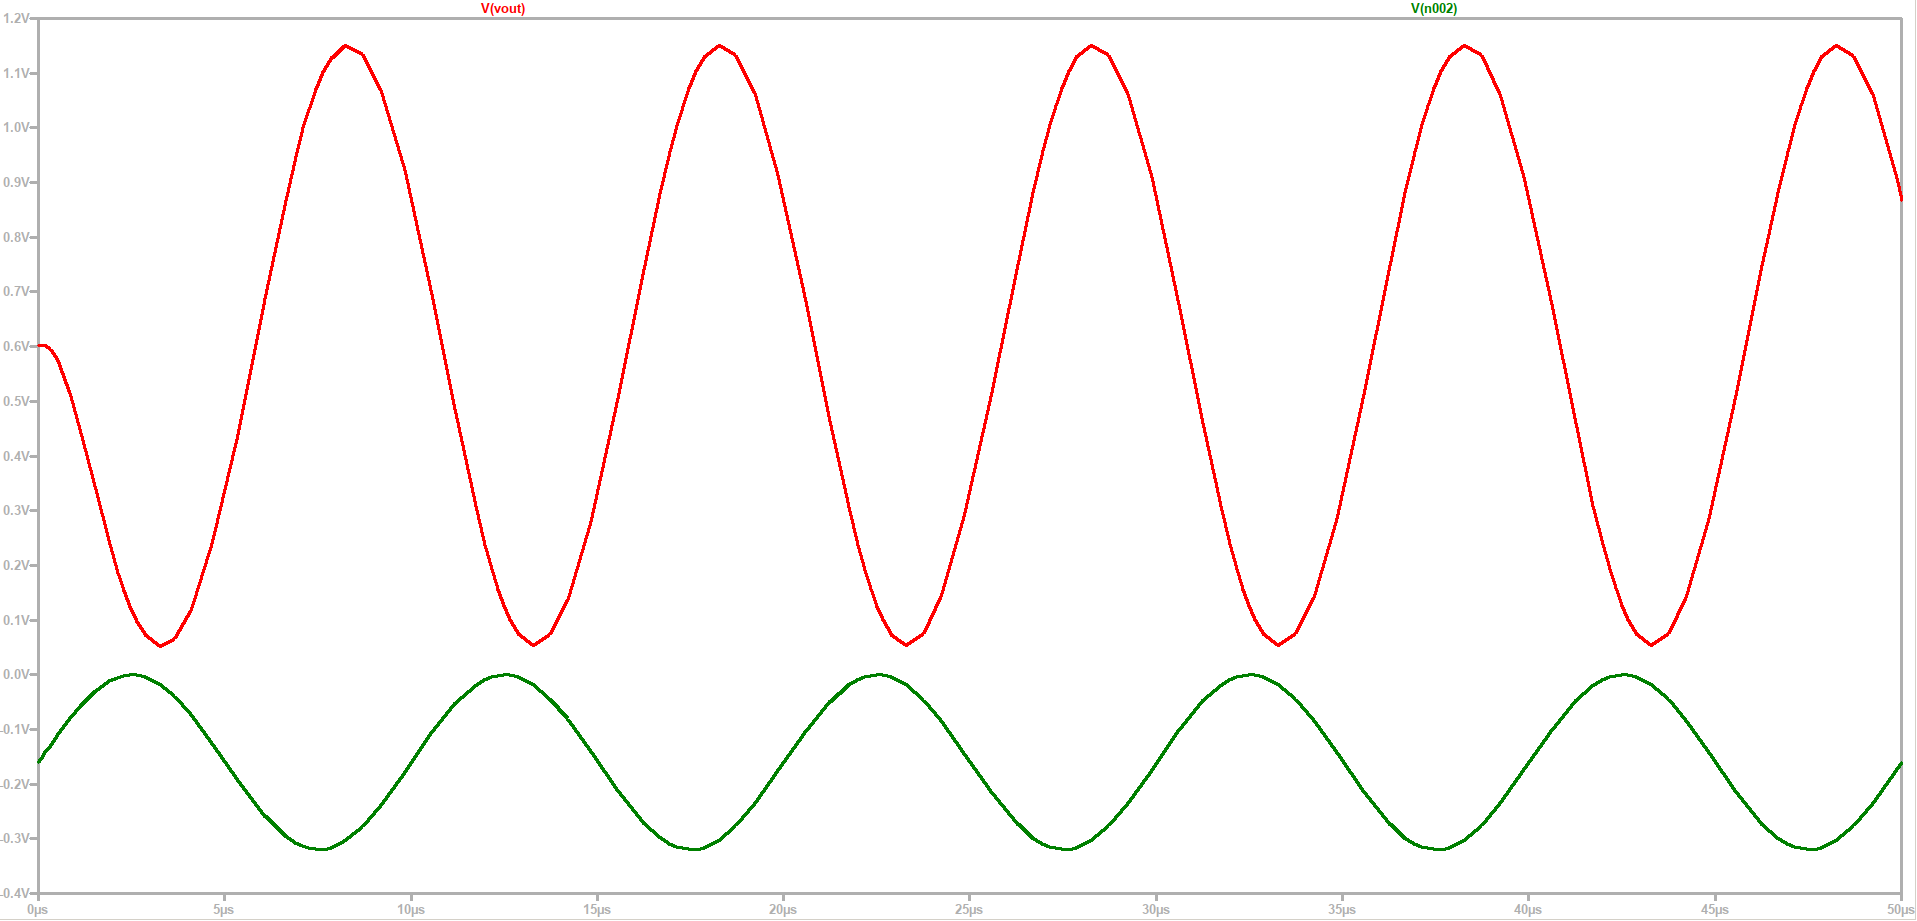
\includegraphics[width=0.7\linewidth]{Figures/Methodology/sig-cond-vsc-sine-sim-output-100khz}
		\caption{At the maximum rated vertical output frequency of $\SI{300}{\kilo\hertz}$, the phase difference between the input and the output of the \acrshort{vsc} is slightly more than $\pi\si{\radian}$.}
		\label{fig:sig-cond-vsc-sine-sim-output-300khz}
	\end{figure}  

	The specification of the \acrshort{scs} with respect to the \acrshort{vsc} pipeline are summarized in table \ref{tab:sig-cond-vsc-specs}.
	
	\begin{table}[ht!]
		\centering
		\label{tab:sig-cond-vsc-specs}
		\caption{Input and output specifications of the \acrshort{vsc}.}
		\begin{tabular}{ccc}
			
		\end{tabular}
	\end{table}
	
	The circuit for the \acrlong{plsc} pipeline is illustrated in figure \ref{fig:sig-cond-plsc-schematic} where an LM358 op-amp is used in the non-inverting buffer configuration which serves to scale the pen-lift output, $\texttt{V}_\texttt{penin}$, from the HP8552B plug-in of the HP141T system. 
	
	\begin{figure}[h!]
		\centering
		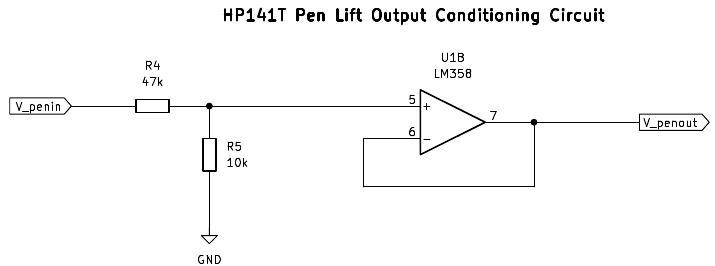
\includegraphics[width=0.7\linewidth]{Figures/Methodology/sig-cond-plsc-schematic}
		\caption{Schematic of the \acrshort{plsc} circuit for preparing the HP8552B pen-lift output for digital processing.}
		\label{fig:sig-cond-plsc-schematic}
	\end{figure}  
	
	The expected input voltage range of the \acrshort{plsc} circuit is $\SI{0}{\volt}$ to $\SI{14}{\volt}$, however, a LTSpice simulation of the circuit indicates that the maximum allowed value of $\texttt{V}_\texttt{penin}$ is $\SI{18.77}{\volt}$, corresponding to an output voltage of $\SI{3.3}{\volt}$. Simulation results are shown in figure \ref{fig:sig-cond-plsc-sim-output-1877V}, in which a pulse function was used to represent the \texttt{pen-up} ($\SI{18.77}{\volt}$) and \texttt{pen-down} ($\SI{0}{\volt}$) states. 
	
	\begin{figure}[h!]
		\centering
		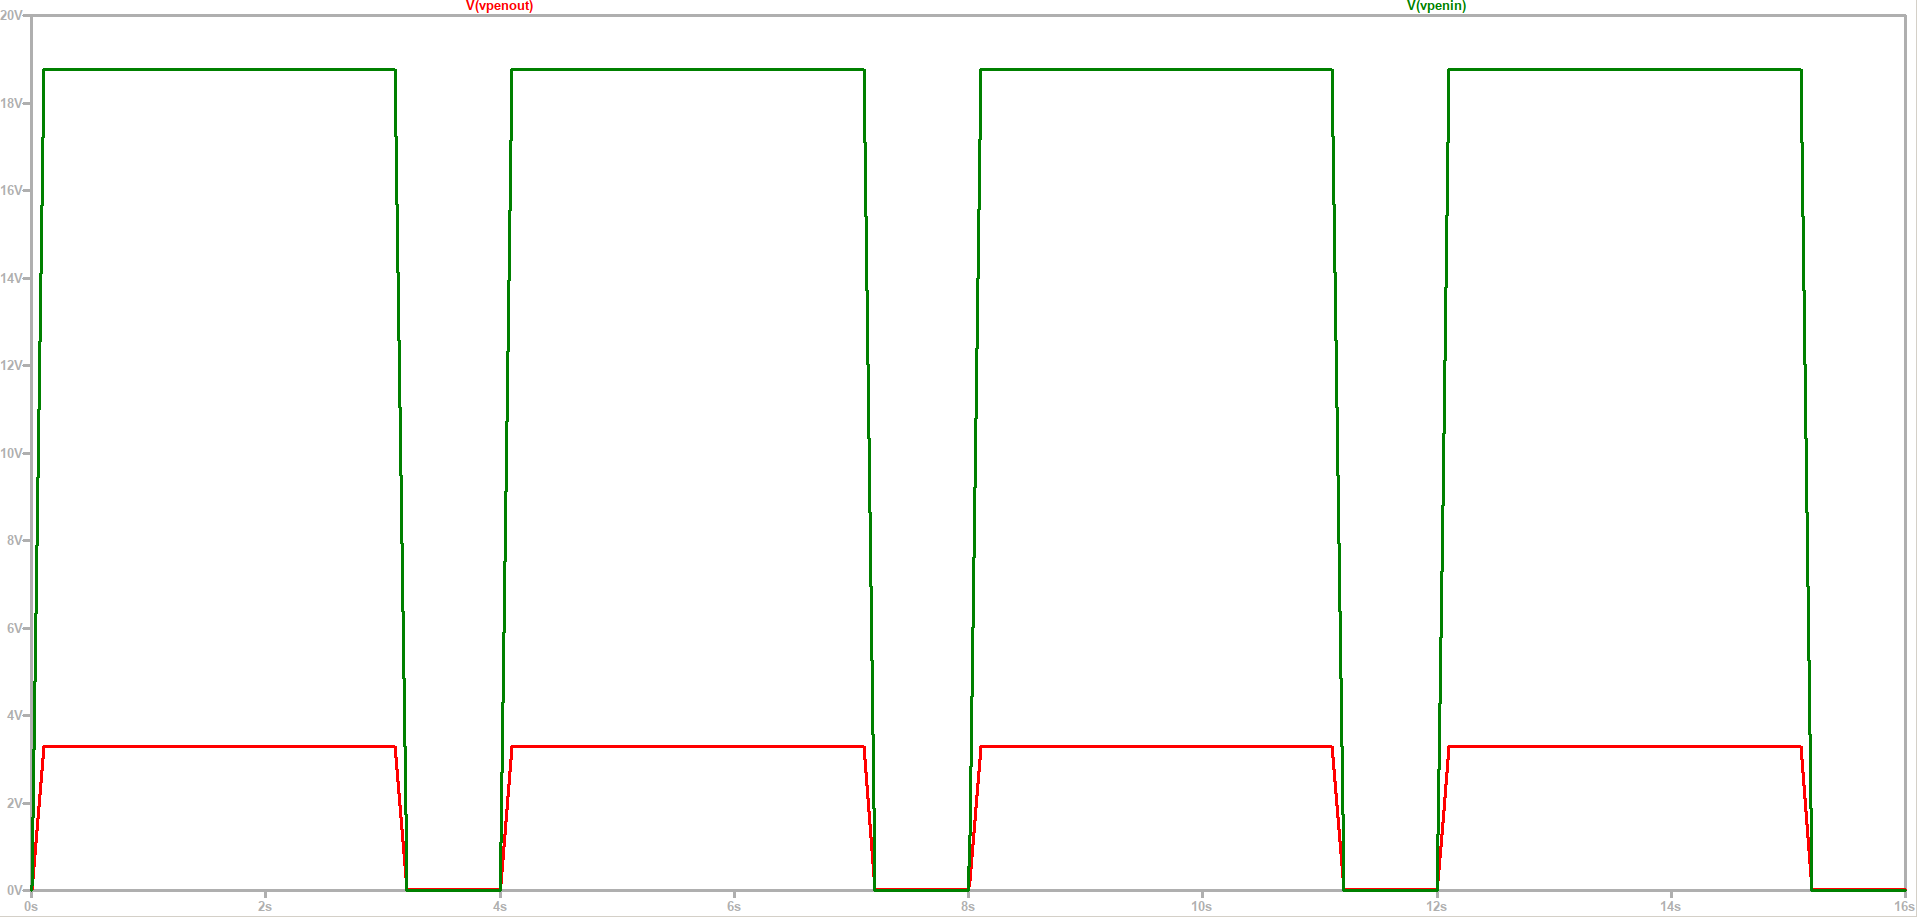
\includegraphics[width=0.7\linewidth]{Figures/Methodology/sig-cond-plsc-sim-output-1877V}
		\caption{Simulation result corresponding to the maximum operation voltage of the \acrshort{plsc} circuit corresponding to $\SI{18.77}{\volt}$.}
		\label{fig:sig-cond-plsc-sim-output-1877V}
	\end{figure}

	A full 3D model of the \acrshort{scs} \acrshort{pcb} is depicted in figure \ref{fig:scs-pcb} which uses the 8-pin chip with 2 LM358s in on packaging. Since 3 op-amps are used in the \acrshort{scs}, a total of 2 chips is required for the full implementation of the subsystem. Op-amps are powered by a $\SI{9}{\volt}$ battery as illustrated in figure \ref{fig:scs-power-schematic}. Connection to the power source is controlled using a 3-pole switch. When the switch is ON, the power \acrshort{led} is active and when the switch is OFF, no power is supplied to the \acrshort{pcb} and the \acrshort{led} is inactive. 

	\begin{figure}[ht!]
		\centering
		\begin{subfigure}{.5\textwidth}
			\centering
			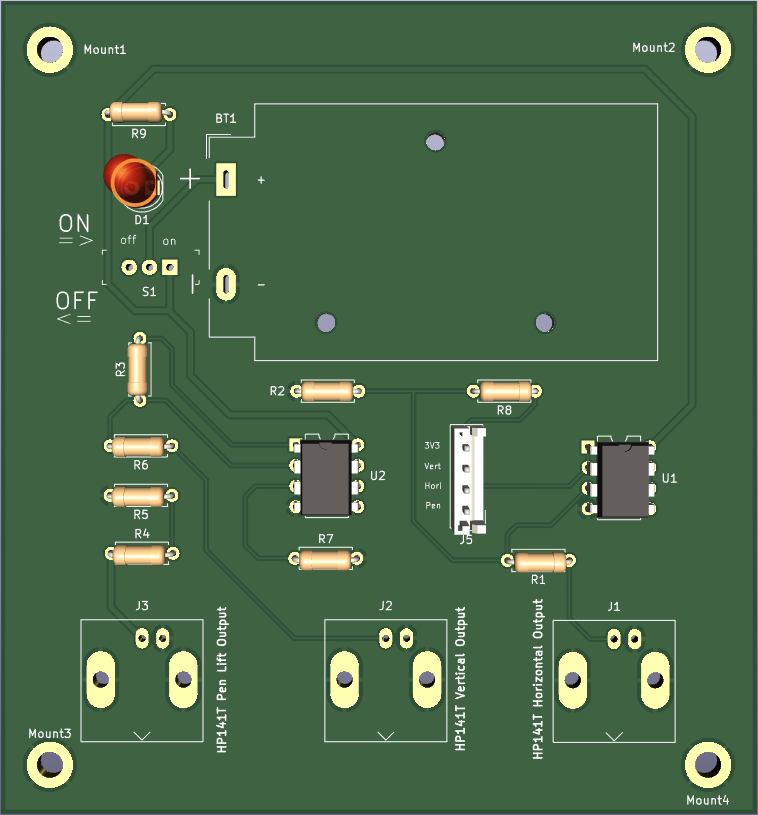
\includegraphics[width=0.7\linewidth]{Figures/Methodology/scs-pcb}
			\caption{A 3D model of the \acrshort{scs} \acrshort{pcb}.}
			\label{fig:scs-pcb}
		\end{subfigure}%
		\begin{subfigure}{.5\textwidth}
			\centering
			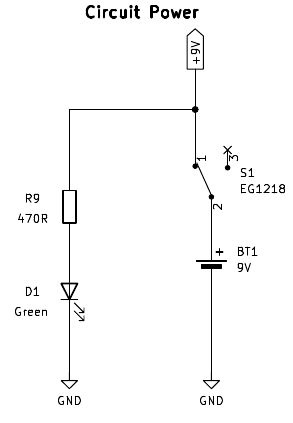
\includegraphics[width=0.57\linewidth]{Figures/Methodology/scs-power-schematic}
			\caption{Schematic of the \acrshort{scs} power supply circuit.}
			\label{fig:scs-power-schematic}
		\end{subfigure}
		\caption{The \acrshort{scs} is implemented on a single \acrshort{pcb} with a single $\SI{9}{\volt}$ power source.}
		\label{fig:scs-full-subsystem}
	\end{figure}

	The physical hardware specifications of the \acrshort{vsc} \acrshort{pcb} are shown in figure \ref{tab:sig-cond-vsc-hardware-specs}. The \acrshort{pcb} was designed using KiCad 6 to consist of a porous GND copper layer for establishing a reference voltage for the through-hole components. Surface mount holes are also grounded to prevent electric shock and ensure safety. 
	
	\begin{table}[ht!]
		\centering
		\label{tab:sig-cond-vsc-hardware-specs}
		\caption{Input and output specifications of the \acrshort{vsc}.}
		\begin{tabular}{ccc}
			
		\end{tabular}
	\end{table}

	\subsubsection{Data Acquisition Subsystem}
	
	The \acrfull{das} is responsible for converting conditioned analog signals from the \acrshort{scs} into digital values for further processing. Therefore, the \acrshort{das} forms a critical part of the digitization of the HP141T system. It enables subsequent manipulation by the \acrlong{dps} and \acrshort{guis}. The \acrshort{das} ensures that the output analog signals from the \acrshort{scs}, i.e. $\texttt{V}_\texttt{hout}$, $\texttt{V}_\texttt{vout}$ and $\texttt{V}_\texttt{penout}$, which are the scaled and shifted versions of the outputs from the HP8552B plug-in, are accurately sampled and converted into digital values suitable for processing by a \acrshort{mcu} and \acrshort{sbc}. 
	
	The diagram in figure \ref{fig:das-subsystem-diagram} illustrates the functionality of the \acrshort{das} where an \acrshort{adc} samples the analog inputs at a rate sufficient for capturing high frequency components (up to $\SI{300}{\kilo\hertz}$ for the vertical channel). The digitized output values of the \acrshort{das} represent the amplitude and timing of the signals which is crucial for reconstructing the frequency spectrum of the input signal at the input of the HP8555A \acrshort{rf} section.
	
	\begin{figure}[h!]
		\centering
		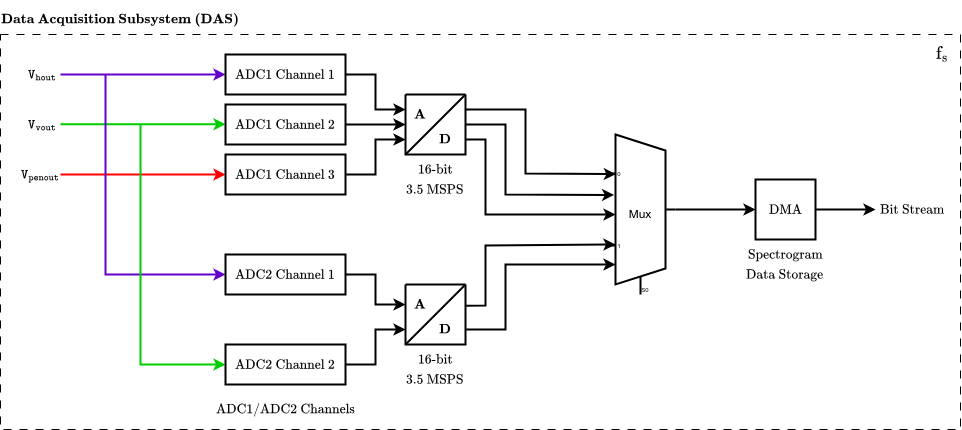
\includegraphics[width=0.7\linewidth]{Figures/Methodology/das-subsystem-diagram}
		\caption{\acrshort{das} subsystem block diagram showing the digitization of the analog signals using 2 16-bit \acrshort{adc}s operating in double-interleaved mode.}
		\label{fig:das-subsystem-diagram}
	\end{figure} 
	
	The \acrshort{das} uses the two 16-bit resolution \acrshort{adc}s in double-interleaved mode. Given that the outputs of the \acrshort{scs} assume values up to a reference voltage of $\SI{3.3}{\volt}$, the \acrshort{das} can represent 65565 values in $\SI{50.35}{\micro\volt}$ intervals. In 16-bit mode, the sampling rate of each \acrshort{adc} can reach up to $3.5$ \acrshort{msps} which implies that the system throughput can reach a total $7$ \acrshort{msps} when the \acrshort{adc}s are configured in dual fast interleaved mode as illustrated in figure \ref{fig:das-adc-df-interleaved-mode}. 
	
	\begin{figure}[h!]
		\centering
		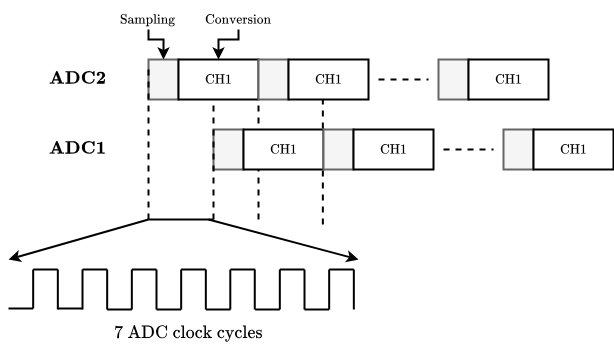
\includegraphics[width=0.55\linewidth]{Figures/Methodology/das-adc-df-interleaved-mode}
		\caption{ADC1 and ADC2 convert the voltages in a period of 7 \acrshort{adc} clock cycles on the same channel.}
		\label{fig:das-adc-df-interleaved-mode}
	\end{figure} 
	
	In dual mode, ADC1 is the master and ADC2 is the slave. The pen-lift signal from the \acrshort{scs} behaves like a trigger which is internally synchronised for channel conversion. In dual fast interleaved mode, each \acrshort{adc} converts the channel every 14 \acrshort{adc} clock cycles and are stored into the ADC1 data register in a 32-bit format \cite{stm32adcmodes}. The Nyquist criteria requires that the sampling frequency rate should be higher than or equal to twice the frequency of the signal to be converted. Since the maximum frequency of the signals from the \acrshort{scs} circuit is $\SI{300}{\kilo\hertz}$, a $3.5$ \acrshort{msps} rate meets the $600$ kSPS needed for the vertical output. To ensure high integrity in data transfer, the \acrfull{das} subsystem uses DMA2 for the master \acrshort{adc} and DMA1 for the slave. 
	
	Results from a MATLAB simulation of the dual interleaved \acrshort{adc} operation are shown in figure \ref{fig:das-matlab-sim} where ADC1 and ADC2 alternate samples to double the sampling rate in order to satisfy the required 801 data points. The simulation calculates a \acrshort{snr} of $\SI{78}{\decibel}$ with $\SI{1}{\milli\volt}$ Gaussian noise. A table of summarizing the specifications modelled in the simulation is shown in \ref{tab:das-matlab-sim-specs}.
	
	\begin{table}[ht!]
		\centering
		\label{tab:das-matlab-sim-specs}
		\caption{Specifications of the \acrshort{das}.}
		\begin{tabular}{ccc}
			
		\end{tabular}
	\end{table}
	
	\begin{figure}[h!]
		\centering
		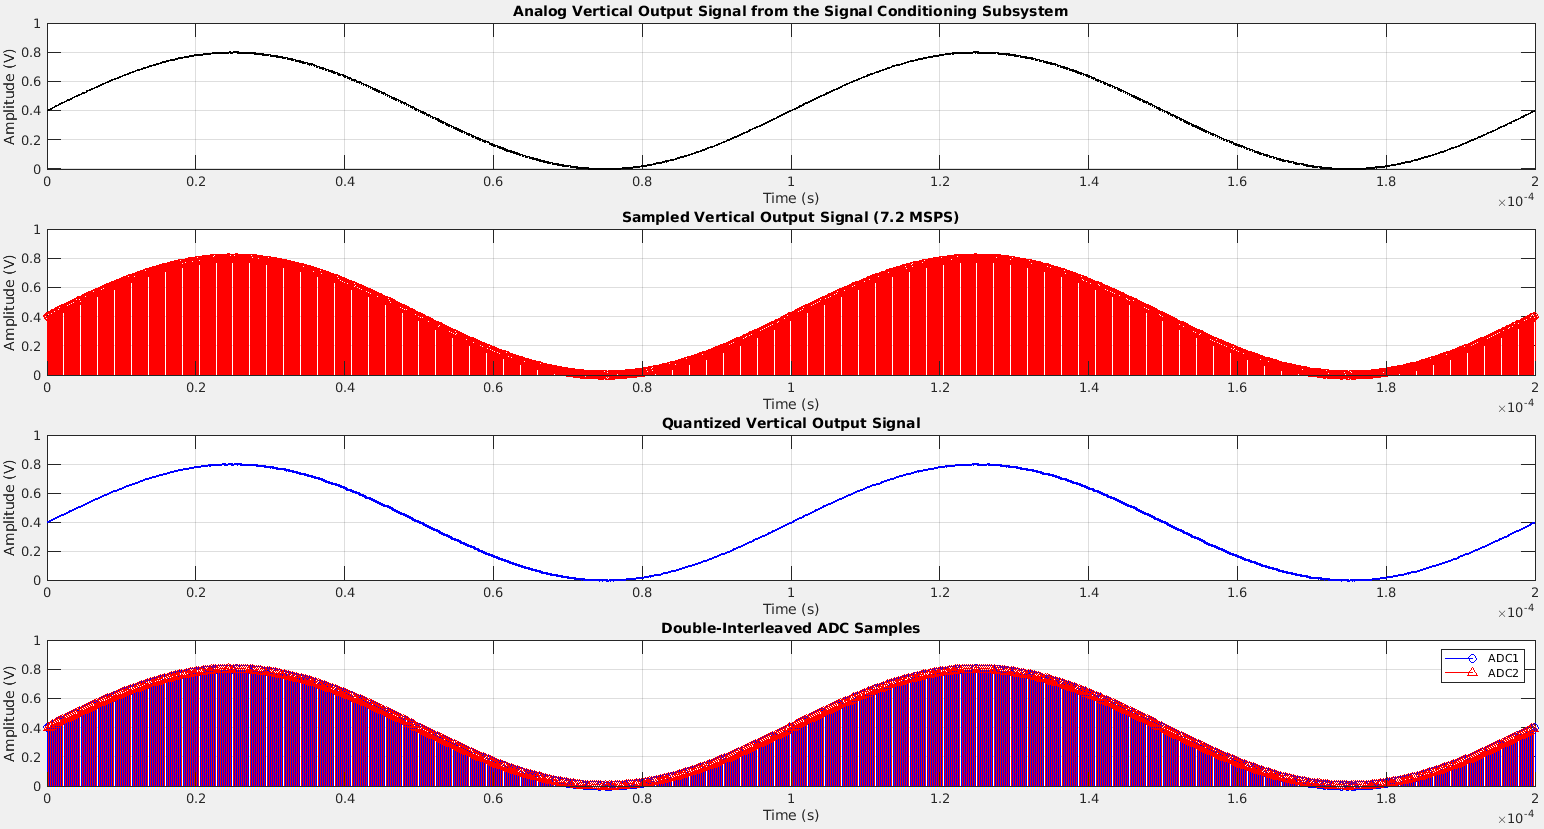
\includegraphics[width=0.70\linewidth]{Figures/Methodology/das-adc-sim}
		\caption{Simulation results of a well-behaved sinusoidal signal that is sampled by the \acrshort{adc}s on the STM32H723ZG development board.}
		\label{fig:das-matlab-sim}
	\end{figure} 
	
	Figure \ref{fig:das-matlab-sim} shows the results from running the simulation with a well-behaved, sinusoidal analog vertical output signal from the \acrshort{scs} with a frequency of $\SI{10}{\kilo\hertz}$ and a conditioned peak-to-peak voltage of $\SI{0.8}{\volt}$. Given that the \acrshort{adc}s are operating with a 16-bit resolution, the subsequently high number of quantized levels allow for a smooth sample with closely spaced data points as seen in the second and third plots in the figure. The final figure illustrates the output of the \acrshort{adc}s operating in double-interleaved mode. Samples from the master \acrshort{adc} are shown in red while samples from the slave are shown in blue. 
	
	Results from a more accurate simulation are shown in figure \ref{fig:das-adc-sim-noisy} where the \acrshort{scs} outputs a noisy signal as input to the \acrshort{das}. The results illustrate that as long as the voltage is within the range $\SI{3.3}{\volt}$, the double interleaved mode is able to capture the a large number of samples to closely represent the input signal. The \acrshort{das} propagates errors from the \acrshort{scs} circuit which prepares the analog outputs from the HP8552B. 
	
	\begin{figure}[h!]
		\centering
		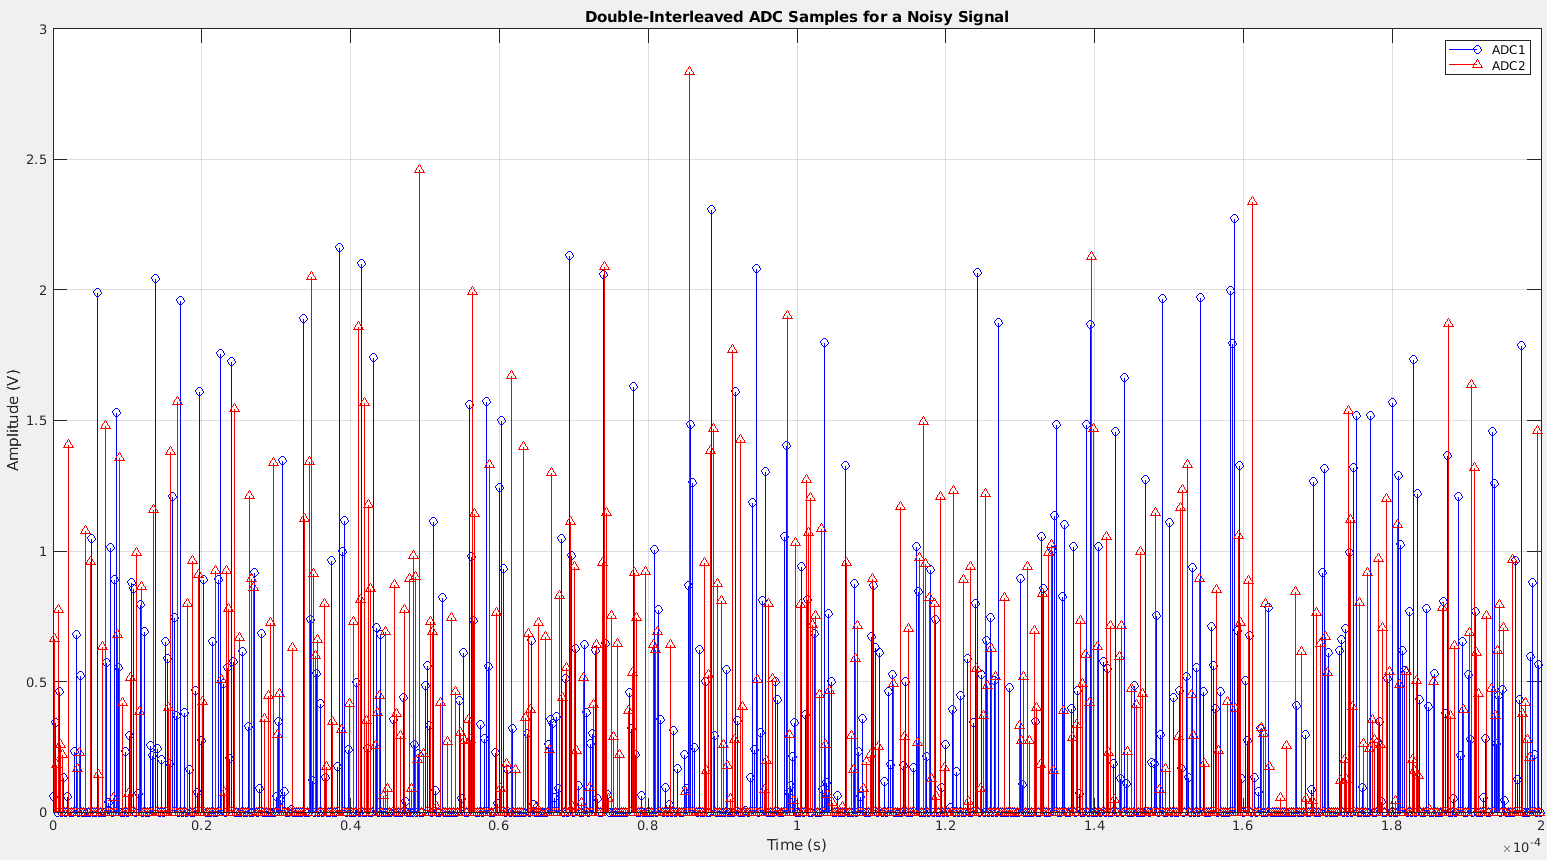
\includegraphics[width=0.70\linewidth]{Figures/Methodology/das-adc-sim-noisy}
		\caption{Simulation of a noisy signal sampled in double-interleaved mode by ADC1 and ADC2 on the STM32H723ZG.}
		\label{fig:das-adc-sim-noisy}
	\end{figure} 

	The behaviour of the \acrshort{das} is implemented on the STM32H723ZG \acrshort{mcu} using embedded C to sample signals using functions in the \acrfull{hal} library. The horizontal ($\texttt{V}_\texttt{x}$), vertical ($\texttt{V}_\texttt{y}$) and pen-lift ($\texttt{V}_\texttt{z}$) outputs are mapped to PF10 (\texttt{ADC1\_PIN8}), PF9 \texttt{ADC1\_PIN7} and PF8 \texttt{ADC1\_PIN6}, respectively. The code snippet in listing \ref{lst:das-adc-macros} in the appendices shows the definition of the macros including the \texttt{DMA\_REQUEST\_ADC1} macro which enables the system to stream data to a buffer using \acrshort{dma}. The \texttt{DMA2\_Stream0\_IRQHandler} macro handles \acrshort{dma} interrupts for the \acrshort{adc} data streaming by calling the \acrshort{hal} \acrshort{dma} handler to process events such as a full buffer. The \acrshort{das} uses a \texttt{uint16\_t} buffer size of 802, corresponding to 401 samples per \acrshort{adc} channel. 
	
	The STM32H723ZG shares the same clock for the master and slave \acrshort{adc}s, derived from the peripheral clock PLCK2 to be divided by a factors of 2. The proposed design derives the \acrshort{adc}s' clock via a \acrshort{adc} prescaler (\texttt{ADC\_CLOCKPRESCALER\_PCLK\_DIV4}) of 4 and a APB2 prescaler of 2, to achieve a sample achieve a frequency of $\SI{36}{\mega\hertz}$. The sampling rate depends on the \acrshort{adc} clock frequency $F_{ADC}$, sampling period $T_{ADC}$, and conversion time $T_{CONV}$. At $\SI{36}{\mega\hertz}$ and a total of 19 cycles per sample, a single \acrshort{adc}'s sampling period is $\SI{0.528}{\micro\second}$ per sample (or 1.89 \acrshort{msps}). The full sampling capability of the \acrshort{adc}s can be achieved by setting the \acrshort{adc} clock to $\SI{60}{\mega\hertz}$ and using 18 cycles per second, giving a sample rate of 6.66 \acrshort{msps}. The \texttt{adc\_error\_flag} global variable is initialized to zero and is used to track \acrshort{adc} initialization errors for debugging. 
	
	The \texttt{HAL\_DMA\_IRQHandler} function from the STM32H7 \acrshort{hal} \acrshort{api} is used to handle \acrshort{dma} interrupts for the master \acrshort{adc} and triggers callbacks. Given that only the master's \acrshort{dma} handles all data transfers, no \acrshort{dma} is required for the slave \acrshort{adc}. Processed \acrshort{adc} data is stored using the \texttt{spectrogram\_t} structure which is initialized as a pointer as shown in listing \ref{lst:das-spectrogram-init-code}. 
	
	\begin{lstlisting}[language=C, label={lst:das-spectrogram-init-code}, caption={The \texttt{HAL\_DMA\_IRQHandler} function is used to handle \acrshort{dma} transfers while the \texttt{adc\_set\_spectrogram(spectrogram\_t *s)} function is used to initialize a pointer to a \texttt{spectrogram} structure.}]
	void adc_error_handler(void) {
		adc_error_flag = 1;
		while(1) {}
	}
	
	spectrogram_t *adc_spectrogram = 0;
	
	void adc_set_spectrogram(spectrogram_t *s) {
		adc_spectrogram = s;
	}
	\end{lstlisting}
	
	The \texttt{adc\_init} function forms a critical part of the \acrshort{das} because it initializes ADC1 as the master and ADC2 as the slave in double-interleaved mode, configures three sampling channels, and begins \acrshort{dma} transfers as shown in listing \ref{lst:das-spectrogram-init-code} in Appendix A. In addition, the function sets the resolution to 16-bits and enables a continuous mode for uninterrupted conversions for seamless real-time data acquisition. The development board is configured by the \texttt{ADC\_DUALMODEDATAFORMAT\_32\_10\_BITS} variable to use outputs with 32-bit words, however, the \texttt{adc\_buffer} is \texttt{uint16\_t}. Therefore, the \acrshort{hal} is expected to extract the lower 16 bits. 
	
	\acrshort{adc} data that is stored in the \texttt{adc\_spectrogram} structure is processed using conversion callbacks such as the \texttt{HAL\_ADC\_ConvHalfCpltCallback} in listing \ref{lst:das-callbacks} used when the \acrshort{dma} is half-full. The function reads interleaved data, corresponding to values of $\texttt{V}_\texttt{x}$, $\texttt{V}_\texttt{y}$ and $\texttt{V}_\texttt{z}$ from the \texttt{adc\_buffer}. Three variables, \texttt{x}\_\texttt{val}, \texttt{y}\_\texttt{val} and \texttt{z}\_\texttt{val} are scaled and inverted according to the 16-bit resolution of the \acrshort{adc}s. For example, \texttt{x}\_\texttt{val} is scaled to \texttt{npoints} by dividing by 65536, corresponding to a 16-bit scaling which matches the resolution of the \acrshort{adc}s. The pen-lift output, $\texttt{V}_\texttt{z}$, is assigned a threshold value of 32768, corresponding to $\SI{1.2}{\volt}$ for the \texttt{pen-down} state as shown in the simulation results. The threshold value is expected to require adjustments if the \acrshort{scs} output is slightly higher or lower than the simulated outputs. 
	\begin{lstlisting}[language=C, label={lst:das-callbacks}, caption={Showing conversion callbacks for processing \acrshort{adc} data when the \acrshort{dma} fills half.}]
	void HAL_ADC_ConvHalfCpltCallback(ADC_HandleTypeDef* AdcHandle) {
		for (int j = 0; j < ADC_BUF_SIZE/6; ++j) {
			uint32_t x_val = adc_buffer[j*3];     // V_x
			uint32_t y_val = adc_buffer[j*3+1];   // V_y
			uint32_t z_val = adc_buffer[j*3+2];   // V_z
			x_val = (x_val * adc_spectrogram->npoints) / 65536; // 16-bit scaling
			y_val = adc_spectrogram->size_y - (adc_spectrogram->size_y * y_val) / 65536;
			z_val = z_val > 32768 ? 1 : 0; // Threshold at mid-scale (~1.65 V)
			if (x_val < 5) prev_x = 0;
			if (x_val > prev_x && z_val == 0) {
				if (pending_normalization) {
					adc_spectrogram->data_normal[x_val] = adc_spectrogram->size_y/2 - y_val;
				}
				adc_spectrogram->data[x_val] = y_val + adc_spectrogram->data_normal[x_val];
				prev_x = x_val;
			}
		}
	}
	\end{lstlisting}
	The code design implements the \texttt{HAL\_MspInit} callback function, shown in listing \ref{lst:das-callbacks} to perform system level initializations as indicated in the \acrshort{hal} manual for the STM32H7 series. This function enables clocks for the \acrshort{adc}s, GPIOF, and DMA2, in addition to configuring the correct pins as analog inputs. Clocks and \acrshort{gpio} pins are enable with analog mode and no pull up resistors. 
	\begin{lstlisting}[language=C, label={lst:das-callbacks}, caption={Showing conversion callbacks for processing \acrshort{adc} data when the \acrshort{dma} fills half.}]
		void HAL_ADC_MspInit(ADC_HandleTypeDef *hadc) {
			GPIO_InitTypeDef GPIO_InitStruct = {0};
			static DMA_HandleTypeDef hdma_adc;
			
			if (hadc->Instance == ADCx_MASTER) {
				/* Enable clocks */
				ADCx_CLK_ENABLE();0
				ADCx_CHANNEL_GPIO_CLK_ENABLE();
				DMAx_CLK_ENABLE();
				//...
				/* Configure GPIO pins */
				GPIO_InitStruct.Pin = ADCx_CHANNEL_PIN | ADCx_CHANNEL_PIN2 | ADCx_CHANNEL_PIN3;
				GPIO_InitStruct.Mode = GPIO_MODE_ANALOG;
				GPIO_InitStruct.Pull = GPIO_NOPULL;
				//...
				hdma_adc.Init.PeriphDataAlignment = DMA_PDATAALIGN_HALFWORD; // 16-bit
				hdma_adc.Init.MemDataAlignment = DMA_MDATAALIGN_HALFWORD;
				hdma_adc.Init.Mode = DMA_CIRCULAR;
				//...
				__HAL_LINKDMA(hadc, DMA_Handle, hdma_adc);
				
				/* Configure NVIC */
				HAL_NVIC_SetPriority(ADCx_DMA_IRQn, 0, 0);
				HAL_NVIC_EnableIRQ(ADCx_DMA_IRQn);
			}
	\end{lstlisting}
	Note that the \acrshort{dma} is used is circular mode to support continuous data acquisition. The \texttt{DMA\_PDATAALIGN\_HALFWORD} variable aligns with 16-bit data corresponding to half a 32-bit word. Furthermore, the board is designed to use and \acrfull{nvic} as a higher-priority interrupt for ensuring timely \acrshort{dma} handling for real-time data acquisition. 
	
	Due to time constraints and low availability of the STM32H723ZG development board, the device includes the output spectrogram of the \acrshort{das} is stored in the \texttt{.csv} format with 4 columns for the time-stamp ($\si{\milli\second}$) and the interleaved data samples corresponding to $\texttt{V}_\texttt{x}$, $\texttt{V}_\texttt{y}$, and $\texttt{V}_\texttt{z}$ (in $\si{\volt}$). 
	
	HP141T system samples stored in the \texttt{.csv} file differ from HP141T Emulator samples based on the simulation results. For example, the simulated output at the STO pin of the XR2206 chip in the vertical output emulator circuit is expected to range between $\SI{0}{\volt}$ to $\SI{3.0}{\volt}$ instead of the $\SI{0}{\volt}$ to $\SI{3.3}{\volt}$ range output from the \acrshort{scs} circuit for inverting the original output from the HP141T. Note that although the sampled data is used to construct a spectrogram in the frequency domain, the actual values are interpreted in the time domain - directly associated with data points in the amplitude vs frequency plots representing the frequency domain characteristics of the inputs signal. 
	
	A Picoscope 2204A \acrshort{usb} oscilloscope was selected as an alternative device for sampling because of its ability to acquire data at a maximum sampling rate of $100$ \acrshort{msps}, which would sufficiently satisfy requirements UR01 and SR01. The Picoscope 2204A is the smallest oscilloscope in the 2000 Series, which includes a range of 8-bit oscilloscopes with sample rates of up to 1 \acrshort{gsps}. In addition, the hand-held oscilloscope can output data in a group of \texttt{.csv} files with two columns for the time-stamp and sampled voltage, separately for two channels. Both alternative sampling devices (STM32H7 and Picoscope) aim to satisfy the design requirement for enabling trace storage capabilities (UR06).
		
	Given that the Picoscope has two channels, $A$ and $B$ as shown in figure \ref{fig:das-picoscope}, data acquisition using the hand-held oscilloscope is performed continuously for the vertical and horizontal outputs. The pen-lift output can be analysed on an isolated channel during unit tests for ensuring that hardware subsystems are operating as expected. Alternatively, the vertical and pen-lift outputs can be used without the scan output by plotting interpolated samples of the vertical output. To sample data, the oscilloscope uses probes which can connect to connector pins on the HP141T Emulator and \acrshort{scs} circuits. 
	
	\begin{figure}[h!]
		\centering
		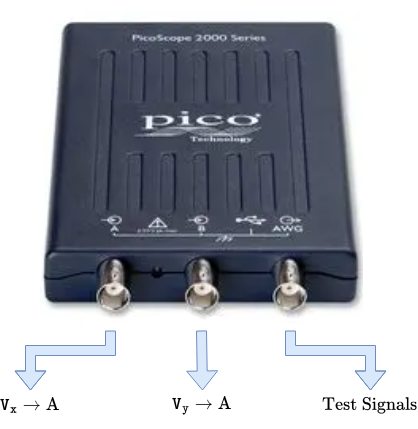
\includegraphics[width=0.37\linewidth]{Figures/Methodology/das-picoscope}
		\caption{Illustrating how the outputs of the HP141T can be sampled using input channels A and B on the Picoscope 2204A.}
		\label{fig:das-picoscope}
	\end{figure} 

	Picoscope samples can be visualized using the Picoscope 7 Software which includes multiple analysis tools such as visualizations of the amplitude vs frequency spectrum of the input. In addition to being a substitute sampling device for the STM32H723ZG board, the design employs the \acrshort{usb} oscilloscope and accompanying Picoscope 7 Software to verify the operation of the HP141T Emulator and \acrshort{scs} circuits. The Picoscope 7 visualization tool display is only used during testing to determine if hardware operates as expected - in line with the behaviour of the simulated circuits.
	
	\subsection{Digital Processing Subsystem}
	
	The aim of the \acrshort{dps} is to prepare the data for display in the \acrshort{guis} and fulfil the requirement for the digitized \acrshort{sa} to have 3 display modes associated with UR02. The subsystem uses Python to accomplish the tasks associated with each display mode. For example, the peak hold mode uses the \texttt{max()} function to find the maximum amplitude and corresponding frequency in the spectrogram data stored as an iterable object. Since spectrogram data can be retrieved from the STM32H7 \acrshort{adc} samples or from values sampled by the hand-held usb oscilloscope, construction of the spectrogram is considered as the first step in the flow of the \acrshort{das}, illustrated in figure \ref{fig:dps-pipeline} which demonstrates how the time domain signal is processed to display the frequency domain characteristics of an input to the HP8555A plug-in. Most of the data processing occurs on the Raspberry Pi 4B, which is proposed for handling digital processes and displays through a \acrshort{lcd} touch-screen in the \acrshort{guis}.
	
	\begin{figure}[ht!]
		\centering
		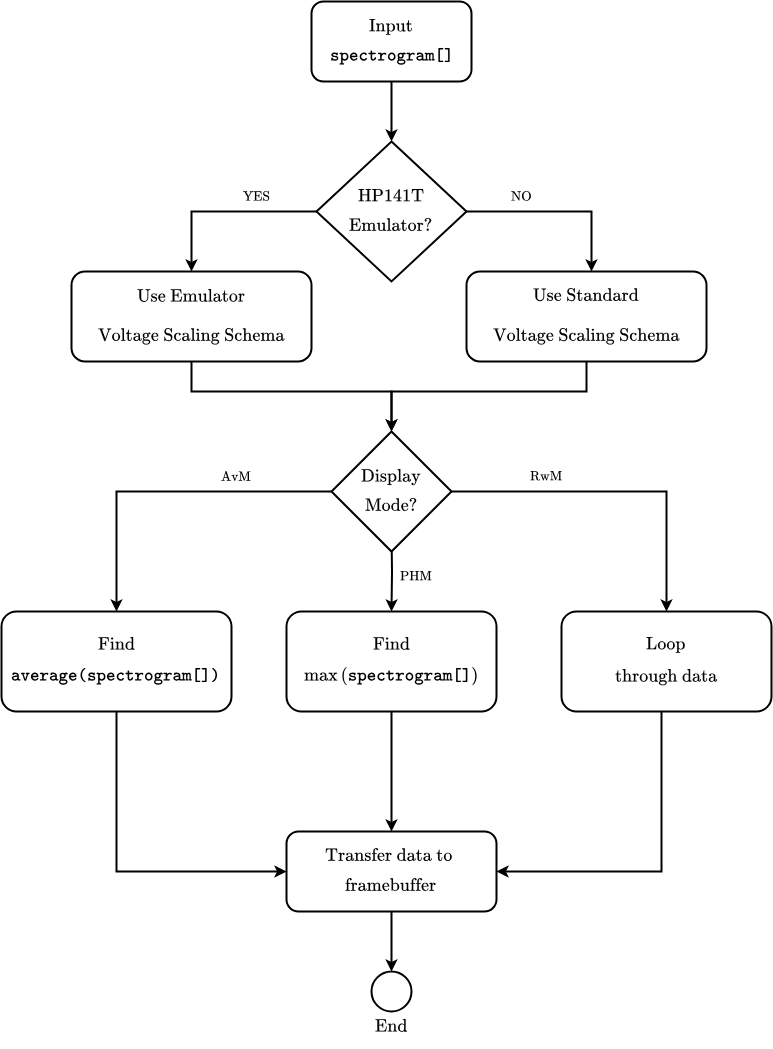
\includegraphics[width=0.58\linewidth]{Figures/Methodology/dps-pipeline}
		\caption{Flow diagram of the \acrlong{dps} which prepares time domain data for display in the frequency domain through the \acrlong{guis}.}
		\label{fig:dps-pipeline}
	\end{figure} 

	The flow diagram shows that the methods used for processing sampled data depends on the whether input data is from the standard data from the HP141T system or the HP141T Emulator for cases where access the \acrshort{sa} is limited. In other words, if the system being measured is the HP141T system with the original outputs, then the \acrfull{svsis} is used to convert the data to appropriate values for the \acrfull{hvs} which is later used by the \acrshort{guis} for drawing the plot on the touchscreen. If measurements of the HP141T Emulator are taken, then the \acrfull{evsis} is used to scale the time domain values in the iterable spectrogram data. In the subsequent steps, the \acrshort{dps} assesses the user-selected display mode to determine which operation to perform. Different functions, such as the \texttt{average\_spectrogram()} which updates the frequency bin's average at each scan. This subsection describes the scaling and interpolation algorithms, and the principle functions for each display mode used to process the data in the \acrshort{dps} for display in the \acrshort{guis}.
	
	To ensure that the \acrshort{das} can integrate seamlessly with the \acrfull{dps} and \acrfull{guis}, regardless of the sampling device that is available between the STM32H7 and Picoscope, the code for the spectrogram structure, adopted from a similar project designed to run on an STM32F746G Discovery board, was modified to process sampled data from 3 \acrshort{adc}s and store it in a series of \texttt{.csv} files, as shown in listing \ref{lst:das-csv-file} \cite{sebgithub2024}. 
	\begin{lstlisting}[language=C, label={lst:das-csv-file}, caption={Code snippet of the function for storing the interleaved sampling data in a \texttt{.csv}.}]
	int spectrogram_to_csv(spectrogram_t *s, const char *base_filename) {
		if (!s || !base_filename) return -1;
		
		const double sample_period_ms = 0.000138889; // 1 / 7.2 MSPS
		int file_index = 0;
		int point_count = 0;
		char filename[64];
		FILE *fp = NULL;
		
		for (int i = 0; i < s->npoints && !pause_flag; ++i) {
			if (point_count == 0) {
				// Open new file
				snprintf(filename, sizeof(filename), "%s%d.csv", base_filename, file_index);
				fp = fopen(filename, "w");
				if (!fp) return -1;
				fprintf(fp, "Time (ms),V_x (V),V_y (V),V_z (V)\n");
			}
			
			double time_ms = i * sample_period_ms;
			float vx = s->data_x[i] * 3.3f / 65535.0f;
			float vy = s->data_y[i] * 3.3f / 65535.0f;
			float vz = s->data_z[i] * 3.3f;
			
			fprintf(fp, "%.8f,%.8f,%.8f,%.8f\n", time_ms, vx, vy, vz);
			
			point_count++;
			if (point_count >= 801 || i == s->npoints - 1) {
				fclose(fp);
				point_count = 0;
				file_index++;
			}
		}
		
		return 0;
	}
	\end{lstlisting}
	The \texttt{spectrogram\_data\_i.csv} ($\texttt{i}=0,1,2,..,n, \text{ for }n \in \mathbb{N}$) files generated by the \texttt{spectrogram\_to\_csv} function are inputs to the \acrshort{dps} where mathematical operations, such the $\max$ function for returning the largest value seem, are performed on the data in order to display it accurately and allow different view modes. To approximate real-time performance, a \texttt{pause\_flag} variable set in the \texttt{pause\_recording} function and triggered by a touch-screen button on the Raspberry Pi 4B \acrshort{sbc}-based \acrshort{gui}. Time-stamps are calculated at intervals of $\SI{0.00013889}{\milli\second}$ in order to fulfil high-sampling rate requirements. The function also scales the sampled 16-bit values to the appropriate $\SI{0}{\volt}$ to $\SI{3.3}{\volt}$ range. 

	A \acrfull{rpi} 4B, as depicted in figure \ref{fig:dps-rpi-4b}, was selected as the \acrshort{sbc} for performing data processing algorithms in the \acrshort{dps}. The 4B is based on a ARM Cortex-A72 processor with a maximum CPU clock frequency of $\SI{1.5}{\giga\hertz}$. In addition, the \acrshort{rpi} has a versatile framebuffer which supports a resolution of up to 4K. The selection of the \acrshort{rpi} 4B was also aimed at fulfilling the modernization requirement (UR01) which states that the display of the proposed design should behave like the display of newer \acrshort{sa}s. The \acrshort{rpi} is mounted to the touchscreen in the \acrshort{guis} and is powered by a single wall wart power source, in alignment with requirement UR09. 
	
	\begin{figure}[ht!]
		\centering
		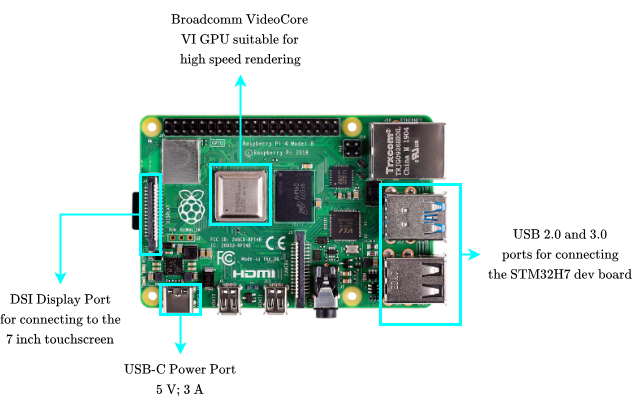
\includegraphics[width=0.64\linewidth]{Figures/Methodology/dps-rpi-4b}
		\caption{Parts of the \acrshort{rpi} 4B that are of particular interest for this project.}
		\label{fig:dps-rpi-4b}
	\end{figure} 

	The \acrshort{rpi} 4B can also connect to both the STM32H723ZG microcontroller or Picoscope 2204A via \acrshort{usb} to integrate the \acrshort{dps} with the \acrshort{das}. Figure \ref{fig:dps-rpi-4b} of the \acrshort{rpi}. A Raspberry Pi \acrshort{os} image is flashed to a \acrshort{sd} card using Raspberry Pi imager, then the Python scripts for running the \acrshort{dps} and \acrshort{guis} operations is loaded and executed on the device. 
	
	Each division in the displayed amplitude vs frequency spectrogram is mapped to the sampled input voltages which are input to the \acrshort{dps}. Given that the vertical output of the HP141T is inverted and scaled in the \acrshort{scs}, the \acrshort{dps} associates the $\SI{0}{\volt}$ to $\SI{3.3}{\volt}$ $\texttt{V}_\texttt{y}$ input with a vertical axis with values up to 80 $\si{\decibel}$. This is in line with the plot shown on the \acrshort{crt} display of the HP141T system which uses $\SI{0.1}{\volt}$ per division scaling to represent the amplitude on 8 divisions of $\SI{10}{\decibel}$ each (in line with UR03). Different stages of the vertical output are illustrated in figure \ref{fig:dps-vertical-scaling} to inform the \acrshort{svsis} and \acrshort{evsis} for converting data to the appropriate scale and performing interpolation to ensure that a continuous spectrum can be displayed. 
	\begin{figure}[ht!]
		\centering
		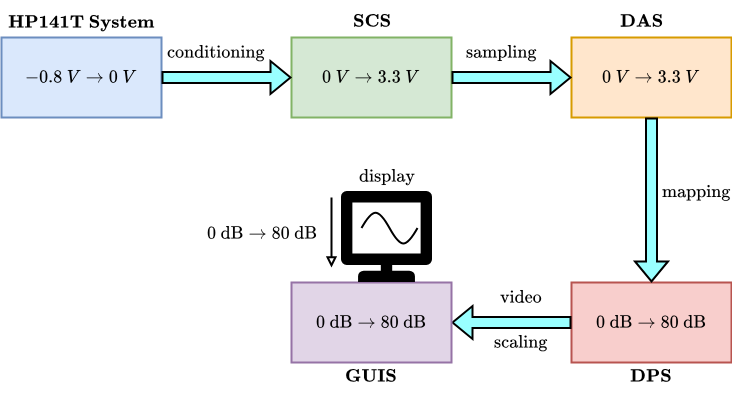
\includegraphics[width=0.58\linewidth]{Figures/Methodology/dps-vertical-scaling}
		\caption{Illustrating the output voltage range associated with each subsystem. The operation performed by the subsystem is shown above the arrow preceding the block containing the output range of that subsystem.}
		\label{fig:dps-vertical-scaling}
	\end{figure} 
	The schematic of the flow of the vertical output at different stages in each subsystem shows that since the \acrshort{scs} inverts the scales the HP141T's auxiliary signal to $\SI{0}{\volt}$ to $\SI{3.3}{\volt}$, the original negative maximum of $-\SI{0.8}{\volt}$ is mapped to $\SI{0}{\volt}$ at the \acrshort{adc} stage. Similarly, the original zero minimum voltage maps to the maximum voltage of the \acrshort{adc}. To prepare the data for display on the amplitude vs frequency plot, the \acrshort{dps} maps the \acrshort{adc}'s $\SI{0}{\volt}$ to $\SI{0}{\decibel}$ and uses a linear mapping to plot the points along the vertical axis. For example, given that $\SI{0}{\volt}$ to $-\SI{0.8}{\volt}$ maps to $\SI{3.3}{\volt}$ to $\SI{0}{\volt}$, the \acrshort{adc} sample $\texttt{V}_\texttt{y}$ can be converted to the 80-$\si{\decibel}$ using
	\begin{align}
		\si{\decibel}	& = 80\times \frac{(\SI{3.3}{\volt} - \texttt{V}_\texttt{y})}{\SI{3.3}{\volt}}
	\end{align} 
	so that each $\SI{0.1}{\volt}$ shift corresponds to $\SI{10}{\decibel}$. 
	
	Preparations for displaying the HP141T Emulator vertical output are performed in a similar manner to the one described above for scaling the vertical output of the HP141T \acrshort{sa} to the required $\SI{80}{\decibel}$ amplitude range.  However, the expected input range is mapped from [$\SI{0}{\volt}$, $\SI{3.0}{\volt}$] to [$\SI{80}{\decibel}$].
	
	The horizontal output is mapped to the frequency axis to represent the scan rate. The original output range of the HP141T system's sawtooth function is [$-\SI{5}{\volt}$, $\SI{5}{\volt}$]. After the signal is conditioned through the operational amplifier-based circuit in \acrshort{scs}, values range between $\SI{0}{\volt}$ and $\SI{3.3}{\volt}$. Time domain characteristics of the scan output do not change during the signal conditioning process - suggested by the simulation results. This implies that the time column in the \texttt{.csv} file is used directly to display the frequency axis on the display with 10 horizontal divisions. The sawtooth rise-time represents the frequency sweep. For 801 points at 7.2 \acrshort{msps}, each division corresponds to $\SI{0.0111}{\milli\second}$. 
	
	The \acrshort{dps} assumes that the HP141T is operating in FULL SCAN mode where the whole tuning section band is displayed. The tuning section, or \acrshort{rf} section, measures frequencies between $\SI{20}{\hertz}$ and $\SI{18}{\giga\hertz}$ with the center frequency is marked on the \acrshort{crt} display. The design is expected to work for the PER DIVISION mode which allows for different scan rates to enable signal analysis. 
	
	The \acrshort{dps} uses default linear interpolation associated with the \texttt{ax.plot} which is considered to be sufficient for this application given the large sampled data set. This is to say that the time between points ($\SI{0.139}{\micro\second}$) is small enough that linear segments should appear smooth in the \acrshort{guis} display. The design explores alternative methods such as Spline interpolation which fits a piecewise polynomial through the data points. Implementation of Spline interpolation is expected to reduce sharp transitions that typically appear with linear interpolation by increasing the resolution to 1000 points so that the curve appears continuous. This type of interpolation is executed using the \texttt{scipy.interpolate} module's \texttt{CubicSpline} function which interpolate vertical output data in both the \acrshort{svsis} and \acrshort{evsis} as shown in the code snippet in listing \ref{lst:dps-spline} in the appendix. 
	
	\subsection{Graphical User Interface Subsystem}
	
	The \acrshort{guis} uses \acrshort{gui} libraries such as \texttt{matplotlib} and \texttt{tkinter} to render the amplitude vs frequency plot on the digitized \acrshort{sa}. The \acrshort{gui} libraries interface with the \acrshort{rpi}'s framebuffer, through which the \acrshort{dps} sends video data for drawing directly to the screen. The final image frame is pushed directly to \texttt{/dev/fb0} to ensure that frequency domain data is rendered in real-time on the display based on the processed outputs of the \acrshort{dps}.
	
	Table \ref{tab:guis-properties} gives a description of the properties of the \acrshort{guis} which replicates the HP141T's \acrshort{crt} graticule. 
	\begin{table}[ht!]
		\centering
		\label{tab:guis-properties}
		\begin{tabular}{|m{5em}|m{15em}|m{10em}|}
			\hline
			\rowcolor{cyan!25} \textbf{Property}	& \textbf{Description}	& \textbf{Associated Values}\\
			\hline
			Vertical Axis	& Mapping of \acrshort{adc} samples to match the scaling on the original HP141T display.	&  $\SI{80}{\decibel}$ scale ($\SI{10}{\decibel}$ per division)\\
			\hline
			Horizontal Axis & Mapping of scan time to the frequency in alignment with the HP141T's sweep display & 10 divisions of the scan outputs progression\\
			\hline
			Grid	& A grid replicating the \acrshort{crt} graticule. & 8x10 grid (8 amplitude divisions, 10 scan time divisions)\\
			\hline
			\acrshort{crt} Appearance & A black background colour with a green trace and grey grid lines to resemble the aesthetic of the \acrshort{crt}. & black = $\#000000$; green = $\#0080000$; grey = $\#808080$\\
			\hline
			Touchscreen	& \acrshort{tft} \acrshort{dsi} capacitive touchscreen display which enables the user to access different modes. & 7 inches with 800x480 resolution\\
			\hline
		\end{tabular}
		\caption{Highlighted properties of the \acrshort{guis}.}
	\end{table}
	
	The \acrshort{guis} employs the \texttt{hp141t} Python module containing functions for enabling the \acrshort{phm}, \acrshort{avm}, and \acrshort{rwm}. The module functions belong in the \acrshort{dps} for processing vertical output data and provides interpolated outputs to the \acrshort{guis}. Code snippets for the functions in the \texttt{hp141t} module are included in listing \ref{lst:guis-phm} in the +appendices section.
		
	The code for the \acrshort{phm} tracks and displays the maximum value seen for each time point and updated per scan when user selects the \texttt{PHM} button. For the \acrshort{avm}, the \acrshort{dps} computes a running average, updated at each scan, and the \acrshort{guis} displays the output to the user when the \texttt{AvM} button is selected on the touchscreen. The \acrshort{guis} also displays the latest value, overwriting previous values during each scan. During system initialization, the \acrshort{guis} sets the default mode to \acrshort{rwm} and initializes the \texttt{peak\_data} and \texttt{raw\_data} data arrays for storing the output associated with each mode. The output of the \acrshort{avm} is weighted by scan count.
	
	Button functions set the modes independently so that the \acrshort{guis} operates in one mode at a time. Each button function calls \texttt{processor.set\_mode} and updates the display to ensure that the user maintains control. Buttons have a simple design with rounded edges, while adhering to Nielsen's design heuristics. 
	
	To fulfil the requirement for system to have tutorials and documentation to help users (SR06), a \texttt{show\_help} function, shown in listing \ref{lst:guis-show-help}, is associated with a \texttt{HELP} button which creates a pop-up window with a tutorial. The tutorial is displayed in a 400x300 pixel window with a black background. The content of the tutorial covers the purpose of the design, available modes, usage instructions and notes on the HP141T system. 
	
	\section{Experimental Test Procedures}
	
	The following section details the methodology and setup used to verify the functionality and performance of the proposed design for the modernized HP141T \acrshort{sa}. Experimental procedures are divided into three main categories, namely, unit tests, integration tests and acceptance tests. Unit tests are designed to validate the correctness of the individual subsystem software and hardware interfaces in isolation. 
	
	Integration tests are designed to evaluate the interactions between subsystems to ensure that the subsystems work as expected with the HP141T system which includes the \acrshort{if} and \acrshort{rf} sections. Acceptance tests assess the system's compliance with the user and system requirements shown in tables \ref{tab:user-requirements} and \ref{tab:sys-requirements}. Included are the test environments, tools and tasks for systematically evaluating the behaviour of each subsystem and the overall system. Tools for supplying power and performing measurements during hardware-based tests included:
	\begin{itemize}
		\item 
		Siglent SDG1010 $\SI{10}{\mega\hertz}$ function generator for producing the modelling the auxiliary outputs of the HP141T, as well as noisy signals for non-ideal cases.
		\item 
		HPE3630A Triple Output DC Power Supply with $\SI{0}{\volt}-\SI{6}{\volt}$, $\SI{2.5}{\ampere}$ outputs, or $\SI{0}{\volt}$ - $\pm\SI{20}{\volt}$, $\SI{0}{\volt}$ - $\SI{0.5}{\ampere}$ outputs.
		\item 
		Picoscope 2204A \acrshort{usb} oscilloscope with two analog channels and maximum input frequency of $\SI{10}{\mega\hertz}$.
		\item 
		Oscilloscope probes with 10x scaling capabilities.
	\end{itemize}
	The Picoscope 2204A was used together with the Picoscope 7 Software to measure analog signals in all experiments. The oscilloscope was connected to a \acrshort{usb} 3.0 port of a Linux-based Dell Inspiron 15 machine and outputs were analyzed using the Picoscope 7 software on the machine. 
	\subsection{Unit Tests for Subsystem Verification}
	\subsubsection{HP141T System Unit Tests}
	Unit tests for the HP141T system were advised by the datasheets of the HP8555A and HP8552B plug-in sections. The following unit test procedures were considered for the HP141T system. In the description of each unit test, it is assumed that the Picoscope is connected via \acrshort{usb} to the computer on which the Picoscope 7 software is executed.
	
	\begin{center}
		\textbf{UTA00}: \textbf{Vertical Output Voltage Range} 
	\end{center}
	Connect an input to the HP8555A with a frequency between $\SI{20}{\mega\hertz}$ to $\SI{18}{\giga\hertz}$. Check that the Picoscope environment is running. Connect the vertical output (Y) of the HP8552B to channel A of the Picoscope 2204A using oscilloscope probes. Set the scaling to 10x on the oscilloscope and the probe connected to channel A. Ensure that the Vertical Channel Options for A are set to \texttt{Auto}, the voltage scaling to $\pm\SI{1}{\volt}$, and that \texttt{Invert} is \texttt{Off}. The measured voltage on channel A should be between $\SI{0}{\volt}$ and $-\SI{0.8}{\volt}$. If there is no input at the HP8555A plug-in, then the voltage should be $\SI{0}{\volt}$. 
	
	\begin{center}
		\textbf{UTA01}: \textbf{Vertical Output Frequency Range}  
	\end{center}
	With the vertical output connected to channel A, and the Picoscope 7 software running, click on \texttt{View} and select spectrum. The spectrum should contain frequency components between $\SI{10}{\hertz}$ and $\SI{300}{\hertz}$.
	
	\begin{center}
		\textbf{UTA02}: \textbf{Horizontal Output Voltage Range} 
	\end{center}
	Connect the horizontal output of the HP141T to channel B of the Picoscope and select the channel in the software. The signal should look like a sawtooth function ranging between $\pm\SI{5}{\volt}$ and a rise time of up to 1 div/$\si{\micro\second}$. 
	
	\begin{center}
		\textbf{UTA03}: \textbf{Pen-Lift Output Voltage Range}
	\end{center}
	Disconnect the probes from HP141T \acrshort{sa}. Remove the probe connected to channel B. Connect the probe associated with channel A to the pen-lift output of the HP141T. The signal displayed in the oscilloscope's software should range between $\SI{0}{\volt}$ and $\SI{14}{\volt}$. 
	
	\subsubsection{HP141T Emulator Unit Tests}
	Unit tests for the HP141T Emulator were developed based on the expected behavior of the analog outputs and the digital processing pipeline. These tests verify the signal characteristics produced by the emulator and ensure that the ADC sampling, signal conditioning, and waveform generation circuits function as designed. It is assumed that a Picoscope 2204A is connected to the system and controlled via the Picoscope 7 software.
	
	\begin{center}
		\textbf{UTB00}: \textbf{Emulated Vertical Output Voltage Range}
	\end{center}
	Run the emulator and ensure a test signal (sinusoidal or modulated RF) is applied to the ADC input. Connect the emulator’s vertical output to channel A of the Picoscope. Ensure the vertical scaling is set to $\pm\SI{5}{\volt}$ and the probe attenuation is 10x. The observed voltage should range between $\SI{0}{\volt}$ and $\SI{3.0}{\volt}$.
	
	\begin{center}
		\textbf{UTB01}: \textbf{Emulated Vertical Output Frequency Range}
	\end{center}
	With the vertical output still connected to channel A, switch to spectrum view in Picoscope 7. The frequency components of the vertical signal should be $\SI{10}{\hertz}$, consistent with the design.
	
	\begin{center}
		\textbf{UTB02}: \textbf{Emulated Horizontal Output Voltage Range}
	\end{center}
	Connect the horizontal output of the emulator to channel B. The signal should appear as a ramp or sawtooth waveform with a voltage swing between $-\SI{4.76}{\volt}$ and $+\SI{4.75}{\volt}$. The period should correspond to the configured scan time base (e.g., 1 ms to 100 s per sweep).
	
	\begin{center}
		\textbf{UTB03}: \textbf{Pen-Lift Output Voltage Range}
	\end{center}
	Connect channel A to the emulator’s pen-lift output. When scanning is active, the pen-lift output should be $\SI{0}{\volt}$. During retrace (i.e., blanking interval), the output should rise to approximately $\SI{14}{\volt}$. Confirm that this toggling corresponds with the sawtooth waveform transitions on the horizontal output.
	
	\begin{center}
		\textbf{UTB04}: \textbf{HP141T Power Supply}
	\end{center}
	Ensure the HP141T Emulator is powered by the designated plug-in AC/DC adapter rated at $\SI{12}{\volt}$, $\SI{1}{\ampere}$ maximum output. With the emulator powered on, use a multimeter or oscilloscope to measure the voltage at the outputs of all power rails generated by internal regulators and inverter circuits. Confirm the following:
	
	\begin{itemize}
		\item \textbf{+3.3V rail}: Output must be within $\SI{3.3}{\volt} \pm \SI{0.1}{\volt}$, used for ADCs and digital logic.
		\item \textbf{-5V rail (if generated)}: Output must be within \SI{-5}{\volt} $\pm$ \SI{0.2}{\volt}, used for op-amps or analog reference circuits.
		\item \textbf{+5V or +12V rail}: Check regulator outputs for subsystems such as op-amps or display drivers.
	\end{itemize}
	
	Use an oscilloscope to check for voltage ripple and noise on each power rail. Verify that ripple does not exceed $\SI{50}{\milli\volt}$ under load. Confirm that startup transients settle within $\SI{10}{\milli\second}$. This test ensures the emulator's power delivery is stable and within tolerance for all connected subsystems.
	
	\subsubsection{\acrlong{scs} Unit Tests}
	The \acrfull{scs} is responsible for scaling, shifting, and inverting the auxiliary analog outputs from the HP141T system so they can be sampled accurately by the \acrshort{adc}s. Unit testing of this subsystem focuses on validating voltage range translation, signal polarity, and waveform integrity. All tests assume that the outputs are probed using a calibrated Picoscope 2204A with appropriate probe attenuation (10x) and configured channel settings. 
	
	\begin{center}
		\textbf{UTC01}: \textbf{Vertical Output Inversion and Scaling}
	\end{center}
	Power the \acrshort{scs} \acrshort{pcb} by a $\SI{9}{\volt}$ DC supply - the green LED on the board should turn on to indicate that the circuit is operational.
	
	\begin{center}
		\textbf{UTC01}: \textbf{Vertical Output Inversion and Scaling}
	\end{center}
	Apply a known signal to the vertical output of the HP141T (e.g., sinusoidal waveform with a peak-to-peak voltage between up to $\SI{0.8}{\volt}$). Connect this output to the \acrshort{scs} input and probe the output with channel A of the Picoscope. Verify that the signal is inverted and scaled such that $-\SI{0.8}{\volt}$ corresponds to $\SI{0}{\volt}$ and $\SI{0}{\volt}$ corresponds to approximately $\SI{3.3}{\volt}$. Use the measurement cursor to confirm linear scaling.
	
	\begin{center}
		\textbf{UTC02}: \textbf{Horizontal Output Linear Scaling}
	\end{center}
	Input a test sawtooth waveform into the horizontal output path of the HP141T. Connect the SCS output to channel B and compare the measured waveform to the known input. Confirm that the SCS output exhibits a full-scale ramp from $-\SI{5}{\volt}$ to $+\SI{5}{\volt}$ mapped linearly to the $\SI{0}{\volt}$ to $\SI{3.3}{\volt}$ range, preserving waveform shape and ramp symmetry.
	
	\begin{center}
		\textbf{UTC03}: \textbf{Pen-Lift Output Logic Level Shifting}
	\end{center}
	Apply a manual scan trigger to the HP141T system to induce a pen-lift event. Connect the \acrshort{scs} output for the pen-lift signal to channel A. The output should transition from approximately $\SI{0}{\volt}$ (during scan) to a logic high voltage of $\SI{3.3}{\volt}$ when blanking is active. Verify that the logic levels remain within acceptable digital input thresholds for the \acrshort{adc} and digital processing stages.
	
	\begin{center}
		\textbf{UTC04}: \textbf{Signal Integrity and Noise Margin}
	\end{center}
	With the \acrshort{scs} outputs connected to the Picoscope, enable high-resolution mode and apply bandwidth filtering to assess signal noise and distortion. Verify that output signals maintain consistent voltage levels without oscillation, excessive ripple, or overshoot. Measure peak-to-peak noise and confirm that the noise margin is within acceptable limits (e.g., less than $\SI{20}{\milli\volt}$ for a steady signal).
	
	\begin{center}
		\textbf{UTC05}: \textbf{Response to Overvoltage and Fault Conditions}
	\end{center}
	Apply an out-of-range voltage (e.g., $\pm\SI{10}{\volt}$) to each input line of the \acrshort{scs} one at a time. Monitor the output with the Picoscope. Confirm that the subsystem clamps or safely rejects the signal without passing excessive voltage to the \acrshort{adc} inputs.
	
	\subsubsection{\acrlong{das} Unit Tests}
	The \acrshort{das} is responsible for sampling the conditioned analog signals from the HP141T Emulator, digitizing them using high-speed ADCs, and storing the values for further processing in the \acrshort{dps}. The following unit tests verify correct sampling behavior, signal integrity, timing, and storage functionality.
	
	\begin{center}
		\textbf{UTD00}: \textbf{\acrshort{adc} Voltage Input Range Test}
	\end{center}
	Apply known \acrshort{dc} voltages within the expected input range (e.g., 0V, 1.65V, and 3.3V) to each \acrshort{adc} input channel ($\texttt{V}_\texttt{x}$, $\texttt{V}_\texttt{y}$, $\texttt{V}_\texttt{z}$). Sample the inputs using the \acrshort{das} and export the resulting values to a \texttt{.csv} file. Verify that the digital values correspond to the expected 16-bit quantization of the input voltages, using:
	\[
	V_{\text{in}} = \frac{\text{\acrshort{adc} Output}}{65535} \times \SI{3.3}{\volt}
	\]
	
	\begin{center}
		\textbf{UTD01}: \textbf{Sampling Rate Verification}
	\end{center}
	Configure the DAS to run at the target sampling rate (e.g., 7.2 \acrshort{msps}). Using a signal generator, apply a known frequency signal (e.g., $\SI{1}{\mega\hertz}$ sine wave) to an \acrshort{adc} channel. Use the time stamps in the \texttt{.csv} output to compute the effective sampling interval and verify that the measured sampling rate is within ±5\% of the configured value.
	
	\begin{center}
		\textbf{UTD02}: \textbf{Multi-Channel Synchronization Test}
	\end{center}
	Apply identical signals to all three \acrshort{adc} input channels and run the sampling routine. Compare the sampled waveforms from the \texttt{.csv} output to confirm that the channels are sampled in sync or with known interleaving, based on the expected \acrshort{adc} configuration. Check for time alignment by comparing signal edges or zero crossings.
	
	\begin{center}
		\textbf{UTD03}: \textbf{Signal Integrity}
	\end{center}
	Apply a low-noise sine wave signal to an \acrshort{adc} input and record the sampled data. Analyze the resulting waveform for quantization noise and distortion using FFT. Verify that the signal-to-noise ratio (\acrshort{snr}) and effective number of bits (\acrshort{enob}) match the \acrshort{adc}’s datasheet specification within tolerance.
	
	\begin{center}
		\textbf{UTD04}: \textbf{File Writing}
	\end{center}
	Run the \texttt{spectrogram\_to\_csv()} function after a complete data capture session. Open the generated \texttt{.csv} files and verify the format:
	\begin{itemize}
		\item Header row includes <Time ($\si{\milli\second}$), $\texttt{V}_\texttt{x} (\si{\volt})$, $\texttt{V}_\texttt{y} (\si{\volt})$, $\texttt{V}_\texttt{z} (\si{\volt})$>
		\item Each row is correctly formatted with numerical values
		\item All expected sample points are recorded (e.g., 801 samples per file)
	\end{itemize}
	
	\begin{center}
		\textbf{UTD05}: \textbf{Pause/Resume Functionality}
	\end{center}
	Use the touch interface to trigger a pause during data capture. Confirm that data acquisition halts immediately and resumes only when the pause flag is cleared. Ensure that partial files are properly closed and new files are opened after resuming.
	
	\subsubsection{\acrlong{dps} Unit Tests}
	
	The \acrshort{dps} is responsible for interpreting sampled \acrshort{adc} data, applying transformations such as scaling and interpolation, and preparing the data for display in various user-selectable modes. The following unit tests verify the correctness of mathematical processing, mode switching, and data integrity.
	
	\begin{center}
		\textbf{UTE00}: \textbf{Spectrogram Data Scaling Verification}
	\end{center}
	Load a \texttt{.csv} file with known voltage values into the \acrshort{dps} and process it using the standard vertical scaling equation:
	\[
	\text{dB} = 80 \times \frac{(3.3 - V_y)}{3.3}
	\]
	Verify that the resulting amplitude values match expected decibel levels (e.g., a 0V input maps to 80 dB and 3.3V to 0 dB).
	
	\begin{center}
		\textbf{UTE01}: \textbf{Peak Hold Mode Accuracy}
	\end{center}
	Feed multiple spectrograms with varying amplitudes into the \acrshort{dps}. Confirm that the \texttt{max()} function correctly retains the highest amplitude observed for each frequency bin across scans.
	
	\begin{center}
		\textbf{UTE02}: \textbf{Average Mode Calculation Accuracy}
	\end{center}
	Run the \texttt{average\_spectrogram()} function over multiple scans. Confirm that each bin’s output is the correct arithmetic mean of its values from all prior scans.
	
	\begin{center}
		\textbf{UTE03}: \textbf{Interpolation Output Continuity}
	\end{center}
	Input coarse or gapped spectrogram data into the \acrshort{dps}. Verify that the interpolation algorithm produces a continuous, visually smooth spectrum with no missing or duplicated points.
	
	\begin{center}
		\textbf{UTE04}: \textbf{Spectrogram Data Pipeline Integrity}
	\end{center}
	Verify that all expected data points from the \texttt{.csv} input are preserved throughout the DPS processing pipeline and correctly passed to the GUI plotting module.
		
	\subsubsection{\acrshort{guis} Unit Tests}
	The \acrshort{guis} runs on the Raspberry Pi 4B and is responsible for rendering the processed spectrogram data, managing user inputs via touchscreen, and switching between display modes. The following unit tests ensure correct visualization, responsiveness, and display scaling.
	
	\begin{center}
		\textbf{UTE05}: \textbf{Display Scaling Verification}
	\end{center}
	Load a set of scaled decibel values from the \acrshort{dps} into the \acrshort{gui} rendering module. Confirm that each 10 dB increment correctly maps to one vertical division on the \acrshort{gui} plot.
	
	\begin{center}
		\textbf{UTE06}: \textbf{Touchscreen Mode Switching}
	\end{center}
	Verify that all \acrshort{gui} buttons (e.g., Average, Peak Hold, Raw) correctly update the active display mode and the interface reflects the change without delay.
	
	\begin{center}
		\textbf{UTE07}: \textbf{Real-Time Plot Update Rate}
	\end{center}
	Run the \acrshort{gui} using a constant stream of spectrogram data and measure the update rate. Verify that the display refreshes in near real-time (e.g., every 50–100 ms) with minimal lag.
	
	\begin{center}
		\textbf{UTE08}: \textbf{Graph Rendering Accuracy}
	\end{center}
	Input a known waveform or fixed dataset into the \acrshort{guis}. Visually verify that the plot matches expected amplitude vs frequency behavior. Compare screen coordinates to underlying data values to confirm accuracy.
	
	\begin{center}
		\textbf{UTE09}: \textbf{Pause and Resume Functionality}
	\end{center}
	Press the pause/resume button on the \acrshort{gui} while data is being processed. Confirm that data acquisition halts immediately, and resumes without loss of continuity or data corruption when resumed.
	
	\subsection{Integration Tests for Overall Digitized HP141T System Verification}
	
	Integration tests were performed to verify that the individual subsystems—namely the \acrshort{scs}, \acrshort{das}, \acrshort{dps}, and \acrshort{guis}—function correctly when combined. These tests ensured that signals flowed correctly between stages and that each interface (analog, digital, and software) operated as expected. For example, outputs from the \acrshort{scs} were validated at the \acrshort{das} input, and the data exported from the \acrshort{das} was processed and visualized through the \acrshort{dps} and \acrshort{guis}. The integration tests focused on detecting mismatches in voltage ranges, data formats, timing synchronization, and communication between hardware and software components.
	
	\subsection{Acceptance Tests} 
	
	Acceptance testing evaluated the system against the functional requirements defined early in the project, such as accurate signal acquisition, support for multiple display modes, and successful user interaction through the \acrshort{gui}. These tests confirmed the system's readiness for real-world use and assessed overall usability, responsiveness, and fidelity of the emulator in replicating the HP141T’s behavior. Each requirement was validated by comparing the digitized system's output to reference measurements from the original HP141T system or expected theoretical behavior, ensuring that the design met its intended performance and user expectations.
	% ----------------------------------------------------
	\ifstandalone
	\bibliography{../Bibliography/References.bib}
	\printnoidxglossary[type=\acronymtype,nonumberlist]
	\fi
\end{document}
% ----------------------------------------------------